\documentclass{ruthesis}
\usepackage{graphicx}          % Include this line if your
                               % document contains figures,
%\usepackage[dvips]{epsfig}    % or this line, depending on which
                               % you prefer.

\usepackage{listings}
\lstset{breaklines=true}
\lstset{numbers=left, numberstyle=\scriptsize\ttfamily, numbersep=10pt, captionpos=b} 
\lstset{basicstyle=\small\ttfamily}
\lstset{framesep=4pt}
\usepackage{amsfonts,amssymb,amsbsy}
\usepackage{latexsym}
\usepackage{amsmath}
\usepackage{color}
\usepackage{graphics} % for pdf, bitmapped graphics files
\usepackage{epsfig} % for postscript graphics files
\usepackage{epstopdf}
\usepackage{caption}
\usepackage{subcaption}
\usepackage{longtable}
\usepackage{multirow}
\usepackage{afterpage}
\usepackage{array,booktabs,enumitem}% http://ctan.org/pkg/
\newcolumntype{P}[1]{>{\endgraf\vspace*{-\baselineskip}}p{#1}}
%\usepackage{graphicx,subfigure}
%\usepackage{rotating}
%\usepackage{theorem}
%%\usepackage{isomath}
%\usepackage{mathrsfs}
%\usepackage{enumerate}

\usepackage{placeins}
\usepackage{rotating}
\usepackage{titlesec}
\usepackage{geometry}
 \geometry{
 a4paper,
 total={210mm,297mm}, left=20mm, right=20mm, top=20mm, bottom=20mm,}
 
\def\etal{\mbox{et al.}}
\DeclareMathOperator*{\sign}{sign}
\DeclareMathOperator*{\diag}{diag}
\DeclareMathOperator*{\proj}{proj}
\DeclareMathOperator*{\argmin}{argmin}
\DeclareMathOperator*{\rank}{rank}
\newcommand{\norm}[1]{{{\lVert #1 \rVert}}}
\newcommand{\clN}{{\cal N}}
\newcommand{\clM}{{\cal M}}
%\newcommand{\diag}{{\sf diag}}
%\newcommand{\sgn}{{\sf sgn}}
\newtheorem{proposition}{Proposition}
\newtheorem{theorem}{Theorem}
\newtheorem{lemma}{Lemma}
\newtheorem{corollary}{Corollary}
\newtheorem{remark}{Remark}
\newtheorem{definition}{Definition}
\newtheorem{assumption}{Assumption}

\setlength{\parskip}{0.2cm} 
\setlength{\topmargin}{-0.4cm}
\setlength{\oddsidemargin}{1cm} 
\setlength\evensidemargin{1cm}
\setlength{\textwidth}{15cm} 
\setlength{\textheight}{23.5cm}
\titlespacing\section{-4pt}{12pt plus 4pt minus 2pt}{0pt plus 2pt minus 2pt}
\titlespacing\subsection{0pt}{12pt plus 4pt minus 2pt}{0pt plus 2pt minus 2pt}
\titlespacing\subsubsection{0pt}{12pt plus 4pt minus 2pt}{0pt plus 2pt minus 2pt}
\titleformat{\subsubsection}
  {\bfseries\itshape\normalsize}{\thesubsubsection}{1em}{}

\usepackage[version=4]{mhchem}
\usepackage{chemist}

\begin{document}
\tableofcontents

\pagenumbering{arabic}
\linespacing{1.7}

\setcounter{chapter}{3}
\chapter{A data assimilating state-space model for algal growth under controlled conditions within a photo-bioreactor}\label{ch:micro_chapter}

\section{Introduction}\label{sec:micro_intro} 

The key goal of biofuels production is the optimisation of biomass productivity in large-scale microalgal culturing systems such as open ponds or closed photo-bioreactors. The primary goal is to maximise the production of raw biomass.   

Microalgae has long been viewed as a potential platform for bioengineering.  During the 1970's and 2000's much of the research focussed on biofuel production, while recently the potential for pharmaceuticals and other high-value chemicals has been explored.  Whether the desired product is a primary metabolite (eg lipids in biofuel production) or secondary metabolite (eg astaxanthin as high-value dye) it is important to be able to measure processes such as photosynthesis and respiration that take place in the cells.   




At the broadest scale the growth of microalgae can be expressed as the following chemical reaction in which \ce{C} is taken from the atmosphere as \ce{CO_2}, along with aqueous nutrients \ce{N} and \ce{P}, to produce biomass

\begin{align*}
\ce{
 106 CO_2(g)  + 122 H_2O  + 16  NO_3^-(aq)  + PO_4^{3-}(aq)  + 19 H^+}\nonumber\\
 \ce{
  \reactrarrow{0pt}{2.5cm}{$\left[10^3-10^4\right]\gamma$}{} C_{106} H_{263} O_{110} N_{16} P_1 + 138 O_2 (g)}\\ 
\end{align*}%\label{eq:chem_simple)

This equation captures a number of features of interest.  The total biomass is determined by the concentrations of \ce{N} and \ce{P}. A typical growth media for microalgae is Guillard's Marine Enriched Seawater (F/2), which has Nitrogen concentration of 880$\mskip3mu$$\mu$M, Phosphorus concentration of 36$\mskip3mu$$\mu$M, and total alkalinity of 2300$\mskip3mu$$\mu$M.
 
%\begin{table}[h] 
%	\begin{tabular}{ |c|r|} 
%		\textbf{species} & \textbf{conc} / $\mu$M \\ 
%		\hline 
%		N  &   880 \\ 
%		P   &   36  \\ 
%		TA & 2300 		
%	\end{tabular} 
%\end{table} 

\begin{itemize}
\item{\textbf{Biomass}:} Taking the limiting nutrient to be Nitrogen, the maximum biomass of algae is 200$\mskip3mu$mg L$^{-1}$, of which about 70$\mskip3mu$mg L$^{-1}$ is Carbon.  This is equivalent  0.12$\mskip3mu$L of pure \ce{CO_2} At Standard Temperature and Pressure, which around to 325$\mskip3mu$L of air for each litre of media.

\item{\textbf{Change in alkalinity}:} Alkalinity is central concept in seawater chemistry that allows one to calculate how much Carbon can be dissolved in solution, and what form it takes (Dissolved Inorganic Carbon exists as \ce{CO_2}, \ce{HCO_3^-} and \ce{CO_3^{2-}}).  Alkalinity measures the charge imbalance between strongly and weakly dissociating ions in solution.  As the charged nutrients are removed from the solution during growth the alkalinity increases and more Carbon is able to be dissolved in the media.  For PBR F/2 media the initial TA is 2300.  

\end{itemize} 

 

Look at the fluxes into and out the system, like respiromtery. 


Carbon and light availability are two of the most common limiting factors of biomass productivity \cite{posten2009design}.


The key goals of this chapter are to,
\begin{itemize} 
	\item{} Develop more understanding of processes in high temporal resolution which are non-destructive.   	
	\item{} 'Fuse' high resolution measurements with more direct measurements.  	
	\item{} Incorporate prior information and constraints on parameters. 
\end{itemize} 



%[BM for ref: At 2 hour intervals, a solenoid valve (SMC Pneumatics Pty. Ltd.) was used to stop aeration for 10 minutes. The linear increase in DO caused by these artefacts were used to calculate net photosynthesis. (reference Tamburic 2015)]





\section{Methods}

\subsection{Data Model: Photo-bioreactor setup, experimental design and data collection methods}\label{sec:micro_data_collection}

All data collection methods for this chapter were part of a series of experiments examining microalgal responses to photobiorector treatments (Peter Wood 2019 UTS PhD).

Microalgal culture \emph{Nannochloropsis oceanica} (Droop) Green (strain CS-179) obtained from the Australian National Algae Culture Collection was cultured in 200$\mskip3mu$mL conical flasks; maintained in an incubator (Labec Pty Ltd) at 20$^{\circ}$C, under an irradiance of
50$\mskip3mu$$\mu$mol$\mskip3mu$m$^{-2}$$\mskip3mu$s$^{-1}$ of cool-white fluorescent light at a 12 hour light/12 hour dark cycle. Stock cultures were grown in F/2 saltwater medium \cite{guillard1962studies} and diluted 5 days prior to the start of experiments to ensure that \emph{N. oceanica} was in the exponential growth phase and not nutrient deprived. F/2 was sparged prior to stock culture dilutions to maximise carbon and oxygen content.  

\emph{N. oceanica} was cultured in four, 500$\mskip3mu$mL environmental photo-bioreactors (ePBRs, Phenometrics Inc) with a 10\% v/v inoculation of stock culture. Top-side illumination over a path length of 25$\mskip3mu$cm was provided by a cool-white light LED, whilst temperature was maintained at 27$^{\circ}$C using a Peltier heater-cooler connected to a water jacket. In-built thermocouples, calibrated against external temperature sensors attached to the Firesting module (TeX4; PyroScience GmbH), measured every 5 minutes were used to control the Peltier heater-cooler jacket through a feedback loop to an accuracy of $\pm$ 0.2$^{\circ}$C. pH was also measured in 5 min intervals by in-built pH electrodes (Van London Inc); controlled by periodic CO2 (5\%) injections using valves in the ePBRs. pH was 3-point calibrated using pH buffer solutions at pH 4.00 $\pm$ 0.02, pH 7.00 $\pm$ 0.02 and pH 10.00 $\pm$ 0.02. PBR mixing was controlled by magnetic stirring bars at 110 rpm. All four ePBRs were aerated with filtered/humidified air through a 1.2$\mskip3mu$mm needle valve (Terumo Co). 


A period of 2 days was allowed for \emph{N. occulata} to acclimate to the ePBRs at an irradiance of 500$\mskip3mu$$\mu$mol$\mskip3mu$m$^{-2}$$\mskip3mu$s$^{-1}$ and a temperature of 27$^{\circ}$C. Following this acclimation period, the ePBR was set to the experimental condition of 2,000$\mskip3mu$$\mu$mol$\mskip3mu$photons$\mskip3mu$m$^{-2}$$\mskip3mu$s$^{-1}$ for another 2 days and a 12 hour light/12 hour dark cycle with a temperature of 27$^{\circ}$C. 
ePBRs were maintained at an optical density (OD) of 0.4 using manual dilutions, creating a semi-batch culturing system. Dilutions occurred once per day (one hour before the light cycle), using aerated F/2 media. The experiment was conducted over a period of 4 days, samples were extracted post and prior dilution, as well as half way through the light cycle. %2$\mskip3mu$mL samples were extracted to measure: OD$_{750}$, cell density, nitrogen concentration and phosphorous concentration. 50$\mskip3mu$mL was extracted to examine alkalinity, dry weight, carbon percentage and nitrogen percentage. 
50$\mskip3mu$mL was extracted to examine total alkalinity and dissolved inorganic carbon. 
%Both pH and DO were measured every 5 mins and 1 min respectively; to generate dynamic daily profiles. 
Dissolved oxygen (DO) was measured using a 3$\mskip3mu$mm robust optical probe (OXROB10-OI; PyroScience GmbH) attached to a FireStingO2 logger (PyroScience GmbH). DO measurements were taken every 60 seconds and temperature-corrected using a temperature extension module (TeX4; PyroScience GmbH). DO was two-point calibrated using air-saturated seawater (100\% saturation) and sodium sulfate-saturated water (0\% saturation). At 2 hour intervals, a solenoid valve (SMC Pneumatics Pty. Ltd.) was used to stop aeration for 10 minutes to allow for observations of net photosynthesis. 

Alkalinity and DIC was measured twice a day closely following the Standard Operating Procedures (SOP) outline in \cite{dickson2007guide}.  Approximately 30$\mskip3mu$mL of \emph{N. oceanica} media was titrated against 0.1$\mskip3mu$M hydrochloric acid on an auto-titrator (800 Dosino; Metrohm AG) [SOP3b Open-cell tritration]. 
The Total Alkalinity and DIC were calculated from the output of the auto-titrator (volume of HCl delivered, pH) by calculating the the pH as a function of the volume of the acid delivered (see SOP3a Annexe 1).
 


\subsection{Data model: Data treatment, distributions and measurement error}\label{sec:micro_data_model}

Gas valve, temperature, light (normalised to 0/1) and dilution rates were used to force the model.
Dissolved oxygen, pH, dissolved inorganic carbon and total alkalinity observations for 4 days post acclimation were assimilated. 
While pH observations were calibrated and corrected, it was visible that $O_2$ observations were not completely calibrated and experienced some sensor drift during the experiment. %An offset term ($offset_{O_2}$) was added to the $O_2$ ode to account for this. The offset was assigned a normally distributed prior distribution with mean 0 and standard deviation 2. [BM:check the offset is still there and you did it this way otherwise change/remove.]

The data model assigned log normally distributed observation errors for each instrument;
$O_{2_{obs}}$ $\sim$ Log$\mathcal{N}$(log($O_2$), $\sigma_{O_2}$), $pH_{obs}$ $\sim$ Log$\mathcal{N}$(log($pH$),  $\sigma_{pH}$), $DIC_{obs}$ $\sim$ Log$\mathcal{N}$(log($DIC$), $\sigma_{DIC}$), $TA_{obs}$ $\sim$ Log$\mathcal{N}$(log($TA$), $\sigma_{DIC}$), where the standard deviations ($\sigma_{O_2}$, $\sigma_{pH}$, $\sigma_{DIC}$) were unknown parameters to be estimated as part of the assimilating model. Dissolved inorganic carbon and total alkalinity measurements were obtained from the same instrument thus the error is shared between these states. %Initial observation error priors started at $\sigma_{O_2}$ $\sim$ Log$\mathcal{N}$(log(0.1), 0.5) and then were adjusted during the PMMH tuning phase. 

\begin{figure}
	\centerline{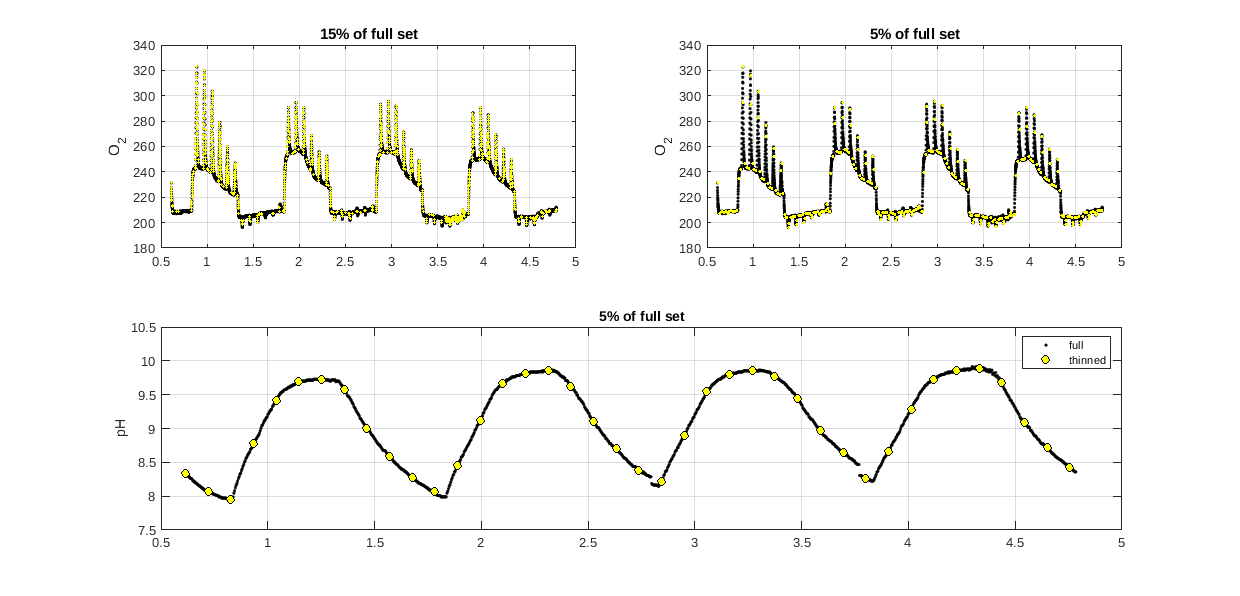
\includegraphics[width=1.25\textwidth]{images_microalgae/plots/thinned_obs_micro}}
	\caption[.]{Full $O_2$ and $pH$ datasets with thinned $O_2$ and $pH$ observations.}
	\label{fig:thinned_obs_micro}
\end{figure}
Due to different instruments used in data collection, $O_2$ observations were collected most frequently (6008 data-points), followed by $pH$ observations (1179 data-points), with $DIC$ and $TA$ collected intermittently (11 data-points). Initial posterior runs with these observation densities resulted in the MCMC chain unable to mix properly due to the high density of observations. In an attempt to improve MCMC mixing, the denser observation sets were thinned/sampled down. The $pH$ observations were thinned to approximately 5\% of the full $pH$ dataset by taking every 30th observation. The $O_2$ observations were thinned to approximately 15\% of the original $O_2$ dataset by only taking those consecutive observations that had at least 1$\mskip3mu$$\mu$M L$^{-1}$ difference (Figure \ref{fig:thinned_obs_micro}).


\FloatBarrier
\subsection{Process model: Carbon chemistry}
%[ Chris : Carbon in seawater summary ]
%main equations and rate constants
%role of TA
%This consists of 4(?) equations with (4?) unknowns

When carbon dioxide dissolves in water it undergoes a series of reactions which results in three species that exist in equilibrium, \ce{CO_2}, \ce{HCO_3^-} and \ce{CO_{3}^{-2}}, accompanied  the release of hydrogen ions.   
CO2SYS is a program developed for CO$_2$ system calculations (CO2SYS) that calculates and returns a detailed state of the carbonate system of oceanographic water samples in seawater and freshwater \cite{lewis1998program}. 
This chemical system as been the focus of extensive research as it central role in understanding the effect of anthropogenic carbon emissions and is generally referred to as ``Ocean Acidification''.   
The dependence of these equilibrium constants on temperature and salinity has been experimentally determined and functional forms have been fitted.   
This has been integrated into  CO2SYS, a program developed for CO$_2$ system calculations that calculates and returns a detailed state of the carbonate system of oceanographic water samples in seawater and freshwater \cite{lewis1998program}.research. 

A thorough explanation of CO2SYS, and seawater carbon chemistry in general, can be found in  Zeebe and Wolf-gladrow \cite{zeebe2001co2}.  A concise summary of the equations can be found in SOP 3a, Annexe 1 of \cite{dickson2007guide}. 

\begin{figure}[h] 
	\centerline{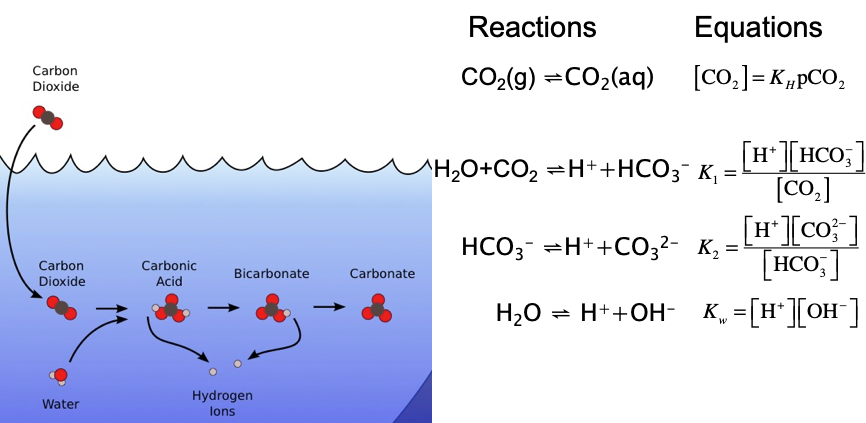
\includegraphics[width=1.0\textwidth]{images_microalgae/CO2sys}} 
	\caption[.]{CO2sys} 
	\label{fig:CO2sys} 
\end{figure} 

It is recognised as the defacto standard for carbon system calculations and is widely used in oceanographic and marine biology.  
Given two of the four measurable carbonate system parameters (total alkalinity, total inorganic CO$_2$, pH, and either fugacity fCO$_2$ or partial pressure of CO$_2$) the other two parameters can be calculated for a set of input conditions (temperature and pressure).  In the model the state variables TA and DIC are given and the pH and pCO$_2$ are calculated.  


Ideally CO2SYS \cite{lewis1998program} would have been used to calculate the carbon chemistry of the photo-bioreactor. 
However,  it is not possible to directly implement CO2sys in LibBi due the constraints imposed by the GP-GPU computing model.  CO2SYS iteratively solves the set of chemical equilibrium equations which requires a for / while loop and if constructs which are not available in LibBI.  
A number of approaches were explored to circumvent this restriction: 
\begin{enumerate} 
	\item{} Creating functional approximation of the solutions from CO2sys 
	\item{} Recasting the steady state equilibrium as a set of coupled ODE's  
	\item{} Manually `unrolling' the while loop as fixed number of iterations.   
\end{enumerate} 

In addition to being tedious, it was not possible to achieve the accuracy needed via functional approximation.   
In particular, ensuring that the invariants of the system (such as non-negativity and that the sum of the carbon species equals the dissolved inorganic carbon) is not trivial.  
The set of ODE's the describe the chemical reactions are notoriously stiff \cite{zeebe1999time} which resulted in a prohibitively small step size.  Coding a fixed number of iterations also presented issues as if the number of iterations is too low the solution is inaccurate while too many iterations is inefficient and may be limited by memory available to the process on the GPU.  

CO2SYS was successfully incorporated into LiBbi  by a combination of the first and third approaches.  The functional approximation from step 1 was used to precondition the solution and 3 iterations were explicitly coded.  (Eq. \ref{newton_raph_iterations1} - \ref{newton_raph_iterations_end}) of the Newton-Raphson method for finding approximations to roots of real valued functions. The Newton-Raphson method is an iterative process 
$ x_{n+1} = x_n - \frac{f(x_n)}{f'(x_n)} $
considering a function $f(x_n)$, its derivative $f'(x_n)$ and an initial starting value $x_0$. The approximate root $x_{n+1}$ converges to the exact solution very quickly if a close initial starting value is picked. To ensure the quick convergence of the Newton-Raphson method, an approximating equation for $pH_0$ (Eq. \ref{pH_approx_eq}) was obtained by fitting a stepwise regression with interactions to a range of simulated CO2SYS input parameters (temperature: 20-30, salinity: 30-40, $DIC$: 200-2500, and alkalinity: 1500-3000). A range of initial conditions and parameter values were tested, and each converged with RMSE $<$ 0.01 across $pH$, $HCO_3^-$, $CO_2$, and $CO_3$, $DIC$, $O_2$, $TA$ by the 3rd iteration (Figure \ref{fig:iterative_carbon_and_states} and Table \ref{table:rmse_iterative}).





%CO2SYS is a program developed for CO$_2$ system calculations (CO2SYS) that calculates and returns a detailed state of the carbonate system of oceanographic water samples in seawater and freshwater \cite{lewis1998program}.
%A thorough explanation of CO2SYS, and seawater carbon chemistry in general, can be found in  Zeebe and Wolf-gladrow \cite{zeebe2001co2}.  A concise summary of the equations can be found in SOP 3a, Annexe 1 of \cite{dickson2007guide}.

%Using two of the four measurable carbonate system parameters (total alkalinity, total inorganic CO$_2$, pH, and either fugacity fCO$_2$ or partial pressure of CO$_2$) to calculate the other two parameters at a set of input conditions (temperature and pressure).  In the model the state variables TA and DIC are given and the pH and pCO$_2$ are calculated. 

%To incorporate CO2SYS into LiBbi for solving carbon chemistry on the timescale of the microalgae model, we explicitly defined 3 iterations (Eq. \ref{newton_raph_iterations1} - \ref{newton_raph_iterations_end}) of the Newton-Raphson method for finding approximations to roots of real valued functions. The Newton-Raphson method is an iterative process 

%HCO$_3^-$, CO$_2$, and CO$_3$ were calculated from the 3rd iteration of pH.


\subsubsection{CO2SYS constants and iterative solution for pH, HCO$_3^-$, CO$_2$, and CO$_3$}

Total Sulfur:
\begin{align*}
TS     	&= \frac{0.14}{96.062} * \frac{S}{1.8065} \nonumber \\
IS     	&= 19.924 \frac{S}{(1000 - 1.005 S)} \nonumber \\
KS_{int} 	&= -\frac{4276.1}{T_K} + 141.328 - 23.093 log(T_K) + (-\frac{13856.0}{T_K} + 324.57 \nonumber\\ 			 
& - 47.986 log(T_K)) \sqrt{IS} + ( \frac{35474}{T_K} - 771.54  + 114.723 log(T_K)) IS \nonumber \\
& - \frac{2698}{T_K} IS^{1.5} + \frac{1776}{T_K} IS^2 \nonumber \\
KS     	&=  (1 - 0.001005 S)e^{(KS_{int})} \nonumber 
\end{align*}

Fluorine:
\begin{align*}
TF       	&= \frac{\frac{0.000067 S}{18.9984}}{1.80655} \nonumber \\
KF       	&= e^{(-(-\frac{874.0}{T_K} - 0.111 \sqrt{S} + 9.68))} \nonumber \\
SWS_{2_T}  	&= \frac{(1 + \frac{TS}{KS})}{(1 + \frac{TS}{KS} + \frac{TF}{KF})} \nonumber \\
Free_{2_T} 	&= 1 + \frac{TS}{KS} \nonumber 
\end{align*}

H2O dissoc:
\begin{align*}
KW 		&= e^{(148.9802 - \frac{13847.26}{T_K}  - 23.6521 log(T_K) 
+ (\frac{118.67}{T_K} - 5.977 + 1.0495 log(T_K)) \sqrt{S} - 0.01615 S)} \nonumber 
\end{align*}

Boron:
\begin{align*}
KB 		&= exp(\frac{(-8966.90 - 2890.53 \sqrt{S} - 77.942 S + 1.728 S \sqrt{S} - 0.0996 S^2)}{T_K} \\
&+ 148.0248 + 137.1942 \sqrt{S} + 1.62142 S \\
&- (24.4344 + 25.085 \sqrt{S} + 0.2474 S) log(T_K) + 0.053105 T_K \sqrt{S}) \nonumber \\
TB 		&= 0.0004326 \frac{S}{35} \nonumber 
\end{align*}

Choice of carbonate dissociation constants $K_1$ and $K_2$ were Mehrbach \cite{mehrbach1973measurement} (refit by Dickson and Millero \cite{dickson1987comparison}) with 1.23$K_1$ and 0.53$K_2$ measured experiment specific adjustments:
\begin{align}
K_1 		&= 10^{(-(\frac{3633.86}{T_K} - 61.2172 + 9.6777 log(T_K) - 0.011555 S + 0.0001152 S^2))}*1.23 \\
K_2 		&= 10^{(-(\frac{471.8}{T_K} + 25.9290 - 3.16967 log(T_K) - 0.01781 S + 0.0001122 S^2))}*0.53 	
\end{align}
%[Choice of H2CO3 and HCO3- dissociation constants $K_1$ and $K_2$ was Mehrbach (refit BY DICKSON AND MILLERO) [BM: After the iterative approach is finalised, the $K_1$ and $K_2$ constants are adjusted based on measurements taken during the experiment, $K_1$*1.23 and $K_2$*0.53 measured during experiment] temperature: 2-35,  salinity: 20-40, Seawater scale, Artificial seawater.]


Approximating equation for the starting value of $pH$: 
\begin{align}
pH_{0} 	&= 12.26 -0.0030605 DIC -0.043752 T -0.013625 S+ 0.00011315 TA \nonumber \\
&+ 1.3463e-5 DIC*T + 5.2215e-7 DIC*TA  \label{pH_approx_eq}	
\end{align}

Newton-Raphson iterations: 
\begin{align}
h_{n} 			&=  10^{-pH_{n}}\label{newton_raph_iterations1}	 \\
h_{n_{free}}	&=  \frac{h_n}{Free_{2_T}}	 \\
f_n				&= (  DIC*1e-6*\frac{K_1 h_n + 2 K_1 K_2}{h_n^2 + K_1 h_n + K_1 K_2}  \nonumber \\
&  - h_{n_{free}} + \frac{KW}{h_n} - TA*1e-6 + \frac{TB}{1+\frac{h_n}{KB}} )*1e6  \\
df_n 			&= (  DIC*1e-6*\frac{K_1 + 2 K_1 K_2}{h_n^2 + K_1 h_n + K_1 K_2}  \nonumber\\
&  -DIC*1e-6*\frac{(K_1 h_n + 2 K_1 K_2)}{(h_n^2 + K_1 h_n + K_1 K_2)^2}(2h_n + K_1) \nonumber\\
&  -TB \frac{1}{(1+ \frac{h_n}{KB})^2} / KB   \nonumber \\
&  -\frac{KW}{h_n^2} - \frac{1}{Free_{2_T}} )*1e6  * (-log(10)*10^{-pH}) \\
pH_{n+1}		&= pH_n - \frac{f_n}{df_n}  \\
H_{n+1} 		&= 10^{-pH_{n+1}}  \\
CO_{2_{n+1}}  		&= \frac{H_{n+1}^2 DIC}{H_{n+1}^2 + K_1 H_{n+1} + K_1 K_2}  \\
HCO_{3_{n+1}} 		&= \frac{H_{n+1} K_1 DIC}{H_{n+1}^2 + K_1 H_{n+1} + K_1 K_2}  \\
CO_{3_{n+1}}  		&= \frac{K_1 K_2 DIC}{H_{n+1}^2 + K_1 H_{n+1} + K_1 K_2}\label{newton_raph_iterations_end} 
\end{align}




\begin{figure}
	\centerline{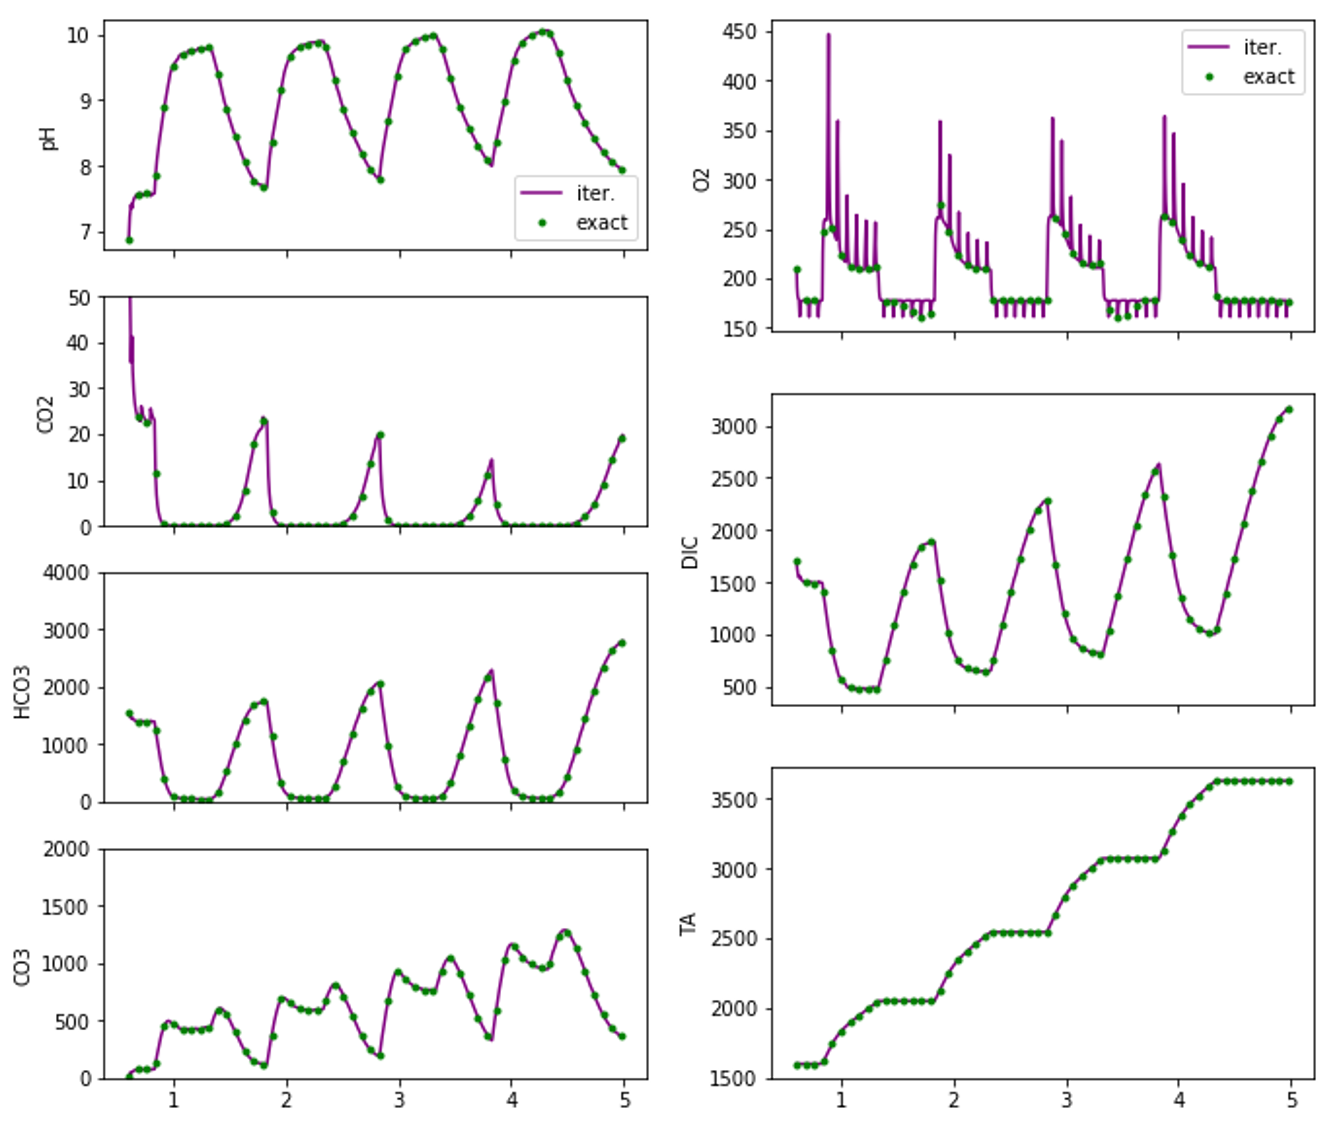
\includegraphics[width=0.9\textwidth]{images_microalgae/plots/iterative_carbon_and_states}}
	\caption[.]{Iterative (3rd iteration) vs exact solution for carbon chemistry $CO_2$, $HCO_3$, $CO_3$, $pH$ and state variables $O_2$, $DIC$, and $TA$.}
	\label{fig:iterative_carbon_and_states}
\end{figure}



\begin{table}
	\begin{tabular}{|c|c|c|c| c | c|} 
		\hline
		\bfseries{Variable} & \bfseries{Iter. 1} & \bfseries{Iter. 2} & \bfseries{Iter. 3}  &  \bfseries{Iter. 4} & \bfseries{Iter. 5} \\ \hline
		$pH$		& 0.036092734	&0.002355758	&1.41E-05		&6.93E-06		&6.93E-06 		\\
		$CO_2$		& 2.109401968	&0.145719349	&0.001222812	&0.000866728	&0.000866727 	\\
		$HCO_3$		& 19.81869214	&1.21021115		&0.008016765	&0.001025002	&0.001025139 	\\
		$CO_3$		& 20.89660704	&1.307061652	&0.00867642		&0.001102278	&0.001102434 	\\
		$DIC$		& 16.78775711	&0.958511825	&0.005229318	&0.002305054	&0.002333411 	\\
		$O_2$		&  0.308389964	&0.016044284	&4.18E-05		&6.89E-05		&7.59E-05 		\\
		$TA$		&  2.607767674	&0.160897272	&0.000688102	&0.001257725	&0.001218981 	\\
		\hline
	\end{tabular}
	\caption{RMSE for 5 iterations of the Newton-raphson carbon chemistry iterative solution.}
	\label{table:rmse_iterative}
\end{table}




%%
%% additional info
%%




%The CO2SYS Matlab version \cite{van2011matlab} was used to produce values of CO$_2$ and HCO$_3^-$ across DIC range 200-2500. 



% Total inorganic CO$_2$ (TCO$_2$) is the sum of the dissolved CO$_2$, the carbonate (CO$_{3-2}$), and the bicarbonate (HCO$_3^-$).



\FloatBarrier
\subsection{Process model: Gas transfer equilibrium concentrations for $O_2$ and $CO_2$}

%Weiss 1970 (O2) and 1974 (CO2) 

%\begin{equation}
%\begin{aligned}
%ln(Ko) =  A_{1} + A_{2}(100/T) + A_{3} ln(T/100) + S\% [B_{1} + B_{2}(T/100) + %B_{3}(T/100)^2 ] 
%\end{aligned}
%\end{equation}

The equilibrium concentration for CO$_2$ solubility in water $CO_{2H}$ ($\mu$mol/L) is calculated using Henry's law,
\begin{equation}\label{eq:CO2H_eq}
CO_{2H}=K0_{CO2}*fCO2*1.0220*1e6
\end{equation}
where fCO2 (atm) is the fugacity or approximately the partial pressure of CO$_2$, 1.0220 is the density of seawater (kg/L) at salinity 34 ppt and temperature 27$^{\circ}$C \cite{ramsing2011seawater} \cite{greensberg1992standard}. K0$_{CO2}$ (mol/kg$_{soln}$/atm) is the solubility of gas in seawater and is calculated from the fitted van't Hoff equation and the logarithmic Setchenow salinity dependence \cite{weiss1974carbon},
\begin{equation}
\begin{aligned}
K0_{CO2} = e^{(- 60.2409 + 93.4517\frac{100}{T_K}  + 23.3585*log(\frac{T_K}{100})+ 
S(0.023517 - 0.023656\frac{T_K}{100} + 0.0047036(\frac{T_K}{100})^2))}
\end{aligned}
\end{equation}
where $T_K$ is the temperature (K) and $S$ is salinity (ppt).
%% from Weiss 1974 paper:
%K0 may be expressed either in moles/1 * atm, referring to a liter of solution at %the temperature of the measurement and an atmosphere fugacity in
%the gas phase, or in moles/kg * atm, referring to a kilogram of solution.
Similarly the equilibrium concentration for $O_2$ solubility in water $O_{2H}$ is calculated using Henry's law,
\begin{equation}\label{eq:O2H_eq}
O_{2H}=K0_{O2}*fO2*1.0220*1e-6
\end{equation}
where fO2 (atm) is the fugacity or approximately the partial pressure of $O_2$, 1.0220 is the density of seawater (kg/L) at salinity 34 ppt and temperature 27$^{\circ}$C \cite{ramsing2011seawater} \cite{greensberg1992standard}, and K0$_{O2}$ (mol/kg$_{soln}$/atm) is the solubility of oxygen in seawater with an adjusted salinity dependence \cite{battino1983solubility},
\begin{equation}
\begin{aligned}
K0_{O2} =  \frac{e^{(-1282.8704 + \frac{36619.96}{T_K} + 223.1396 log(T_K) -0.354707 T_K 
+ S(5.957e-3 -\frac{3.7353}{T_K}) + 3.68e-6 S^2)}}{0.2094e-6}
\end{aligned}
\end{equation}
where $T_K$ is the temperature (K) and $S$ is salinity (ppt).
%from Weiss 1970:
%\begin{equation}
%\begin{aligned}
%K0_{O2} = exp(- 58.3877 + 85.8079(100/T_K)  + 23.8439*ln(T_K/100) + \\
%S(-0.034892 + 0.015568(T_K/100) - 0.0019387(T_K/100)^2))
%\end{aligned}
%\end{equation}
The equilibrium concentrations for $O_2$ and $CO_2$ are modelled together with the gas turning on and off during the experiment, as
\begin{equation}
 Q^{air} kLa_{O_2}^{air} (O_{2H} - O_{2})
\end{equation}
\begin{equation}
 Q^{air} kLa_{CO_2}^{air} (CO_{2H} - CO_{2})
\end{equation}
where $Q^{air}$ is the gas state (1= on, 0= off), $kLa_{O_2}^{air}$ and $kLa_{CO_2}^{air}$ are the mass transfer coefficients for air (d$^{-1}$), and 0.893 is the ratio between measured $O_2$ and $CO_2$ mass transfer constants \cite{grima1993gas}.



\subsection{Process model: Flux into cells by photosynthesis and respiration}

The carbon flux into cells is measured by net photosynthesis,
\begin{align}
\frac{\partial DIC}{dt} &=&  -(P I \frac{HCO_3^-}{K_m + HCO_3^-}  - R) 
\\
\frac{\partial O_2}{dt}	&=&  \frac{1}{(RQ_d I + RQ_n(1-I))}(P I \frac{HCO_3^-}{K_m + HCO_3^-}  - R)
\\
\frac{\partial TA}{\partial t}  &=&      R_R (P I \frac{HCO_3^-}{K_m + HCO_3^-}) \phantom{- R)}
\\
\frac{\partial C_p}{\partial t} &=& 	 (P I \frac{HCO_3^-}{K_m + HCO_3^-} - R) 
\\\nonumber
\end{align} 
where the parameters common to all states are $P$, the maximum photosynthesis rate ($\mu$M L$^{-1}$ hour$^{-1}$), $I$ the light indicator (0/1), and the michaelis menton term $\frac{HCO_3^-}{K_m + HCO_3^-}$ representing the photosynthetically active carbon used for photosynthesis. This can be $CO_2$, $HCO_3^-$, or a combination of both, $CO_2 + HCO_3^-$ if the microalgae are using both carbon dioxide and bicarbonate for photosynthesis. $K_m$ is the carbon restriction term ($\mu$M L$^{-1}$).

The respiration rate $R$ ($\mu$M L$^{-1}$ hour$^{-1}$), is present in the net photosynthesis calculation for dissolved inorganic carbon ($DIC$), oxygen ($O_2$), and carbon concentration in the form of cells ($C_p$). Oxygen also accounts for the day ($RQ_d$) and night respiratory quotients ($RQ_n$), the ratio of $CO_2$ produced and $O_2$ consumed by a cell. 
Total alkalinity ($TA$) only increases due to photosynthesis while accounting for the Redfield ratio ($R_R$).

%$RQ_d$ and $RQ_n$ are the day and night respiratory quotients, the ratio of $CO_2$ produced and $O_2$ consumed by a cell. 

%$C_p$ is the amount of carbon in the PBR in the form of cells, it is the same amount as the photosynthesis term in the DIC state. it is also subject to dilution. The aim of including this is the first step towards quantifying the biomass. later you can build in light etc 


[BM: Chris do I need more explanation here? Or references?]

\subsection{Process model: Dilution}

To maintain a semi-batch culturing system, manual dilutions that occurred once per day over the period of the experiment were extracted to measure total alkalinity and dissolved inorganic carbon (described in more detail in Section \ref{sec:micro_data_collection}). This also keeps the algae in the growth stage of the biomass curve, resetting it every day so that it never reaches the logit plateau. In the ODE's this affects every state variable, dissolved organic carbon ($DIC$), oxygen ($O_2$), total alkalinity ($TA$) and amount of carbon in the form of cells ($C_p$),
\begin{align}
\frac{\partial DIC}{dt} &=&   \frac{Q^M}{V}(DIC^{M} - DIC) 
\\
\frac{\partial O_2}{dt}	&=&   \frac{Q^M}{V}(\phantom{C}O_{2}^{M} - \phantom{CC}O_{2})
\\
\frac{\partial TA}{\partial t}  &=&  \frac{Q^M}{V}(\phantom{C}TA^{M} - \phantom{C}TA)
\\
\frac{\partial C_p}{\partial t} &=&  \frac{Q^M}{V}(\phantom{CTA^{M}} - \phantom{IC}C_p)
\\\nonumber
\end{align} 
where $Q ^{M}$ is the measured dilution rate (ml day$^{-1}$) used to force the model, $V$ is the volume of the photo-bioreactor fixed at 500$\mskip3mu$ml, and $DIC ^{M} $, $O_2^{M}$, and $TA^{M}$ are the respective concentrations of the media.
The media concentrations were calculated using CO2SYS (at temperature = 27 and salinity = 34) and set to be fixed throughout the experiment as $DIC ^{M} $= 1724.20$\mskip3mu$$\mu$M L$^{-1}$, $O_2^{M}$ = 226.65$\mskip3mu$$\mu$M L$^{-1}$, and $TA^{M}$ = 1797.90$\mskip3mu$$\mu$M L$^{-1}$.



\subsection{Process model summary and parameter model}\label{sec:micro_process_model}

A summary of the ODE's that make up the process model described in previous sections:
\begin{align}
\text{Rate} & & \text{flux into cells}            &            &\text{gas transfer}   &     & \text{dilution} \nonumber                              \\
\frac{\partial DIC}{\partial t}&=&                      - (P I \frac{HCO_3^-}{K_m + HCO_3^-} - R)&      &+\hat Q^{air}kLa_{ CO_2}^{air}(CO_{2}^{air} - CO_{2})                  & &+\frac{Q^M}{V}(DIC^{M} - DIC)       \nonumber \\
%                                           &  &                                   &      &+\hat Q^{co2}kLa_{ CO_2}^{co2}(CO_{2}^{co2} - CO_{2})    \\
\frac{\partial O_2}{\partial t}&=& \frac{(P I \frac{HCO_3^-}{K_m + HCO_3^-} - R)}{(RQ_d I + RQ_n(1-I))}  &      &+\hat Q^{air}kLa_{\phantom{C}O_2}^{air}(\phantom{C}O_{2}^{air} - \phantom{I}O_{2}) && +\frac{Q^M}{V}(\phantom{C}O_{2}^{M} - \phantom{CC}O_{2})     \nonumber   \\
 %                                          &  &                                   &      &+\hat Q^{co2}kLa_{\phantom{C}O_2}^{co2}(\phantom{C}O_{2}^{co2} - \phantom{C}O_{2})    \\
\frac{\partial TA}{\partial t} & =&      R_R (P I \frac{HCO_3^-}{K_m + HCO_3^-} \phantom{ + R})& & & & +\frac{Q^M}{V}(\phantom{C}TA^{M} - \phantom{I}TA) \nonumber\\
\frac{\partial C_p}{\partial t} & =& (P I \frac{HCO_3^-}{K_m + HCO_3^-} - R)&  & & & +\frac{Q^M}{V}(\phantom{CTA^{M}} - \phantom{II}C_p) 
\end{align}



\begin{longtable}{|c|c|l|c|l|}
	\hline 
	& Symbol & Description  & Prior / Value & Unit \\
    \hline
    \multirow{4}{*}{\rotatebox[origin=c]{90}{Initial conditions}}
    & $DIC^0$ & Dissolved inorganic carbon & Log$\mathcal{N}$(log(1300), 0.2) & $\mu$M L$^{-1}$ \\
    & $O_2^0$ & Oxygen & Log$\mathcal{N}$(log(225), 0.2) & $\mu$M L$^{-1}$ \\
    & $TA^0$  & Total alkalinity & Log$\mathcal{N}$(log(1750), 0.1) & $\mu$M L$^{-1}$ \\
    & $C_p^0$  & Carbon in the form of cells & Log$\mathcal{N}$(log(300), 0.2) & $\mu$M L$^{-1}$ \\
%    & $P^0$  & Rate of photosynthesis & & $\mu$M L$^{-1}$ day$^{-1}$\\
%    & $R^0$  & Rate of respiration & & $\mu$M L$^{-1}$ day$^{-1}$\\
    & $pH^0$ & -  & Log$\mathcal{N}$(log(8.5), 0.2) & log$_{10}$(-mol/L H+)  \\
    & $CO_2$$^0$ & Carbon dioxide  & Log$\mathcal{N}$(log(5), 0.4) & $\mu$M L$^{-1}$ \\
    & $HCO_3^-$$^0$ & Bicarbonate & Log$\mathcal{N}$(log(1500), 0.3) & $\mu$M L$^{-1}$  \\
    & $CO_3^{2-}$$^0$ & Carbonate & Log$\mathcal{N}$(log(100), 0.4) & $\mu$M L$^{-1}$ \\
    \hline
	\multirow{4}{*}{\rotatebox[origin=c]{90}{Flux into cells}}
	& $ P $ & Maximum photosynthesis rate  & * & $\mu$M L$^{-1}$ hour$^{-1}$ \\
	& $ R $ & Respiration rate & * & $\mu$M L$^{-1}$ hour$^{-1}$ \\ 
	& $ K_m $ & Carbon restriction & * & $\mu$M L$^{-1}$ \\
	& $ RQ_d $ & Daytime respiratory quotient & * & - \\
	& $ RQ_n $ & Night respiratory quotient & * & - \\
	& $ R_R $ & Redfield ratio & * & - \\
	& $ I $ & Light indicator & forcing (0/1) & - \\	
    \hline
    \multirow{4}{*}{\rotatebox[origin=c]{90}{Gas transfer terms }}
    & $ \hat Q ^{air} $ & Indicator for flow in air line  & forcing (0/1) & - \\
    & $x_{CO_2}^{air} $ & Mole fraction of CO$_2$ atmosphere & 400 & ppm \\ 
    & $CO_{2H}$  & Equilibrium CO$_2$ concentration  & Eq. \ref{eq:CO2H_eq} & $\mu$M L$^{-1}$  \\
    & $CO_{2}^{air}$ & Sat CO$_2$ conc with atmosphere &   $x_{CO_2}^{air} CO_{2H}$ & \\
    & $kLa_{ CO_2}^{air}$ & Mass transfer coefficient for CO$_2$ & 0.893$kLa_{\phantom{C}O_2}^{air}$  & day$^{-1}$ \\
    
    & $x_{O_2}^{air} $ & Mole fraction of O$_2$ atmosphere& 0.2094 & atm \\ 
    & $\phantom{C}O_{2H}$  & Equilibrium O$_2$ concentration  & Eq. \ref{eq:O2H_eq} & $\mu$M L$^{-1}$  \\
	& $\phantom{C}O_{2}^{air}$ & Sat O$_2$ conc with atmosphere &   $x_{O_2}^{air} O_{2H}$ & \\
    & $\tau$ & half-life of $kLa_{\phantom{C}O_2}^{air}$  & range(2-20) & min$^{-1}$\\
    & $kLa_{\phantom{C}O_2}^{air}$ & Mass transfer coefficient for O$_2$ & $\ln(2) * 24*60/\tau$ & day$^{-1}$\\
   
    \hline
        \multirow{4}{*}{\rotatebox[origin=c]{90}{Dilution terms }}
    &$  Q ^{M} $ & Dilution rate  & forcing & ml day$^{-1}$ \\
    &$  V $ & Volume of the reactor  & 500 & ml \\
    &$  DIC ^{M} $ & Media dissolved inorganic carbon  & 1724.20 & $\mu$M L$^{-1}$ \\ 
    &$	\phantom{CC}O_2^{M}$ & Media oxygen concentration & 226.65 & $\mu$M L$^{-1}$ \\
    &$	\phantom{C}TA^{M}$  & Media total alkalinity & 1797.90 & $\mu$M L$^{-1}$
    \\
    
        \hline
%    \multirow{4}{*}{\rotatebox[origin=c]{90}{Other dilution terms }}
%    &$ \hat Q ^{CO2} $ &indicator for dilution & 0 or 1 & - \\
%  
%    & $x_{\phantom{C}O_2}^{CO2} $ & mole fraction of & 0 & - \\ 
%    & $\phantom{C}O_{2}^{CO2}$ & sat CO$_2$ conc with CO$_2$ &   $x_{O_2}^{CO2} O_{2H}$ & \\
%    & $kLa_{ \phantom{C}O_2}^{CO2}$ & mass transfer coefficient &   & day$^{-1}$ \\
%    & $\phantom{C}O_2^{CO2}$  & & & \\
%    
%    & $x_{CO_2}^{CO2} $ & mole fraction of  & 1 & ppm \\ 
%    & $CO_{2}^{CO2}$ & sat CO$_2$ conc with CO$_2$ &   $x_{CO_2}^{CO2} CO_{2H}$ & \\
%    & $kLa_{ CO_2}^{CO2}$ & mass transfer coefficient & 0.893$kLa_{\phantom{C}O_2}^{CO2}$  & day$^{-1}$ \\
%    &$  CO_{2} ^{CO2} $ &   &  &  \\   
%    \hline
	\caption{State variable, parameter and forcing definitions with units, and their assignments: either fixed values, priors on initial condition or priors on parameters (*) defined later in respective sections.}
\end{longtable}  \label{tab:micro_parameter_model}
    



%\clearpage
%\begin{tabular}{l l  | l}
%	 \hline 
%	Symbol & Variable & Units  \\ \hline
%	DIC &  Dissolved inorganic carbon concentration & $\mu$mol/L  \\
%	O$_2$ & Oxygen  &  $\mu$mol/L \\
%	pH & -  & log$_{10}$(-mol/L H+)  \\
%	CO$_2$ & Carbon dioxide  & $\mu$mol/L \\
%	HCO$_3^-$ & Bicarbonate & $\mu$mol/L  \\
%	CO$_3^{2-}$ & Carbonate  & $\mu$mol/L \\
%	kLA$_{O2}$  & Mass transfer coefficient for O$_2$ &  d$^{-1}$  \\
%	
%	CO$_{2H}$  & Equilibrium CO$_2$ concentration  & $\mu$mols/L  \\
%	
%	K0$_{O2}$ &  Solubility of gas & mol/kg$_{soln}$/atm  \\
%	K0$_{CO2}$ & Solubility of gas & mol/kg$_{soln}$/atm   \\
%	TA  & Total alkalinity & $\mu$mols/L  \\
%	S  & Salinity &  ppt  \\
%	fCO2  & Fugacity/CO$_2$ partial pressure &  atm  \\
%	fO2  & Fugacity/O$_2$ partial pressure &  atm \\
%	
%	K$_m$ & Carbon restriction & $\mu$mols/L \\
%	
%	P & Photosynthesis rate & $\mu$mols/L/day \\
%	R & Respiration rate & $\mu$mols/L/day \\
%	R$_R$ & Redfield ratio & - \\	
%	R$_Q$ & Respiratory quotient & - \\
%\end{tabular}
%\captionof{table}{Table of variables and parameters.}

%\begin{tabular}{c c  | c}
%	 \hline
%	 Symbol & Variable & Units  \\ \hline
%	I &  Light Intensity  &  normalised to 0/1   \\
%	T & Temperature & $\circ$ C  \\
%	T$_K$ & Temperature &  K  \\
%	$\xi$ & gasflow &  on/off (1,0)  \\
%	
%\end{tabular}
%\captionof{table}{Table of Forcings}










\subsection{Design and setup of data assimilation model with both simulated and experimental data}

A simulated dataset was created by running the process model described in Section \ref{sec:micro_process_model} with a fixed set of parameters ($P$ = 200, $R$ = 30, $kLA_{O_2}^{air}$ = 200, $K_m$ = 150, $RQ_d$ = 0.85, $RQ_n$ = 0.95, $R_R$ = 0.075) and initial conditions ($O_2^0$ = 225, $DIC^0$ = 1250, $TA^0$ = 1750). 
Normally distributed noise was added to the simulated dataset with standard deviations of 2$\mskip3mu$$\mu$M L$^{-1}$  for $O_2$, 0.01 for $pH$ and 50$\mskip3mu$$\mu$M L$^{-1}$ for $DIC$ and $TA$.

The set of experimental runs with simulated observations are\\
1. All parameters constant through time.\\
2. P and R as random walks through time.\\
%3. Km is changing through time. [BM: maybe, might not work out]\\

The first set of results assimilated the simulated observations and tested how well the system recovered the true parameter values (Section \ref{sec:micro_sim_results1} and \ref{sec:micro_sim_results2}). Then the following results assimilated the experimental data with various formulations of model parameters (Section \ref{sec:micro_exp_results1} and \ref{sec:micro_exp_results2}). [BM: update these to their ref labels to reference each section]

The set of experimental runs with experimental data are\\
1. All parameters constant through time.\\
2. P and R as random walks through time.\\
3. P and R as random walks through time, with daily and nightly respiratory quotients as random walks through time. \\
4. Adding in an offset.\\
5. Thinning out the observations further.\\

%\subsection{Parameter Model: Priors} \label{sec:micro_parameter_model}
Each result section will include the treatment of parameters, priors and proposal distributions for clarity.  



\FloatBarrier
\section{Results}

State posteriors are visualised by plotting the median and shading 95\% credible intervals, while parameter priors and posteriors are displayed by histograms. Interval estimates (25\%, 75\%) and (5\%, 95\%) of parameter posterior distributions are also quoted. 
Where simulated data was assimilated the true parameter values are indicated by solid green lines.


%% for reference
%Approximating equations in place of CO2SYS:
%
%\begin{equation}
%\begin{aligned}
%HCO_3^- = exp(16.262 + 0.0047081*DIC - 0.11922*T + 0.0050303*alk1 \\
%+ 1.7093*log(DIC) + 0.38048*log(S) - 3.7548*log(alk1)\\
%- 2.292e-5*DIC*T - 0.0032028*DIC*log(DIC) - 0.00015313*DIC*log(S)\\
%+ 0.0032527*DIC*log(alk1) +\\ 0.021965*T*log(alk1) - 0.00090344*alk1*log(DIC))
%\end{aligned}
%\end{equation}
%
%\begin{equation}
%\begin{aligned}
%CO_2 = exp(-486.84 - 0.070754*DIC - 0.25277*T - 0.20674*S - \\
%0.11627*alk1 + 78.274*log(DIC) + 72.147*log(alk1) - 2.9438e-5*DIC*T\\
% - 5.8841e-6*DIC*alk1 - 0.0040234*DIC*log(DIC) + 0.016172*DIC*log(alk1)\\
% - 0.02039*T*log(DIC) + 0.062452*T*log(alk1) + 0.029857*S*log(alk1) \\
% + 0.0031507*alk1*log(DIC) + 0.010398*alk1*log(alk1) \\
% - 11.192*log(DIC)*log(alk1))
%\end{aligned}
%\end{equation}
%
%\begin{equation}
%\begin{aligned}
%pH = 9.5803 - 0.0027089*DIC - 0.018089*T - 0.012068*S + 0.0016329*alk1\\
%+ 1.2706e-5*DIC*T + 4.6961e-7*DIC*alk1 - 9.2122e-6*T*alk1 - \\
%5.9777e-8*DIC**2 - 2.194e-7*alk1**2 
%\end{aligned}
%\end{equation}



%% For reference

%\begin{equation}
%HCO_3^- =  -818.0204 +   1.9388 DIC  +  0.0681alk  -0.0003 DIC alk
%\end{equation}
%
%\begin{equation}
%\begin{aligned}
%CO_2 = exp(-10.6788 +   0.0096 DIC +   0.1479 T +   0.0330 S  -0.0015 alk \\
%-6.2777e-05 DIC T   - 8.778e-07 DIC alk)
%\end{aligned}
%\end{equation}
%
%\begin{equation}
%\begin{aligned}
%pH = 12.26 -0.0030605 DIC -0.043752 T -0.013625 S+ 0.00011315 alk\\
%+ 1.3463e-05 DIC T + 5.2215e-07 DIC alk
%\end{aligned}
%\end{equation}


\FloatBarrier
\subsection{Posterior results with simulated data where photosynthesis and respiration are constant through time}\label{sec:micro_sim_results1}
% micro_iterative_fake_v2.bi

%\textbf{Parameter model:}\\
Parameters $P$, $R$, $kLA_{O_2}$, $K_m$, $R_R$, $RQ_d$, and $RQ_n$ were all treated as constant through time but unknown with prior distributions and proposal distributions defined in Table \ref{tab:micro_sim_priors}. The other model parameters were defined earlier in Table \ref{tab:micro_parameter_model}.
The data model assigned log normally distributed observation errors for each instrument (Section \ref{sec:micro_data_model}) with observation error standard deviation values cited in Table \ref{tab:micro_sim_priors}.

\begin{longtable}{| c | c  |  c |}
	\hline
	\bfseries{Parameter} & \bfseries{Prior} &  \bfseries{Proposal} \\ \hline
	$P$  		& Log$\mathcal{N}$(log(250.0), 0.8)  & Log$\mathcal{N}$(log($P_1$), 0.08)   \\
	$R$  		& Log$\mathcal{N}$(log(20.0), 0.8)   & Log$\mathcal{N}$(log($R_1$), 0.08)   \\
	$kLA_{O2}$  & Log$\mathcal{N}$(log(200.0), 0.3)  & Log$\mathcal{N}$(log($kLA_{O2}$), 0.03) \\
	$K_m$ 		&  Log$\mathcal{N}$(log(200.0), 0.6) & Log$\mathcal{N}$(log($K_m$), 0.06) \\
	$R_R$  		& Uniform(0, 0.2) &  Trun$\mathcal{N}$($R_R$, 0.01, lower = 0, upper = 0.2) \\
	$RQ_d$  	& Uniform(0.6, 1) &  Trun$\mathcal{N}$($RQ_d$, 0.005, lower = 0.6, upper = 1.0)\\
	$RQ_n$  	& Uniform(0.6, 1) &  Trun$\mathcal{N}$($RQ_n$, 0.005, lower = 0.6, upper = 1.0)\\
	$\sigma_{O_2}$ 	& 0.3 	& * \\
	$\sigma_{pH}$ 	& 0.3 	& * \\
	$\sigma_{DIC}$ 	& 0.3 	& * \\	
	\hline
	\caption[.]{Table of Parameters, their priors and proposal distributions (* indicates the parameter was held fixed).}
	\label{tab:micro_sim_priors}
\end{longtable}
 

\begin{figure}
	\centerline{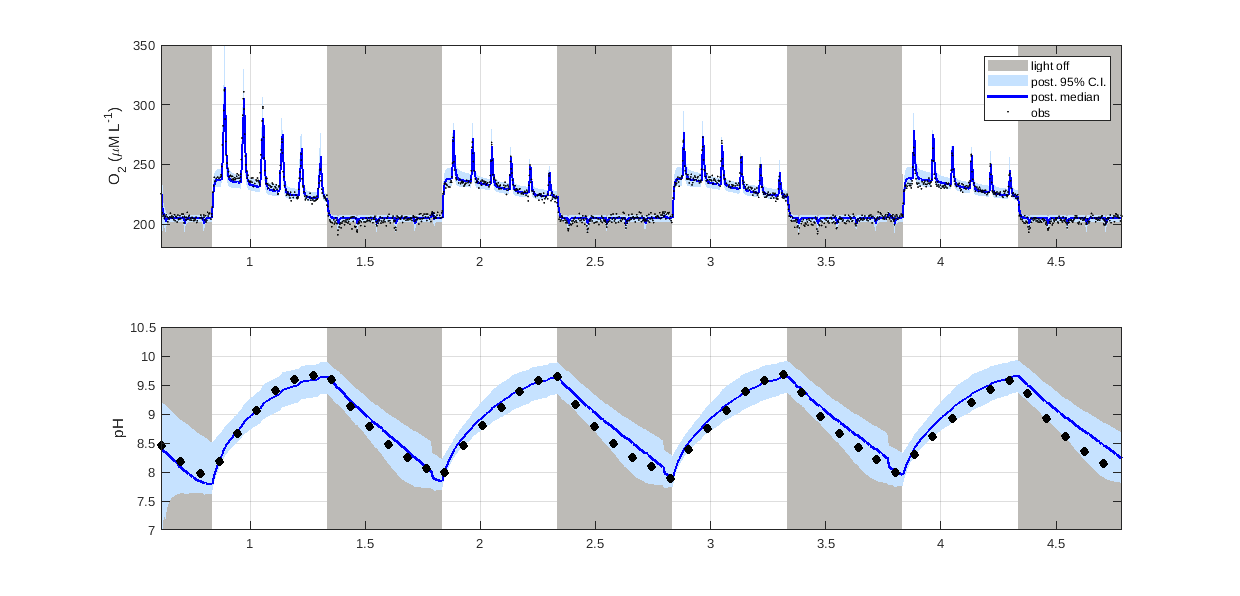
\includegraphics[width=1.2\textwidth]{images_microalgae/posterior_plots_with_fake_data/O2_pH}}
	\caption[.]{Posterior medians (solid blue line), 95\% credible intervals (shaded blue), and simulated observations (black) for $O_2$ and $pH$ across 4 days.}
	\label{fig:pos_sim_O2_pH}
\end{figure}

\begin{figure}
	\centerline{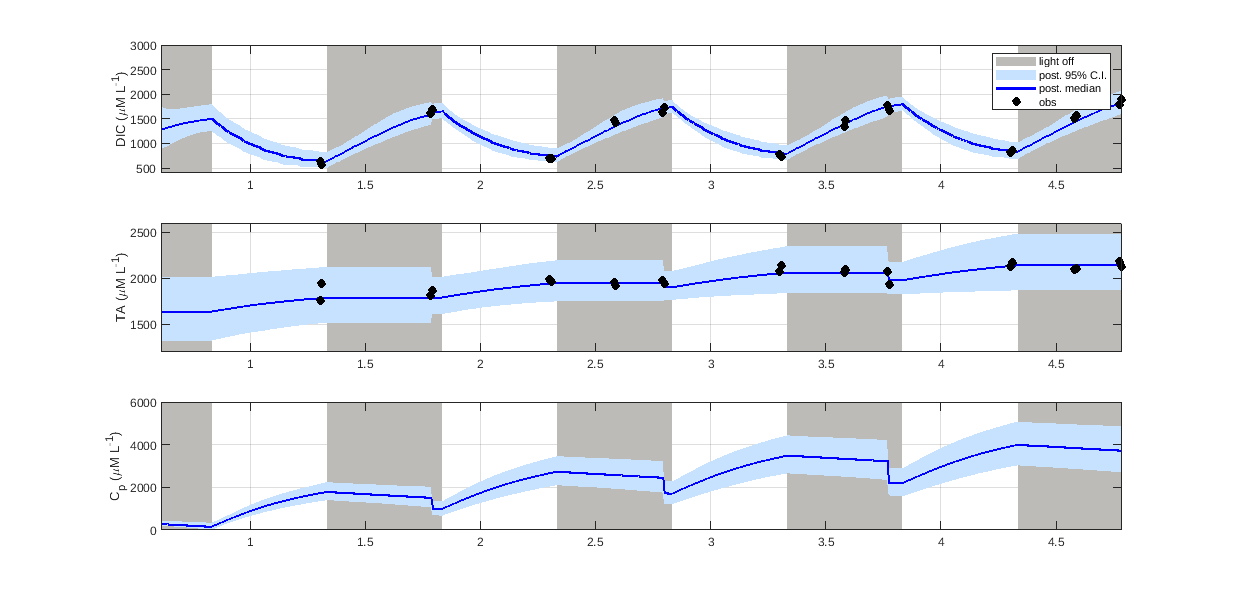
\includegraphics[width=1.2\textwidth]{images_microalgae/posterior_plots_with_fake_data/DIC_TA_Cp}}
	\caption[.]{Posterior medians (solid blue line), 95\% credible intervals (shaded blue), and simulated observations (black) for $DIC$, $TA$ and $C_p$ across 4 days.}
	\label{fig:pos_sim_DIC_TA_Cp}
\end{figure}

\begin{figure}
	\centerline{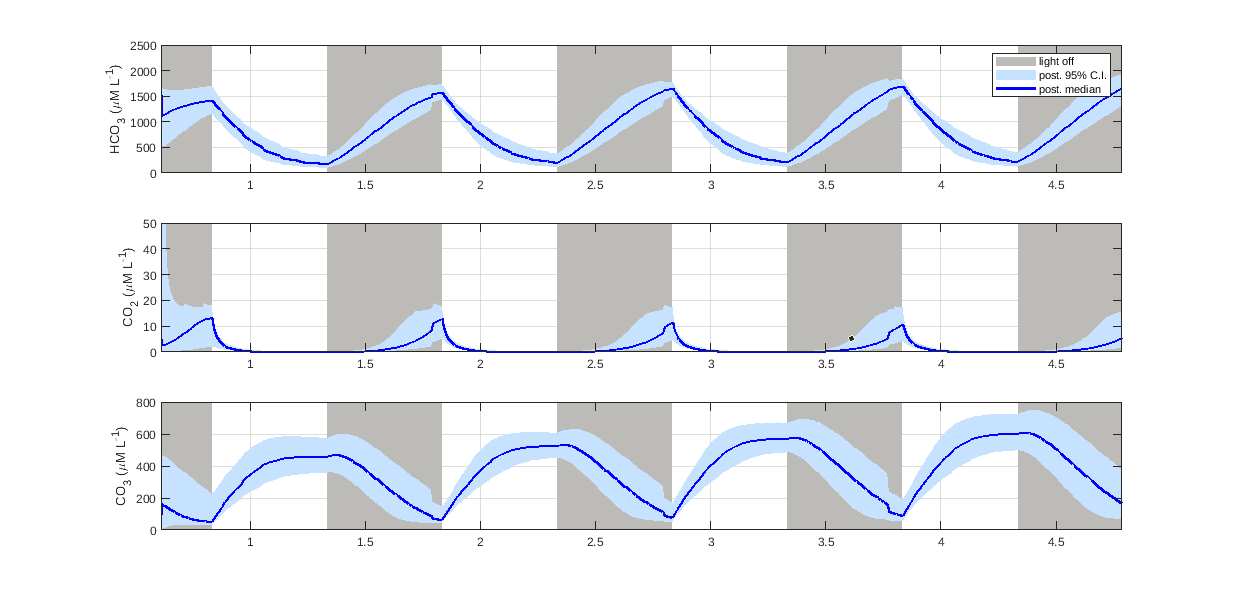
\includegraphics[width=1.2\textwidth]{images_microalgae/posterior_plots_with_fake_data/carbon}}
	\caption[.]{Posterior medians (solid blue line) and 95\% credible intervals (shaded blue) for $HCO_3$, $CO_2$ and $CO_3$ across 4 days.}
	\label{fig:pos_sim_carbon}
\end{figure}


\begin{figure}
	\centerline{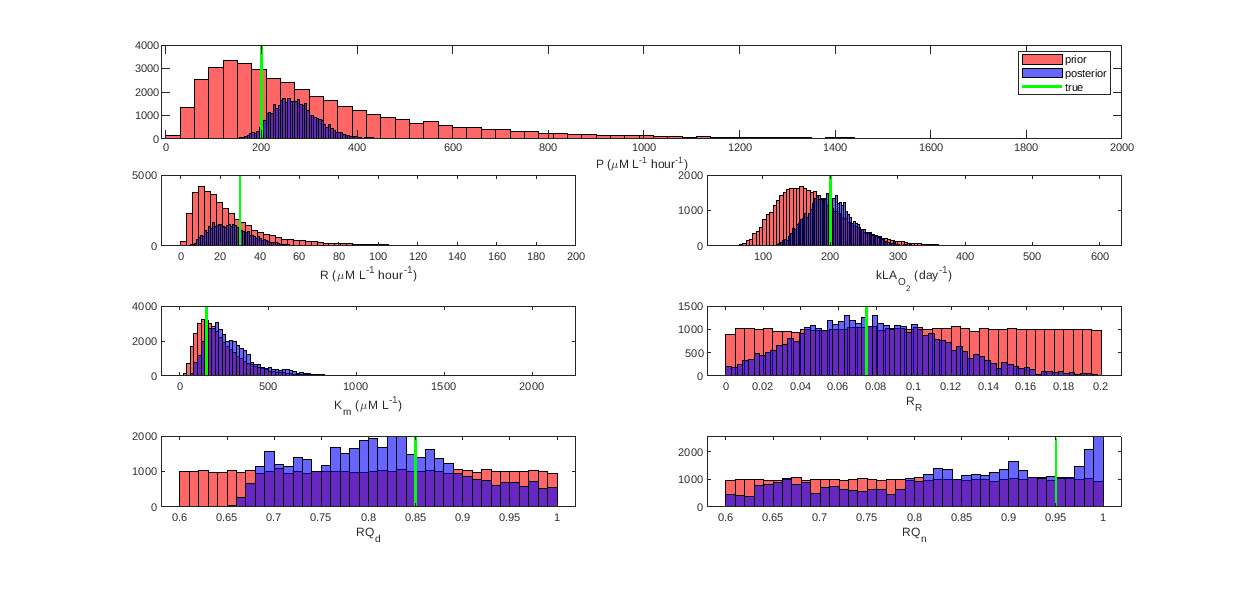
\includegraphics[width=1.3\textwidth]{images_microalgae/posterior_plots_with_fake_data/model_parameters}}
	\caption[.]{Priors (pink), posteriors (purple) and true values (green) for model parameters.}
	\label{fig:pos_sim_model_parameters}
\end{figure}


\begin{longtable}{|c|c|c|c|} 
		\hline
		\bfseries{Parameter}  & \bfseries{Quantiles (25\%, 75\%)}  & \bfseries{Quantiles (5\%, 95\%)} &  \bfseries{True value} \\ \hline
		$P$ 				& (237.2167, 302.0565) 	& (200.8971, 365.1751) 	&  200  \\ 
		$R$ 				& (17.5370, 32.3501) 	& (10.6537, 45.3096)	& 	30 \\ 
		$kLA_{O_2}^{air}$ 	& (177.1383, 222.9641)  & (148.2838, 267.5934)  &  200 \\
		$K_m$ 				& (182.6643, 362.6714) 	& (118.4125, 643.8518) 	&  150 \\ 
		$R_R$ 				& (0.0504, 0.1041) 		& (0.0196, 0.1458) 		& 0.075 \\
		$RQ_d$ 				& (0.7529, 0.8718) 		& (0.6894, 0.9666) 		& 0.85 \\	
		$RQ_n$ 				& (0.7469, 0.9338) 		& (0.6400, 0.9920) 		& 0.95 \\	
		\hline
		\caption[.]{True values for parameters used to create the simulated observations, and posterior (25\%, 75\%), (5\%, 95\%) quantiles for parameters after assimilating observations.}	
		\label{table:micro_parameters_sim}
\end{longtable}

%\textbf{Results:}\\
After running the PMMH for 50,000 samples (10,000 discarded as burn-in) with 1024 particles and tuning to an acceptance rate of 28.79\%, the true values of parameters $R$, $kLA_{O_2}^{air}$, $R_R$, and $RQ_d$ were recovered to the 25th and 75th percentile (Table \ref{table:micro_parameters_sim}, Figure \ref{fig:pos_sim_model_parameters}). While the true values of $K_m$ and $RQ_n$ did not lie within the 25th and 75th quantile, they were captured by the 5th and 95th percentiles (Table \ref{table:micro_parameters_sim}, Figure \ref{fig:pos_sim_model_parameters}). $P$ was the only parameter whose true value lied on the cusp of the 5th percentile. Parameters $P$, $R$, $kLA_{O_2}^{air}$, and $R_R$ mixed well, while parameters $K_m$, $RQ_d$, and $RQ_n$ did not mix as well, some autocorrelation between samples was present (Figure \ref{fig:micro_sim_model_parameters_traces}).

Observed state variables $O_2$, $DIC$, $TA$, and observed $pH$ posteriors were in excellent agreement with observations, with all observations fitting within the 95\% credible interval posteriors (Figure \ref{fig:pos_sim_O2_pH}, Figure \ref{fig:pos_sim_DIC_TA_Cp}).
Unobserved state variable posterior $C_p$ appeared to be constrained throughout the experiment (Figure \ref{fig:pos_sim_DIC_TA_Cp}). Similarly, the carbon chemistry variables $HCO_3$, $CO_2$, and $CO_3$ also had tightly constrained posteriors (Figure \ref{fig:pos_sim_carbon}).


% Log-likelihood stopped rising (Figure \ref{fig:micro_sim_loglikelihood}).


\FloatBarrier
\subsection{Posterior results with simulated data where photosynthesis and respiration are changing through time}\label{sec:micro_sim_results2}
% micro_iterative_fake.bi

Parameters $kLA_{O_2}$, $K_m$, $R_R$, $RQ_d$, and $RQ_n$ were all treated as constant through time but unknown with prior distributions and proposal distributions defined in Table \ref{tab:micro_sim_priors2}.
Photosynthesis ($P_1$) and respiration ($R_1$) were both modelled as random walks, by taking \begin{math}P\end{math} and \begin{math}R\end{math}, previously constant parameters, and replacing them by \begin{math}P_1(t)\end{math} and \begin{math}R_1(t)\end{math}. Here, we took \begin{math}P_1(t)\end{math} and \begin{math}R_1(t)\end{math} to be such that
\begin{displaymath}
P_1(t+\Delta t) = P(t) + r_P
\end{displaymath}
\begin{displaymath}
R_1(t+\Delta t) = R(t) + r_R
\end{displaymath}
where \begin{math}
r_P \sim N(0, \sigma_{r_P})
\end{math}, \begin{math}
r_R \sim N(0, \sigma_{r_R})
\end{math}, and \begin{math}
\Delta t
\end{math} is the length of discrete time-step. For the purpose of the Bayesian analysis here, \begin{math}\sigma_{r_P}\end{math} and \begin{math}\sigma_{r_R}\end{math} were treated as parameters to be inferred. 
The other model parameters were defined earlier in Table \ref{tab:micro_parameter_model}.
The data model assigned log normally distributed observation errors for each instrument (Section \ref{sec:micro_data_model}) with observation error standard deviation values cited in Table \ref{tab:micro_sim_priors2}.

\begin{longtable}{|c | c  |  c|}
	\hline
	\bfseries{Parameter} & \bfseries{Prior} &  \bfseries{Proposal} \\ \hline
	$kLA_{O2}$  & Log$\mathcal{N}$(log(200.0), 0.3)  & Log$\mathcal{N}$(log($kLA_{O2}$), 0.03) \\
	$K_m$ 		&  Log$\mathcal{N}$(log(200.0), 0.6) & Log$\mathcal{N}$(log($K_m$), 0.06) \\
	$R_R$  		& Uniform(0, 0.2) &  Trun$\mathcal{N}$($R_R$, 0.01, lower = 0, upper = 0.2) \\
	$RQ_d$  	& Uniform(0.6, 1) &  Trun$\mathcal{N}$($RQ_d$, 0.005, lower = 0.6, upper = 1.0)\\
	$RQ_n$  	& Uniform(0.6, 1) &  Trun$\mathcal{N}$($RQ_n$, 0.005, lower = 0.6, upper = 1.0)\\
	$\sigma_{r_P}$ & $\mathcal{N}$(0.01, 0.001)   & $\mathcal{N}$($\sigma_{r_P}$, 0.0001)   \\
	$\sigma_{r_R}$ & $\mathcal{N}$(0.01, 0.001)   & $\mathcal{N}$($\sigma_{r_R}$, 0.0001)   \\
	$\sigma_{O_2}$ 	& 0.3 	& * \\
	$\sigma_{pH}$ 	& 0.3 	& * \\
	$\sigma_{DIC}$ 	& 0.3 	& * \\	
	\hline
	\caption[.]{Table of Parameters, their priors and proposal distributions (* indicates the parameter was held fixed).}
	\label{tab:micro_sim_priors2}
\end{longtable}




\begin{figure}
	\centerline{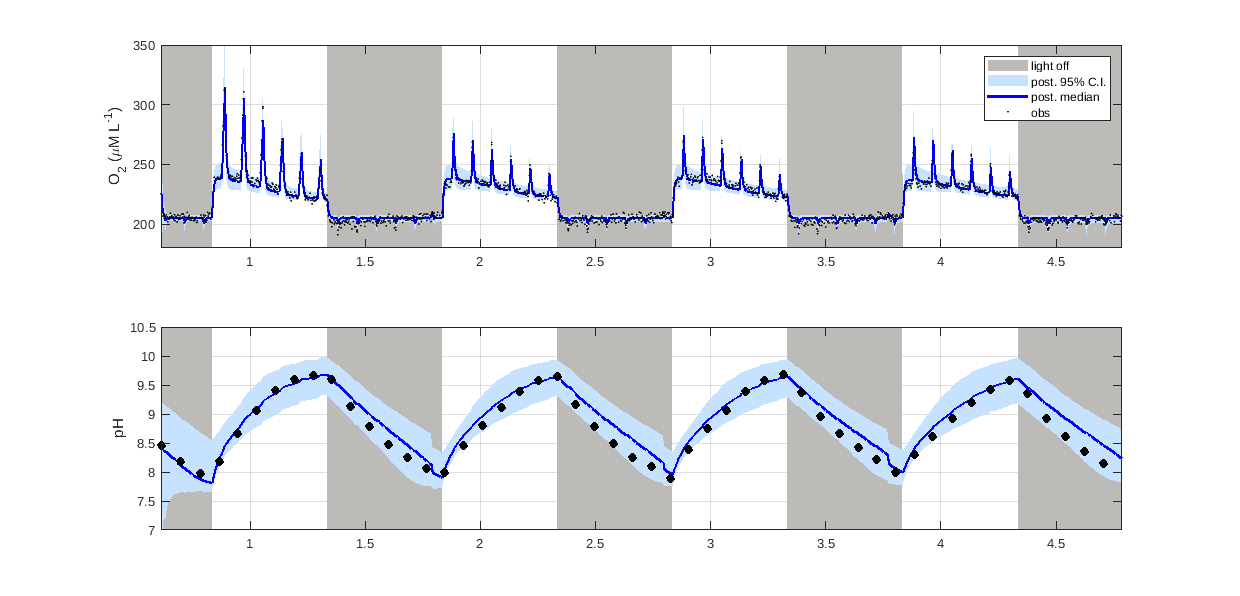
\includegraphics[width=1.2\textwidth]{images_microalgae/posterior_plots_with_fake_data_other/O2_pH}}
	\caption[.]{Posterior medians (solid blue line), 95\% credible intervals (shaded blue), and simulated observations (black) for $O_2$ and $pH$ across 4 days.}
	\label{fig:pos_sim_O2_pH_other}
\end{figure}

\begin{figure}
	\centerline{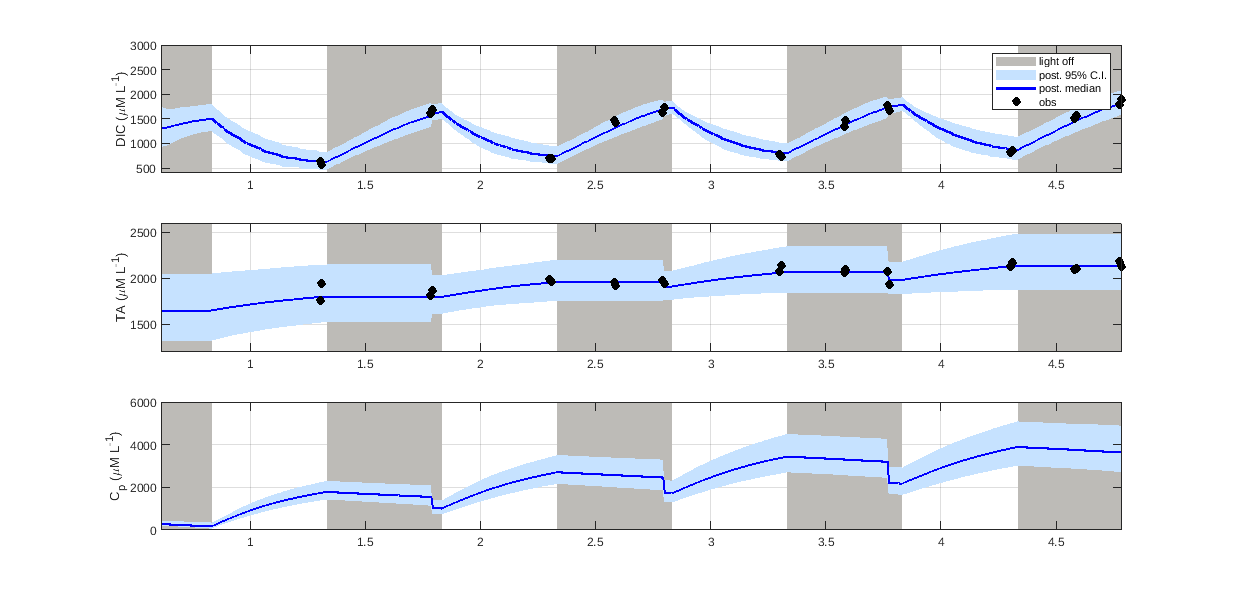
\includegraphics[width=1.2\textwidth]{images_microalgae/posterior_plots_with_fake_data_other/DIC_TA_Cp}}
	\caption[.]{Posterior medians (solid blue line), 95\% credible intervals (shaded blue), and simulated observations (black) for $DIC$, $TA$ and $C_p$ across 4 days.}
	\label{fig:pos_sim_DIC_TA_Cp_other}
\end{figure}

\begin{figure}
	\centerline{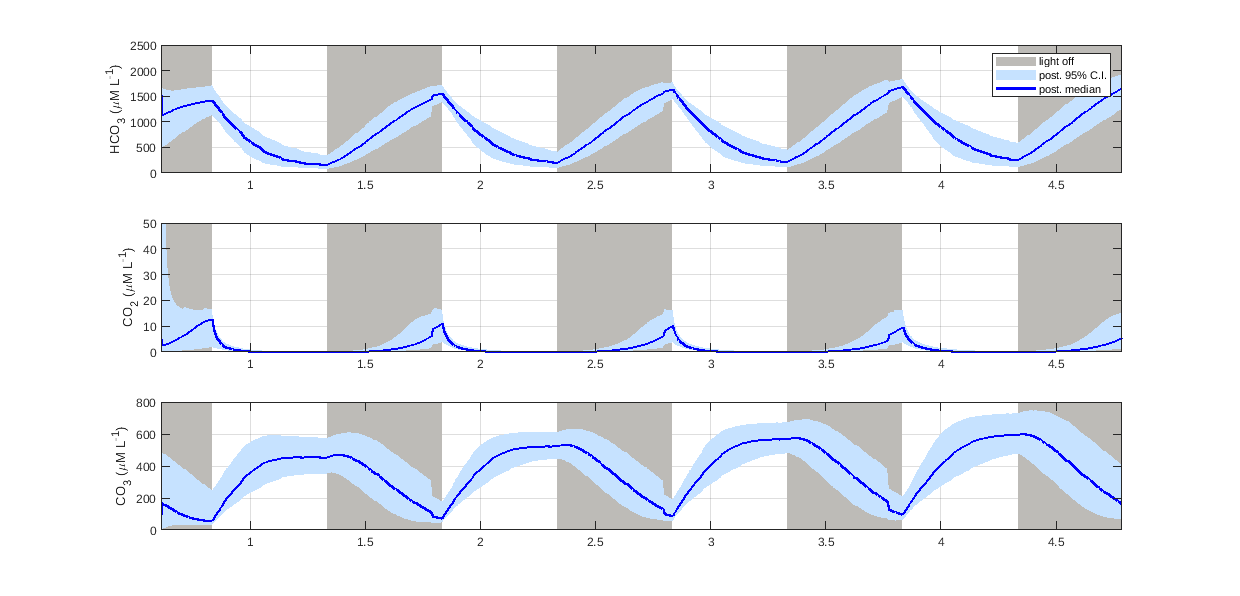
\includegraphics[width=1.2\textwidth]{images_microalgae/posterior_plots_with_fake_data_other/carbon}}
	\caption[.]{Posterior medians (solid blue line) and 95\% credible intervals (shaded blue) for $HCO_3$, $CO_2$ and $CO_3$ across 4 days.}
	\label{fig:pos_sim_carbon_other}
\end{figure}


\begin{figure}
	\centerline{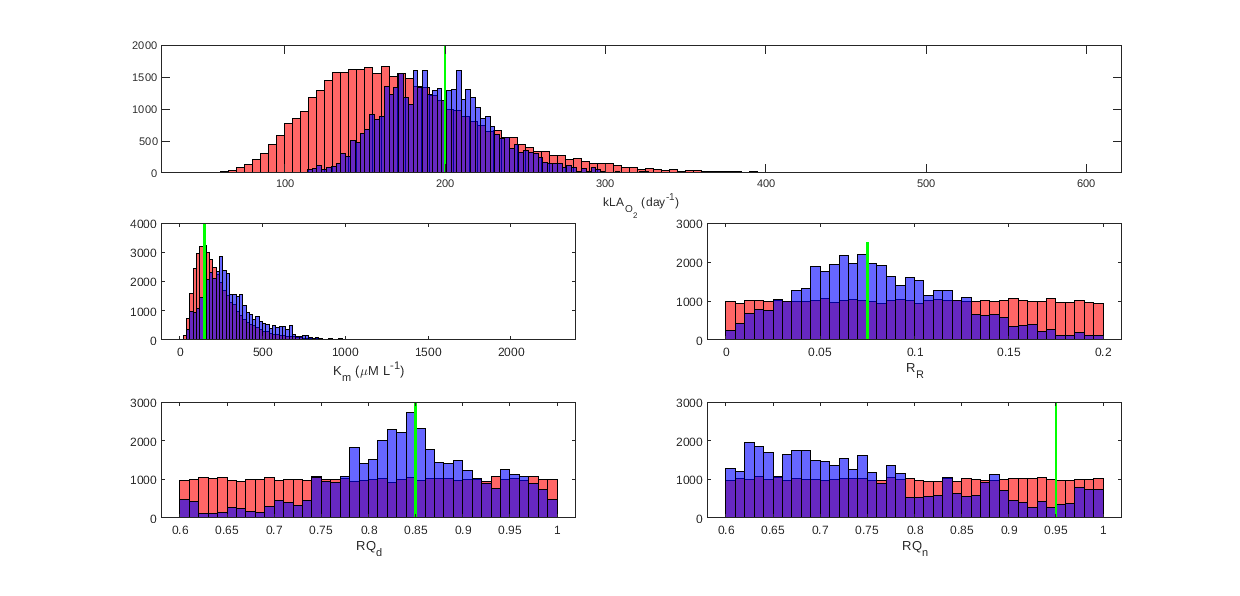
\includegraphics[width=1.3\textwidth]{images_microalgae/posterior_plots_with_fake_data_other/model_parameters}}
	\caption[.]{Priors (pink), posteriors (purple) and true values (green) for model parameters.}
	\label{fig:pos_sim_model_parameters_other}
\end{figure}

\begin{figure}
	\centerline{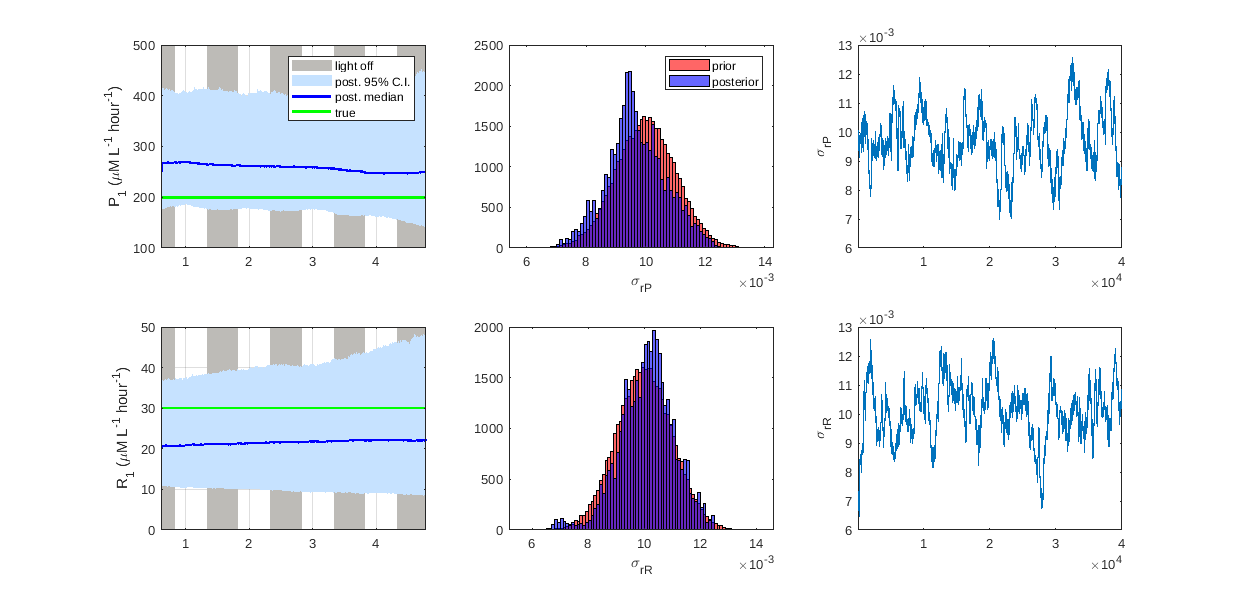
\includegraphics[width=1.3\textwidth]{images_microalgae/posterior_plots_with_fake_data_other/P_and_R}}
	\caption[.]{Random walk posteriors $P_1$ and $R_1$ medians (solid blue), 95\% credible intervals (shaded blue), and true values (green). $\sigma_{rP}$ and $\sigma_{rR}$ priors (pink), posteriors (purple), true values (green) and traces.}
	\label{fig:pos_sim_P_and_R_other}
\end{figure}

\begin{figure}
	\centerline{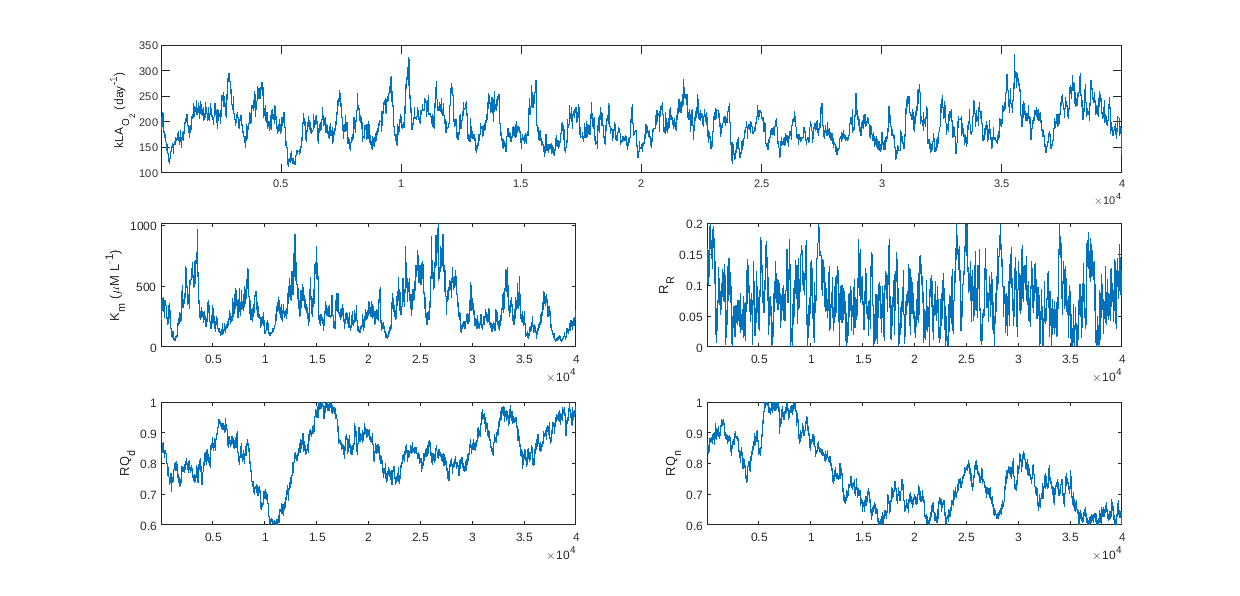
\includegraphics[width=1.3\textwidth]{images_microalgae/posterior_plots_with_fake_data_other/model_parameters_traces}}
	\caption[.]{Traces for model parameters.}
	\label{fig:micro_sim_model_parameters_other_trace}
\end{figure}

\begin{longtable}{|c|c|c|c|} 
	\hline
	\bfseries{Parameter}  & \bfseries{Quantiles (25\%, 75\%)}  & \bfseries{Quantiles (5\%, 95\%)} &  \bfseries{True value} \\ \hline
	$kLA_{O_2}^{air}$ 	& (170.9854, 216.0578)  & (145.6899, 253.4652)  &  200 \\
	$K_m$ 				& (187.3586, 386.4103) 	& (93.9670, 641.1432) 	&  150 \\ 
	$R_R$ 				& (0.0521, 0.1075) 		& (0.0192, 0.1544) 		& 0.075 \\
	$RQ_d$ 				& (0.7906, 0.8965) 		& (0.6833, 0.9711) 		& 0.85 \\	
	$RQ_n$ 				& (0.6654, 0.8334) 		& (0.6164, 0.9739) 		& 0.95 \\	
	\hline
	\caption[.]{True values for parameters used to create the simulated observations, and posterior (25\%, 75\%), (5\%, 95\%) quantiles for parameters after assimilating observations.}	
	\label{table:micro_parameters_sim_other}
\end{longtable}


After running the PMMH for 50,000 samples (10,000 discarded as burn-in) with 1024 particles and tuning to get an acceptance rate of 20.23\%, the true values of parameters $kLA_{O_2}^{air}$, $R_R$, and $RQ_d$ were recovered to the 25th and 75th percentile (Table \ref{table:micro_parameters_sim_other}). While the true values of $K_m$ and $RQ_n$ did not lie within the 25th and 75th quantile, they were captured by the 5th and 95th percentiles (Table \ref{table:micro_parameters_sim_other}). 
Parameters $\sigma_{rP}$, $\sigma_{rR}$, $kLA_{O_2}^{air}$, and $R_R$ mixed well, while parameters $K_m$, $RQ_d$, and $RQ_n$ did not mix as well, some autocorrelation between samples was present (Figure \ref{fig:micro_sim_model_parameters_other_trace}). The true values of $P_1$ (200) and $R_1$ (30) lay within the posterior 95\% credible intervals
(Figure \ref{fig:pos_sim_P_and_R_other}).
Observed state variables $O_2$, $DIC$, $TA$, and observed $pH$ posteriors were in excellent agreement with observations, with all observations fitting within the 95\% credible interval posteriors (Figure \ref{fig:pos_sim_O2_pH_other}, Figure \ref{fig:pos_sim_DIC_TA_Cp_other}).

Unobserved state variable posterior $C_p$ appeared to be constrained throughout the experiment (Figure \ref{fig:pos_sim_DIC_TA_Cp_other}).
Similarly, the carbon chemistry variables $HCO_3$, $CO_2$, and $CO_3$ also had tightly constrained posteriors (Figure \ref{fig:pos_sim_carbon_other}).



% Log-likelihood stopped rising (Figure \ref{fig:micro_sim_loglikelihood_other}).


\FloatBarrier
\subsection{Posterior results with experimental data where photosynthesis, respiration and respiratory quotients are changing through time}
% micro_iterative_chris.bi

Photosynthesis ($P_1$) and respiration ($R_1$) were both modelled as random walks as described in Section \ref{sec:micro_sim_results2}. 
Similarly, the respiratory quotients $RQ_d$ and $RQ_n$ were also treated as random walks, changing through time, with Wiener processes as standard deviations.
Parameters $kLA_{O_2}$, $K_m$, $R_R$, $\sigma_{rP}$, $\sigma_{rR}$ were all treated as constant through time but unknown with prior distributions and proposal distributions defined in Table \ref{tab:micro_priors_chris}.
The data model assigned log normally distributed observation errors for each instrument (Section \ref{sec:micro_data_model}) with observation error standard deviation values cited in Table \ref{tab:micro_priors_chris}.

\FloatBarrier
\begin{longtable}{|c | c  |  c|}
	\hline
	\bfseries{Parameter} & \bfseries{Prior} &  \bfseries{Proposal} \\ \hline
	$kLA_{O2}$  & Log$\mathcal{N}$(log(200.0), 0.3)  & Log$\mathcal{N}$(log($kLA_{O2}$), 0.03) \\
	$K_m$ 		&  Log$\mathcal{N}$(log(200.0), 0.6) & Log$\mathcal{N}$(log($K_m$), 0.06) \\
	$R_R$  		& Uniform(0, 0.2) &  Trun$\mathcal{N}$($R_R$, 0.005, lower = 0, upper = 0.2) \\
%	$RQ_d$  	& Uniform(0.6, 1) &  Trun$\mathcal{N}$($RQ_d$, 0.005, lower = 0.6, upper = 1.0)\\
%	$RQ_n$  	& Uniform(0.6, 1) &  Trun$\mathcal{N}$($RQ_n$, 0.005, lower = 0.6, upper = 1.0)\\
	$\sigma_{r_P}$ & $\mathcal{N}$(0.02, 0.002)   & $\mathcal{N}$($\sigma_{r_P}$, 0.0002)   \\
	$\sigma_{r_R}$ & $\mathcal{N}$(0.01, 0.001)   & $\mathcal{N}$($\sigma_{r_R}$, 0.0001)   \\
	$\sigma_{O_2}$ 	& 0.3 	& * \\
	$\sigma_{pH}$ 	& 0.3 	& * \\
	$\sigma_{DIC}$ 	& 0.5 	& * \\	
	\hline
	\caption[.]{Table of Parameters, their priors and proposal distributions (* indicates the parameter was held fixed).}
	\label{tab:micro_priors_chris}
\end{longtable}



\FloatBarrier
\begin{figure}
	\centerline{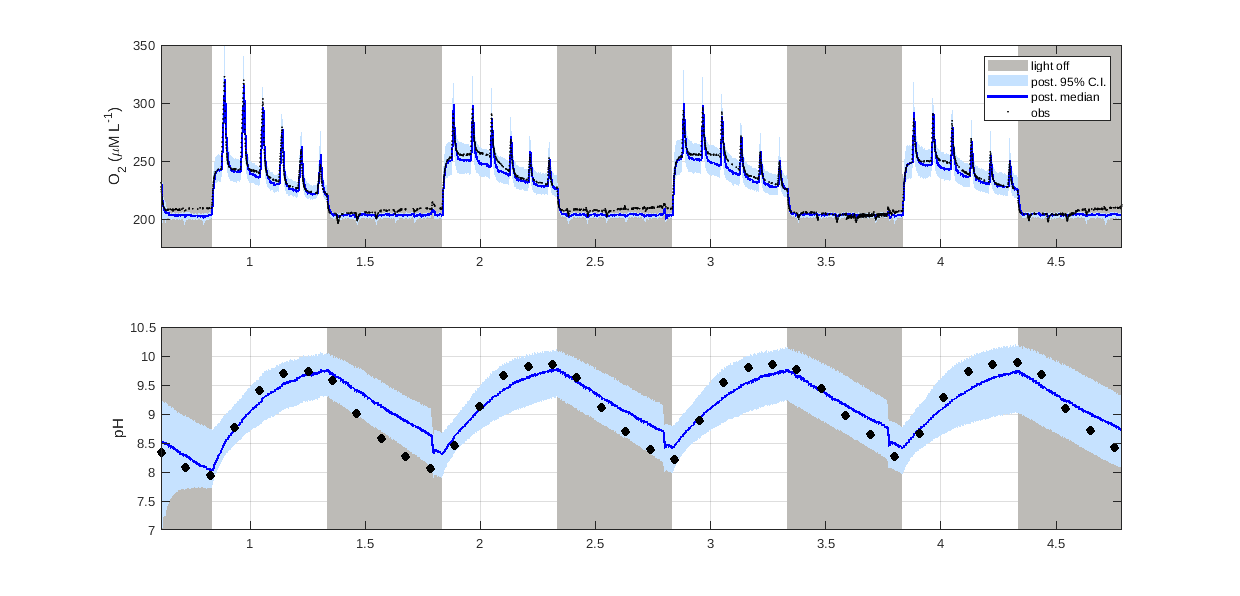
\includegraphics[width=1.2\textwidth]{images_microalgae/plots_chris/O2_pH}}
	\caption[.]{Posterior medians (solid blue line), 95\% credible intervals (shaded blue), and simulated observations (black) for $O_2$ and $pH$ across 4 days.}
	\label{fig:micro_exp_O2_pH}
\end{figure}

\begin{figure}
	\centerline{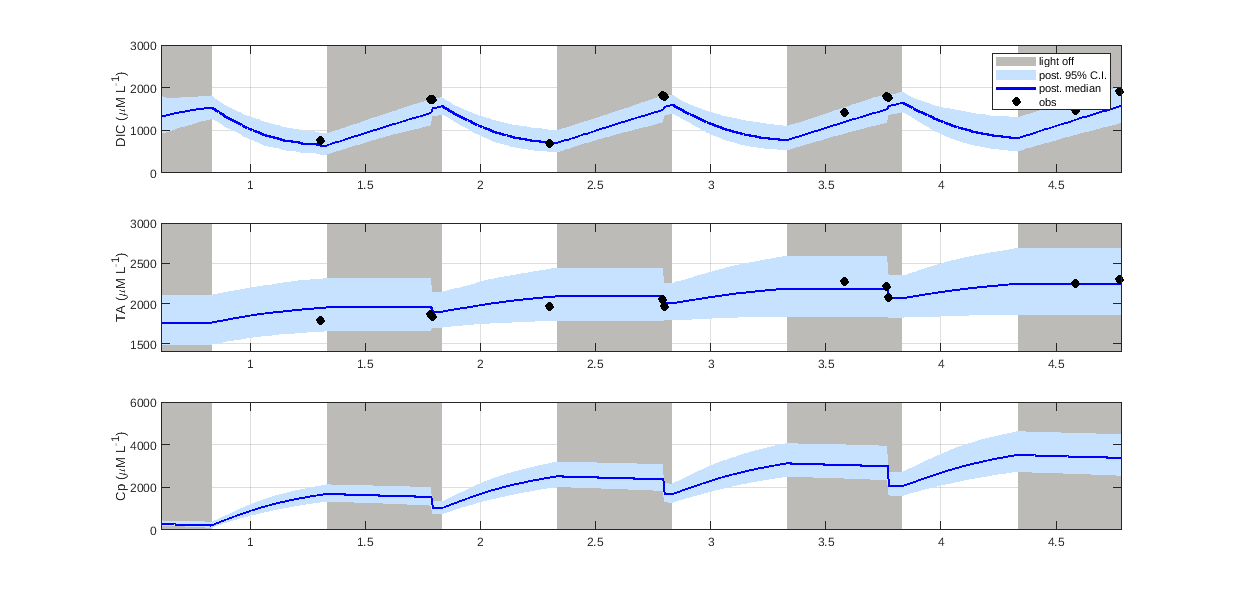
\includegraphics[width=1.2\textwidth]{images_microalgae/plots_chris/DIC_TA_Cp}}
	\caption[.]{Posterior medians (solid blue line), 95\% credible intervals (shaded blue), and simulated observations (black) for $DIC$, $TA$ and $C_p$ across 4 days.}
	\label{fig:micro_exp_DIC_TA_Cp}
\end{figure}

\begin{figure}
	\centerline{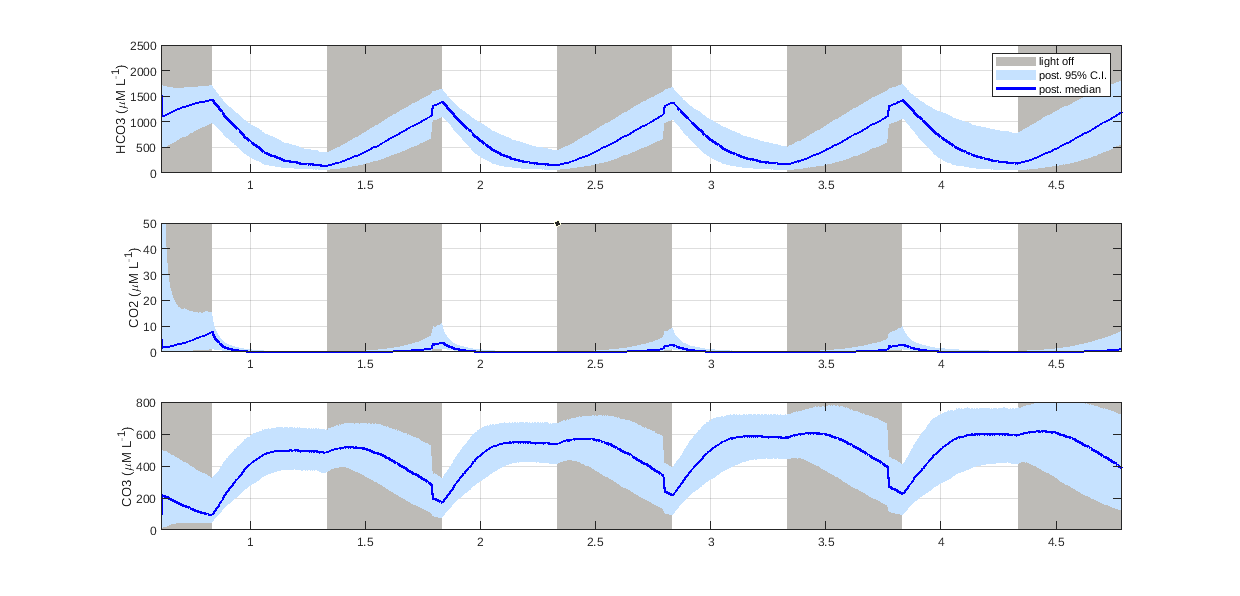
\includegraphics[width=1.2\textwidth]{images_microalgae/plots_chris/carbon}}
	\caption[.]{Posterior medians (solid blue line) and 95\% credible intervals (shaded blue) for $HCO_3$, $CO_2$ and $CO_3$ across 4 days.}
	\label{fig:micro_exp_carbon}
\end{figure}

\begin{figure}
	\centerline{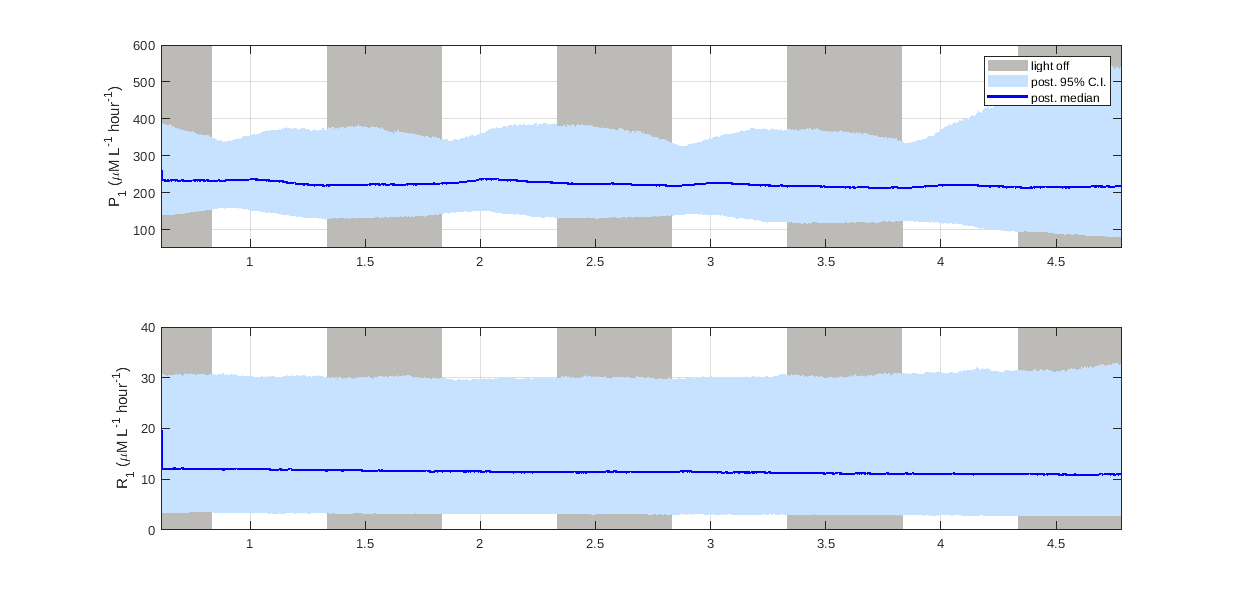
\includegraphics[width=1.2\textwidth]{images_microalgae/plots_chris/P_and_R}}
	\caption[.]{Posterior medians (solid blue line) and 95\% credible intervals (shaded blue) for photosynthesis $P_1$ and respiration $R_1$.}
	\label{fig:micro_exp_P_R}
\end{figure}

\begin{figure}
	\centerline{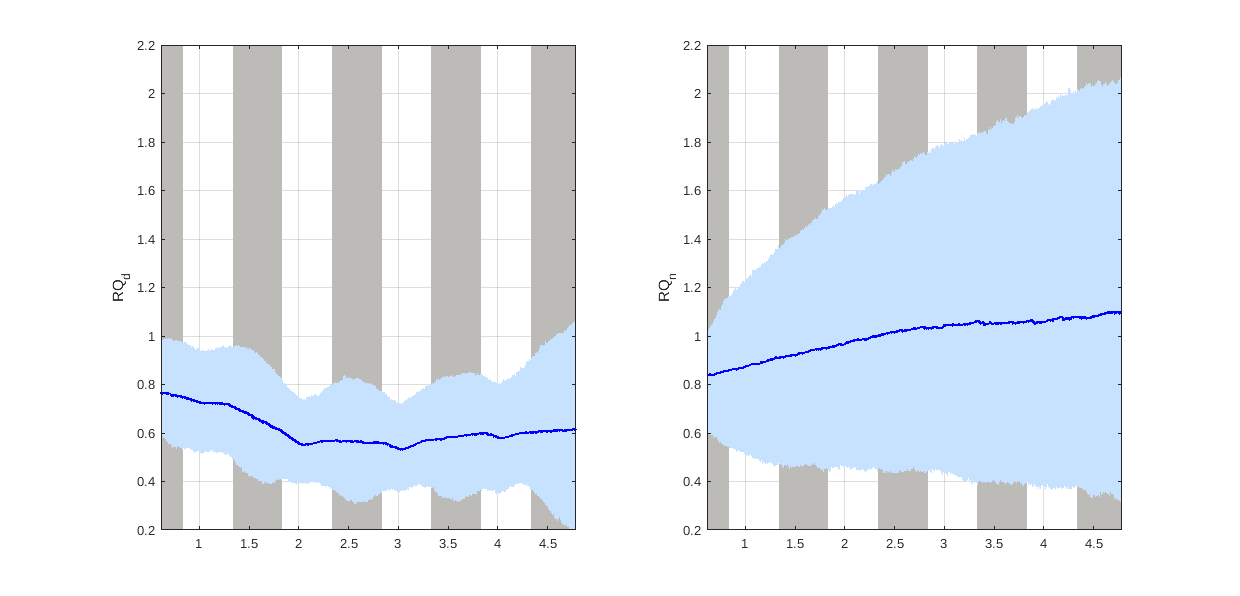
\includegraphics[width=1.2\textwidth]{images_microalgae/plots_chris/RQ_d_RQ_n}}
	\caption[.]{Posterior medians (solid blue line) and 95\% credible intervals (shaded blue) for $RQ_d$ and $RQ_n$.}
	\label{fig:micro_exp_RQ_d_RQ_n}
\end{figure}



\begin{figure}
	\centerline{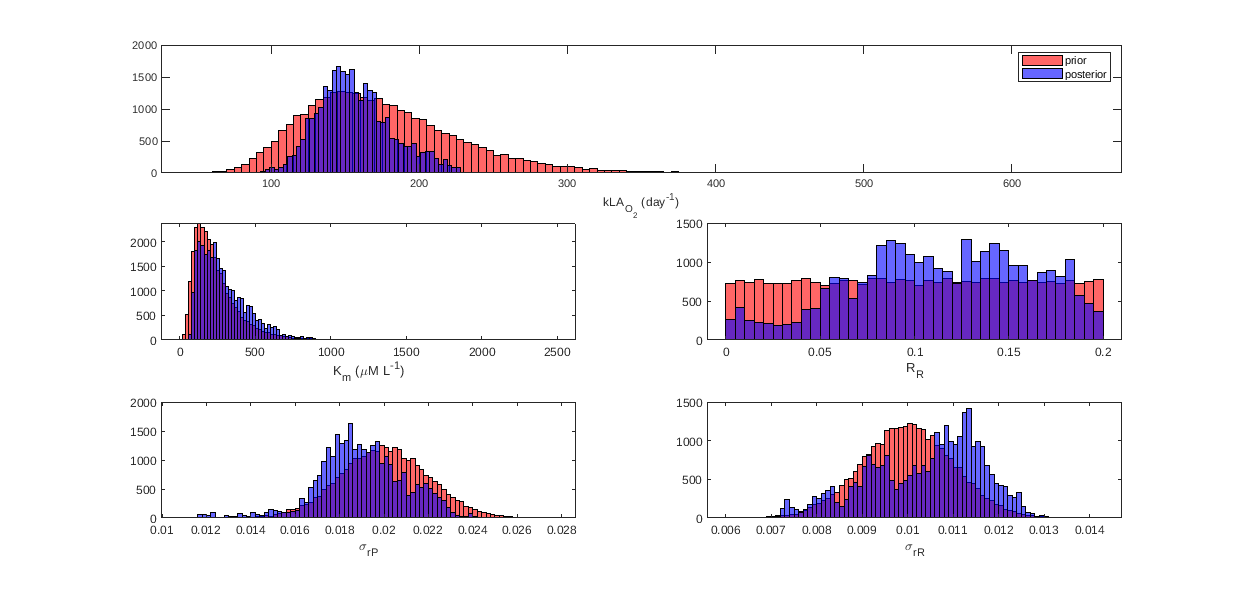
\includegraphics[width=1.3\textwidth]{images_microalgae/plots_chris/modelparameters1}}
	\caption[.]{Priors (pink) and posteriors (purple) for model parameters.}
	\label{fig:micro_exp_parameters_model}
\end{figure}

\begin{figure}
	\centerline{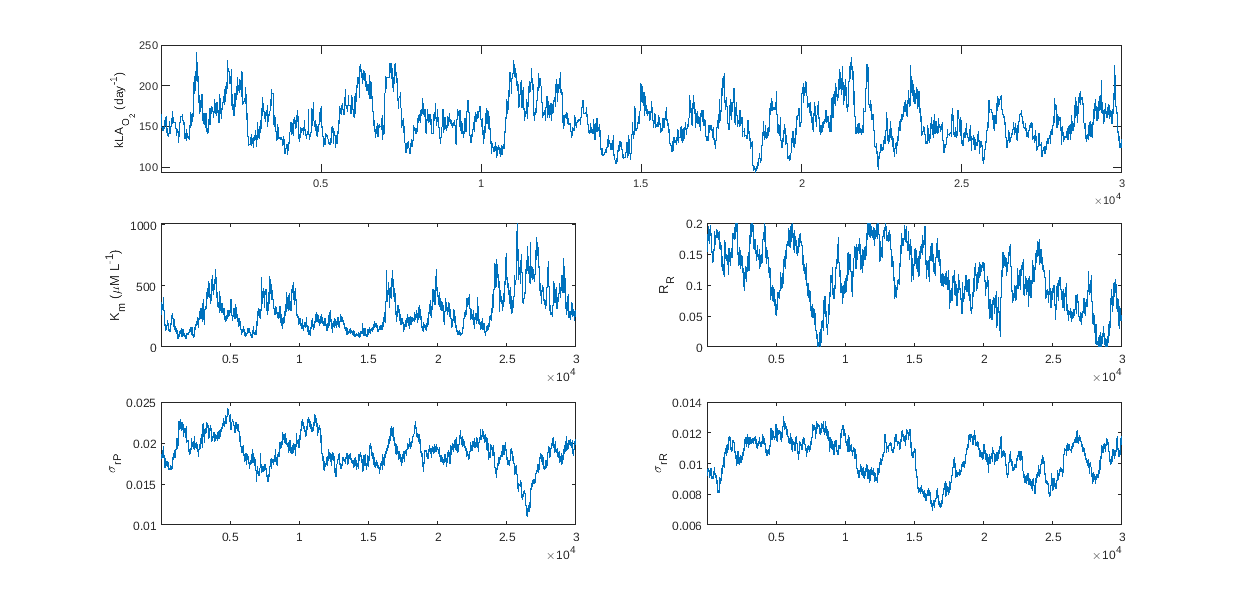
\includegraphics[width=1.3\textwidth]{images_microalgae/plots_chris/modelparameters1_trace}}
	\caption[.]{Traces for model parameters.}
	\label{fig:micro_exp_parameters_model2}
\end{figure}



\begin{longtable}{|c|c|c|} 
	\hline
	\bfseries{Parameter}  & \bfseries{Quantiles (25\%, 75\%)}  & \bfseries{Quantiles (5\%, 95\%)} \\ \hline
	$kLA_{O_2}^{air}$ 	& (139.5979, 170.8102)  & (120.9171, 204.5474)   \\
	$K_m$ 				& (168.1931, 378.8001) 	& (104.2598, 599.6881) 	 \\ 
	$R_R$ 				& (0.0815, 0.1512) 		& (0.0284, 0.1844) 		 \\
	$\sigma_{r_P}$ 		& (0.0178, 0.0202) 		& (0.0159, 0.0222) 		 \\ 
	$\sigma_{r_R}$ 		& (0.0094, 0.0113) 		& (0.0081, 0.0121)		 \\ 
	
	\hline
	\caption[.]{Posterior (25\%, 75\%), (5\%, 95\%) quantiles for parameters after assimilating observations.}	
	\label{table:micro_exp_parameters_table}
\end{longtable}

The PMMH was run for 40,000 samples with 1024 particles, where 10,000 samples were discarded as burn-in. 40,000 samples was all that could complete in the maximum time allocation on the hpc cluster.

Observed state variables $DIC$ and $TA$ posteriors perform well with all observations lying within the 95\% credible intervals (Figure \ref{fig:micro_exp_DIC_TA_Cp}). $O_2$ posteriors tracked the observations well while the light was on, with all observations falling inside tightly constrained 95\% credible intervals. During times when there was no light, most days the posteriors would fit the observations well to start and then potentially there was a sensor drift causing increasing observations that the model was not accounting for (Figure \ref{fig:micro_exp_O2_pH}). $pH$ captured most observations within the 95\% credible intervals except for 2 points on the 1st day while the light was off (Figure \ref{fig:micro_exp_O2_pH}).
 
The photosynthesis rate ($P_1$) centred around 240$\mskip3mu$$\mu$M L$^{-1}$ hour$^{-1}$ with small oscillations during daylight. The 95\% credible intervals lay approximately between 150$\mskip3mu$$\mu$M L$^{-1}$ hour$^{-1}$ and 400$\mskip3mu$$\mu$M L$^{-1}$ hour$^{-1}$ with tighter intervals at the start of each day (Figure \ref{fig:micro_exp_P_R}).
The respiration rate ($R_1$) remained centred around 12$\mskip3mu$$\mu$M L$^{-1}$ hour$^{-1}$ with 95\% credible intervals between 4$\mskip3mu$$\mu$M L$^{-1}$ hour$^{-1}$ and 30$\mskip3mu$$\mu$M L$^{-1}$ hour$^{-1}$ through the course of the experiment (Figure \ref{fig:micro_exp_P_R}).

The day-time respiratory quotient $RQ_d$ centred around 0.75 with a 95\% credible interval of 0.6-1 during the first day of the experiment. The centre dropped to 0.6 during the 2nd, 3rd and 4th days, with 95\% credible intervals of 0.4-0.8 (Figure \ref{fig:micro_exp_RQ_d_RQ_n}). The night-time respiratory quotient $RQ_n$ was initially centred around 0.85 and slowly rose to 1.1 by the end of the experiment. The 95\% credible intervals started with 0.6-1 and increased its span steadily to 0.4-2 by the end of the experiment (Figure \ref{fig:micro_exp_RQ_d_RQ_n}).

parameters

mixing

acceptance rate was 20.44\%.


[BM: Values $>$1 are not really realistic for respiratory quotients but this can be compensation for not having an offset on the $O_2$ obs, talk about this in the discussion]





\FloatBarrier
\subsection{Posterior results with experimental data where photosynthesis, respiration and respiratory quotients are changing through time and an offset on $O_2$ is introduced}\label{sec:micro_exp_offset}
% micro_iterative_chris_offset.bi


Photosynthesis ($P_1$) and respiration ($R_1$) were both modelled as random walks, by taking \begin{math}P\end{math} and \begin{math}R\end{math}, previously constant parameters, and replacing them by \begin{math}P_1(t)\end{math} and \begin{math}R_1(t)\end{math}. Here, we take \begin{math}P_1(t)\end{math} and \begin{math}R_1(t)\end{math} to be such that
\begin{displaymath}
P_1(t+\Delta t) = P(t) + r_P
\end{displaymath}
\begin{displaymath}
R_1(t+\Delta t) = R(t) + r_R
\end{displaymath}
where \begin{math}
r_P \sim N(0, \sigma_{r_P})
\end{math}, \begin{math}
r_R \sim N(0, \sigma_{r_R})
\end{math}, and \begin{math}
\Delta t
\end{math} is the length of discrete time-step. For the purpose of the Bayesian analysis here, \begin{math}\sigma_{r_P}\end{math} and \begin{math}\sigma_{r_R}\end{math} are treated as parameters to be inferred.  
The respiratory quotients $RQ_d$ and $RQ_n$ were also treated as random walks with $rP$ and $rR$ as wiener processes. 
Parameters $kLA_{O_2}$, $K_m$, $R_R$, $\sigma_{rP}$, $\sigma_{rR}$, and $offset_{O_2}$ were all treated as constant through time but unknown with prior distributions and proposal distributions defined in Table \ref{tab:micro_priors_chris_offset}.
The data model assigned log normally distributed observation errors for each instrument (Section \ref{sec:micro_data_model}) with observation error standard deviation values cited in Table \ref{tab:micro_priors_chris_offset}.

\FloatBarrier
\begin{longtable}{|c | c  |  c|}
	\hline
	\bfseries{Parameter} & \bfseries{Prior} &  \bfseries{Proposal} \\ \hline
	$kLA_{O2}$  & Log$\mathcal{N}$(log(200.0), 0.3)  & Log$\mathcal{N}$(log($kLA_{O2}$), 0.021) \\
	$K_m$ 		&  Log$\mathcal{N}$(log(200.0), 0.6) & Log$\mathcal{N}$(log($K_m$), 0.042) \\
	$R_R$  		& Uniform(0, 0.2) &  Trun$\mathcal{N}$($R_R$, 0.0035, lower = 0, upper = 0.2) \\
	%	$RQ_d$  	& Uniform(0.6, 1) &  Trun$\mathcal{N}$($RQ_d$, 0.005, lower = 0.6, upper = 1.0)\\
	%	$RQ_n$  	& Uniform(0.6, 1) &  Trun$\mathcal{N}$($RQ_n$, 0.005, lower = 0.6, upper = 1.0)\\
	$\sigma_{r_P}$ & $\mathcal{N}$(0.02, 0.002)   & $\mathcal{N}$($\sigma_{r_P}$, 0.00014)   \\
	$\sigma_{r_R}$ & $\mathcal{N}$(0.01, 0.001)   & $\mathcal{N}$($\sigma_{r_R}$, 0.00007)   \\
	$offset_{O_2}$ & $\mathcal{N}$(0, 5.0)     & $\mathcal{N}$($offset_{O_2}$, 0.5)   \\
	$\sigma_{O_2}$ 	& 0.1 	& * \\
	$\sigma_{pH}$ 	& 0.1 	& * \\
	$\sigma_{DIC}$ 	& 0.2 	& * \\
	\hline
	\caption[.]{Table of Parameters, their priors and proposal distributions (* indicates the parameter was held fixed).}	
	\label{tab:micro_priors_chris_offset}
\end{longtable}




\FloatBarrier
\begin{figure}
	\centerline{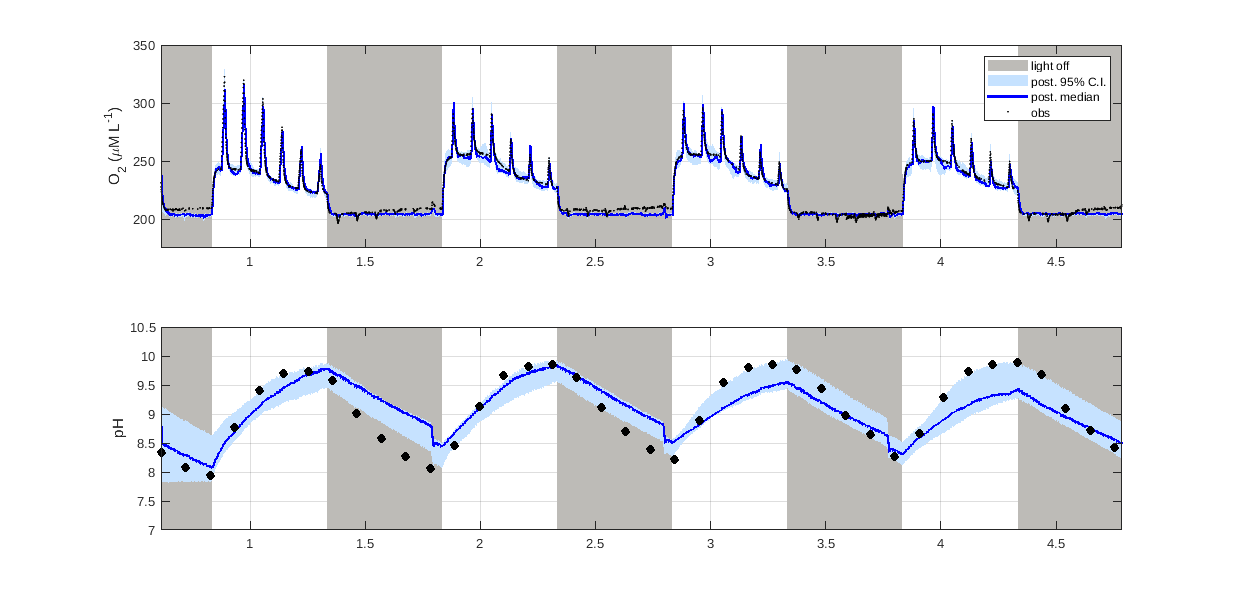
\includegraphics[width=1.2\textwidth]{images_microalgae/plots_chris_offset/O2_pH}}
	\caption[.]{Posterior medians (solid blue line), 95\% credible intervals (shaded blue), and observations (black) for $O_2$ and $pH$ across 4 days.}
	\label{fig:micro_exp_offset_O2_pH}
\end{figure}

\begin{figure}
	\centerline{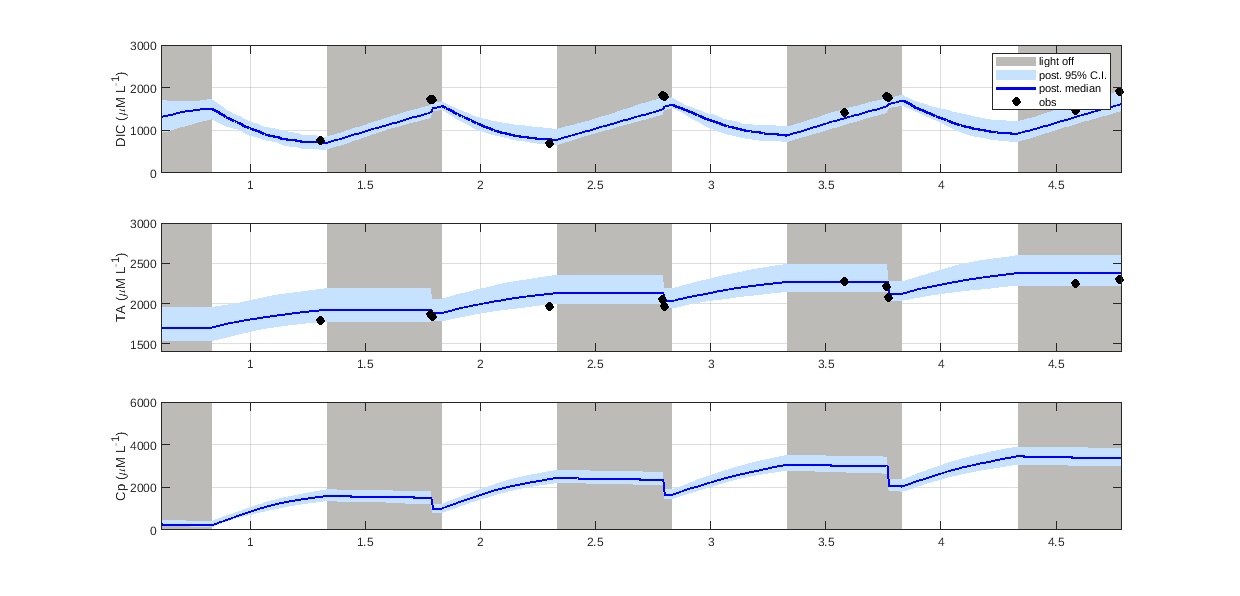
\includegraphics[width=1.2\textwidth]{images_microalgae/plots_chris_offset/DIC_TA_Cp}}
	\caption[.]{Posterior medians (solid blue line), 95\% credible intervals (shaded blue), and observations (black) for $DIC$, $TA$ and $C_p$ across 4 days.}
	\label{fig:micro_exp_offset_DIC_TA_Cp}
\end{figure}

\begin{figure}
	\centerline{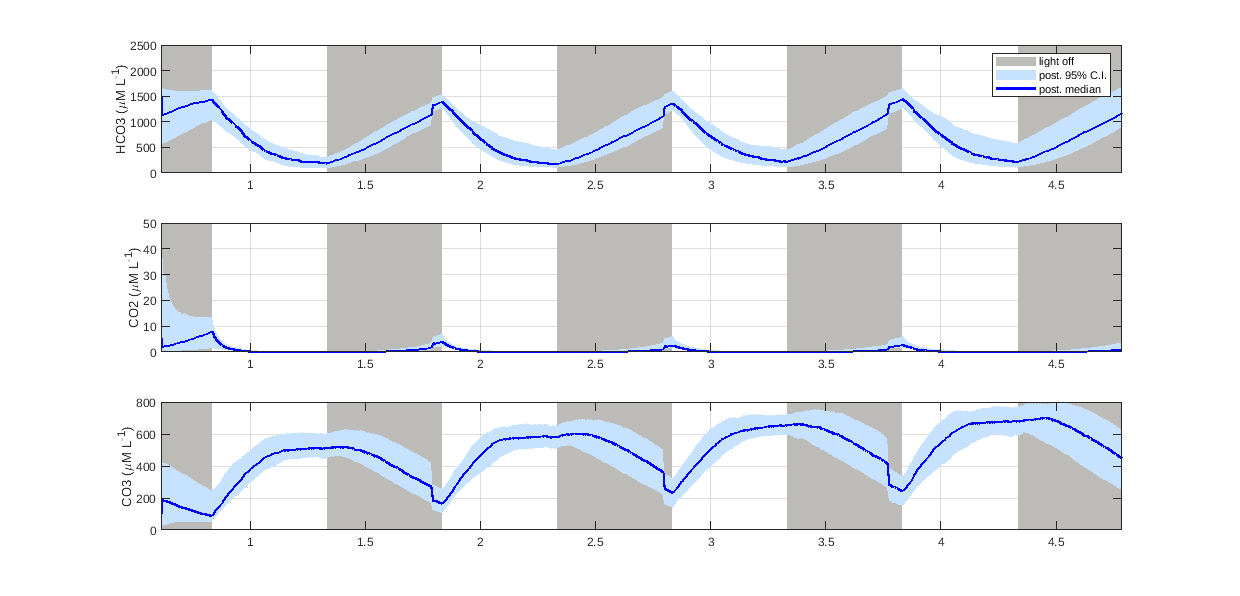
\includegraphics[width=1.2\textwidth]{images_microalgae/plots_chris_offset/carbon}}
	\caption[.]{Posterior medians (solid blue line) and 95\% credible intervals (shaded blue) for $HCO_3$, $CO_2$ and $CO_3$ across 4 days.}
	\label{fig:micro_exp_offset_carbon}
\end{figure}

\begin{figure}
	\centerline{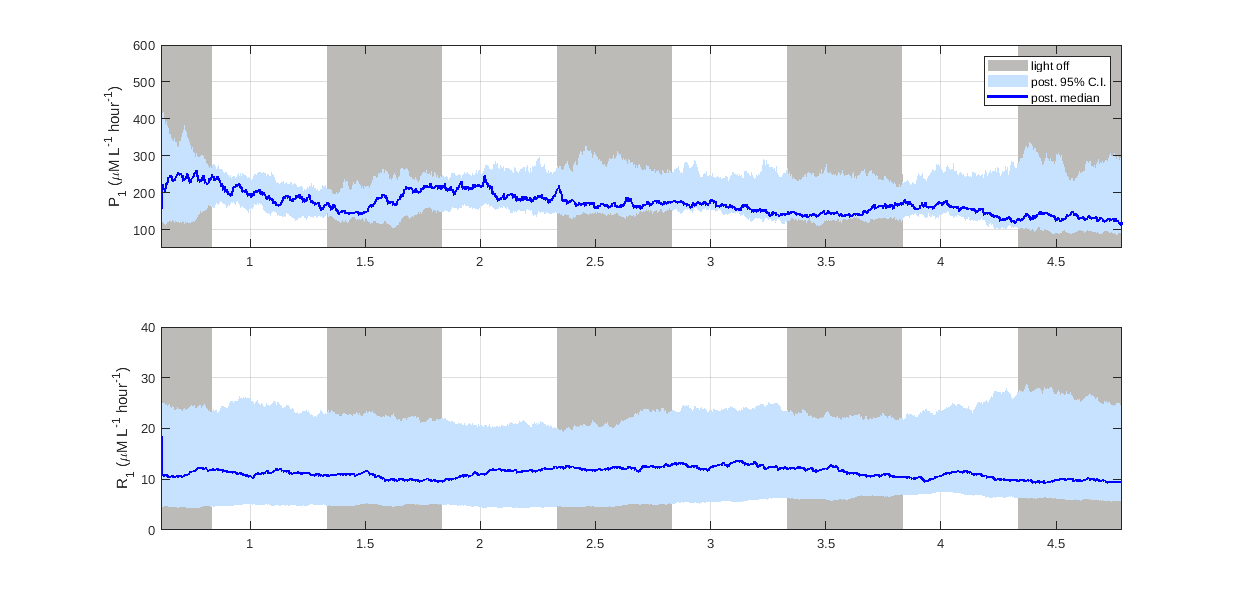
\includegraphics[width=1.2\textwidth]{images_microalgae/plots_chris_offset/P_and_R}}
	\caption[.]{Posterior medians (solid blue line) and 95\% credible intervals (shaded blue) for photosynthesis $P_1$ and respiration $R_1$.}
	\label{fig:micro_exp_offset_P_R}
\end{figure}

\begin{figure}
	\centerline{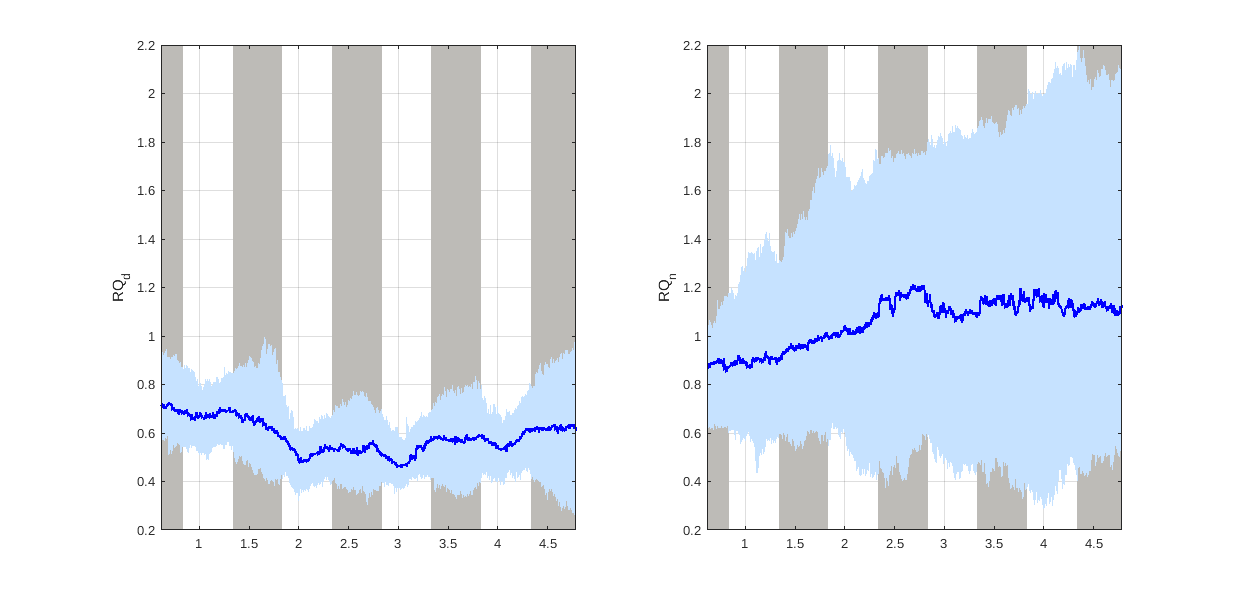
\includegraphics[width=1.2\textwidth]{images_microalgae/plots_chris_offset/RQ_d_RQ_n}}
	\caption[.]{Posterior medians (solid blue line) and 95\% credible intervals (shaded blue) for respiratory quotients $RQ_d$ and $RQ_n$.}
	\label{fig:micro_exp_offset_RQ_d_RQ_n}
\end{figure}



\begin{figure}
	\centerline{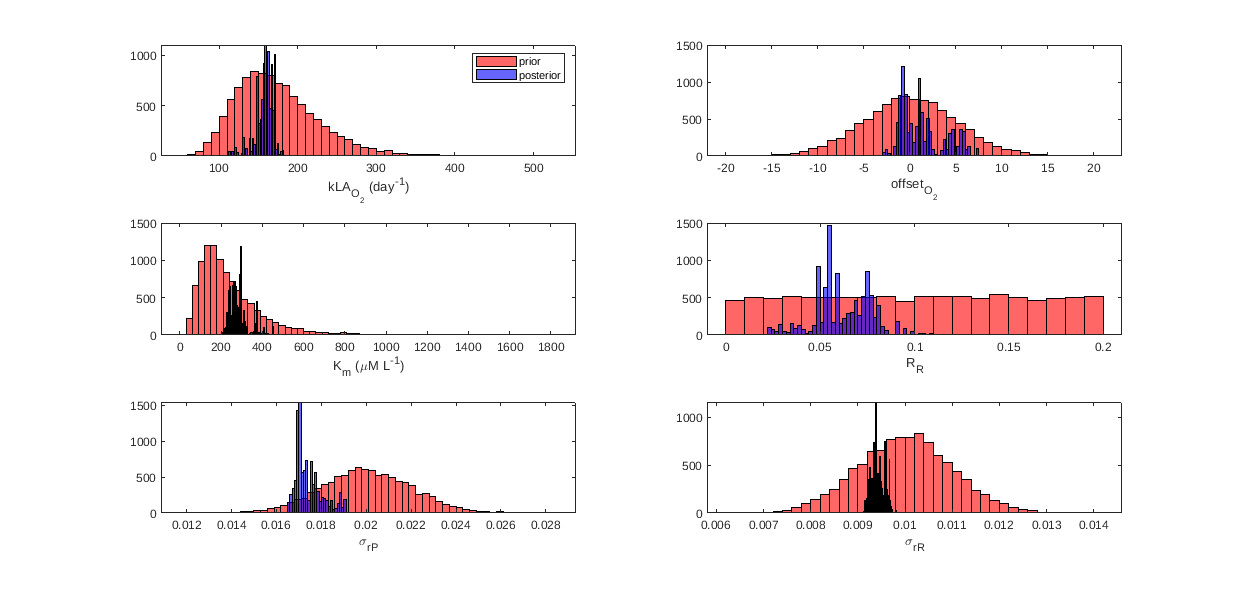
\includegraphics[width=1.3\textwidth]{images_microalgae/plots_chris_offset/modelparameters1}}
	\caption[.]{Priors (pink) and posteriors (purple) for model parameters.}
	\label{fig:micro_exp_offset_parameters_model}
\end{figure}

\begin{figure}
	\centerline{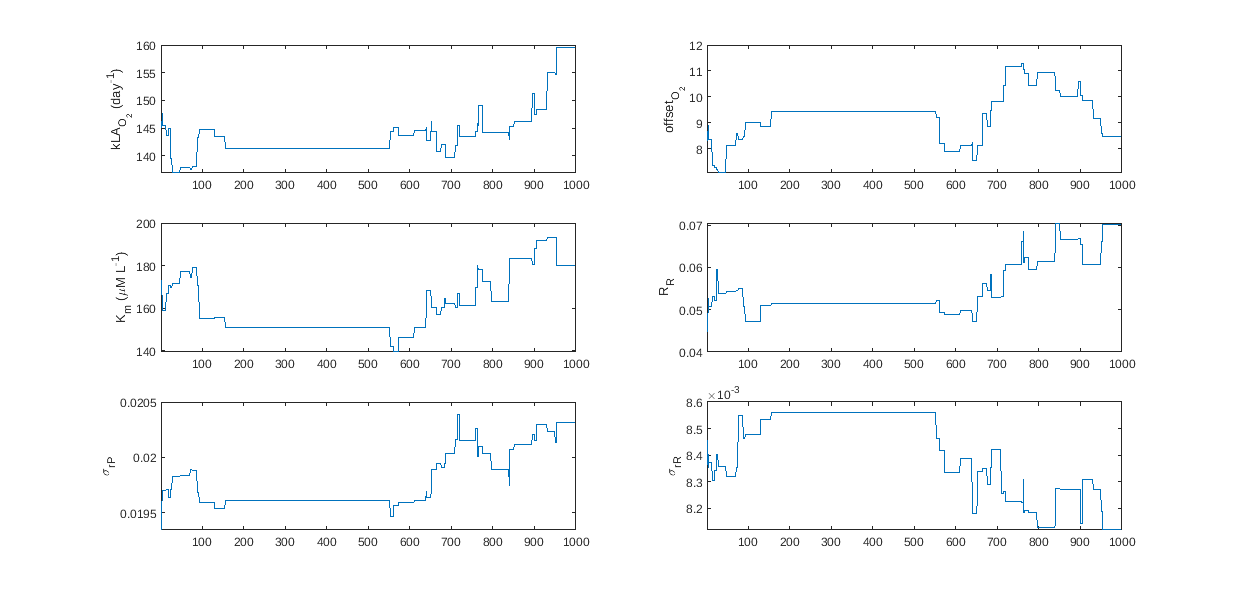
\includegraphics[width=1.3\textwidth]{images_microalgae/plots_chris_offset/modelparameters1_trace}}
	\caption[.]{Model parameter traces.}
	\label{fig:micro_exp_offset_parameters_model_traces}
\end{figure}



\begin{longtable}{|c|c|c|} 
	\hline
	\bfseries{Parameter}  & \bfseries{Quantiles (25\%, 75\%)}  & \bfseries{Quantiles (5\%, 95\%)} \\ \hline
	$kLA_{O_2}^{air}$ 	& (147.0307, 161.6729)  & (139.0878, 171.0318)   \\
	$K_m$ 				& (264.5106, 373.5021) 	& (157.8467, 485.1311) 	 \\ 
	$R_R$ 				& (0.1538, 0.1701) 		& (0.1403, 0.1963) 		 \\
	$\sigma_{r_P}$ 		& (0.0180, 0.0190) 		& (0.0176, 0.0194) 		 \\ 
	$\sigma_{r_R}$ 		& (0.0097, 0.0100) 		& (0.0096, 0.0102)		 \\ 
	$offset_{O_2}$ 		& (0.3097, 2.4730) 	& (-1.2734, 3.5217)		 \\ 	
	\hline
	\caption[.]{Posterior (25\%, 75\%), (5\%, 95\%) quantiles for parameters after assimilating observations.}	
	\label{table:micro_exp_offset_parameters_table}
\end{longtable}

The PMMH was run for 20,000 samples with 2048 particles, where 10,000 samples were discarded as burn-in. 20,000 samples were all that could complete with 2048 particles in the maximum time allocation on the hpc cluster. The number of particles was doubled to test whether this improved mixing, changes to proposal parameters were also trialled.

Observed state variables $DIC$ and $TA$ posteriors perform well with all observations lying within the 95\% credible intervals (Figure \ref{fig:micro_exp_offset_DIC_TA_Cp}). $O_2$ posteriors tracked the observations excellently while the light was on, with all observations falling inside tightly constrained 95\% credible intervals. During times when there was no light, each day the posteriors would fit the observations well to start and then potentially there was a sensor drift causing increasing observations that the model was not accounting for (Figure \ref{fig:micro_exp_offset_O2_pH}). $pH$ captured most observations within the 95\% credible intervals (Figure \ref{fig:micro_exp_offset_O2_pH}).

The photosynthesis rate ($P_1$) was centred between 200 and 250$\mskip3mu$$\mu$M L$^{-1}$ hour$^{-1}$ oscillating subtly with daylight peaks. The 95\% credible intervals lay approximately between 150$\mskip3mu$$\mu$M L$^{-1}$ hour$^{-1}$ and 400$\mskip3mu$$\mu$M L$^{-1}$ hour$^{-1}$ with tighter intervals at the start of each day (Figure \ref{fig:micro_exp_offset_P_R}).
The respiration rate ($R_1$) remained centred around 9$\mskip3mu$$\mu$M L$^{-1}$ hour$^{-1}$ with 95\% credible intervals between 4$\mskip3mu$$\mu$M L$^{-1}$ hour$^{-1}$ and 20$\mskip3mu$$\mu$M L$^{-1}$ hour$^{-1}$ through the course of the experiment (Figure \ref{fig:micro_exp_offset_P_R}).

The day-time respiratory quotient $RQ_d$ was centred around 0.7 with a 95\% credible interval of 0.6-0.9 during the first day of the experiment. The centre dropped to 0.5 during the 2nd, 3rd, and 4th days with tighter 95\% credible intervals of 0.4-0.6 (Figure \ref{fig:micro_exp_offset_RQ_d_RQ_n}). The night-time respiratory quotient $RQ_n$ was initially centred around 0.9 and slowly rose to 1.1 by the second day and continued around 1.1 for the remainder of the experiment. The 95\% credible intervals started with 0.6-1 and increased its span steadily to 0.5-2 by the end of the experiment (Figure \ref{fig:micro_exp_offset_RQ_d_RQ_n}).


Cp
carbon
parameters
first time introduced an offset


Overall, mixing of the PMMH was poor with an acceptance rate of 3.57\% and slowly mixing parameter traces with some correlation between samples that were unable to be improved by increasing particles or tweaking proposal distributions (Figure \ref{fig:micro_exp_offset_parameters_model_traces}). Improving mixing is the focus of the next section (Section \ref{sec:micro_exp_offset_thinned}). 


\FloatBarrier
\subsection{Posterior results with experimental data where photosynthesis, respiration and respiratory quotients are changing through time, $O_2$ has an offset and the $O_2$ observations were thinned further}\label{sec:micro_exp_offset_thinned}
% micro_iterative_chris_offset_thinned.bi


\begin{figure}
	\centerline{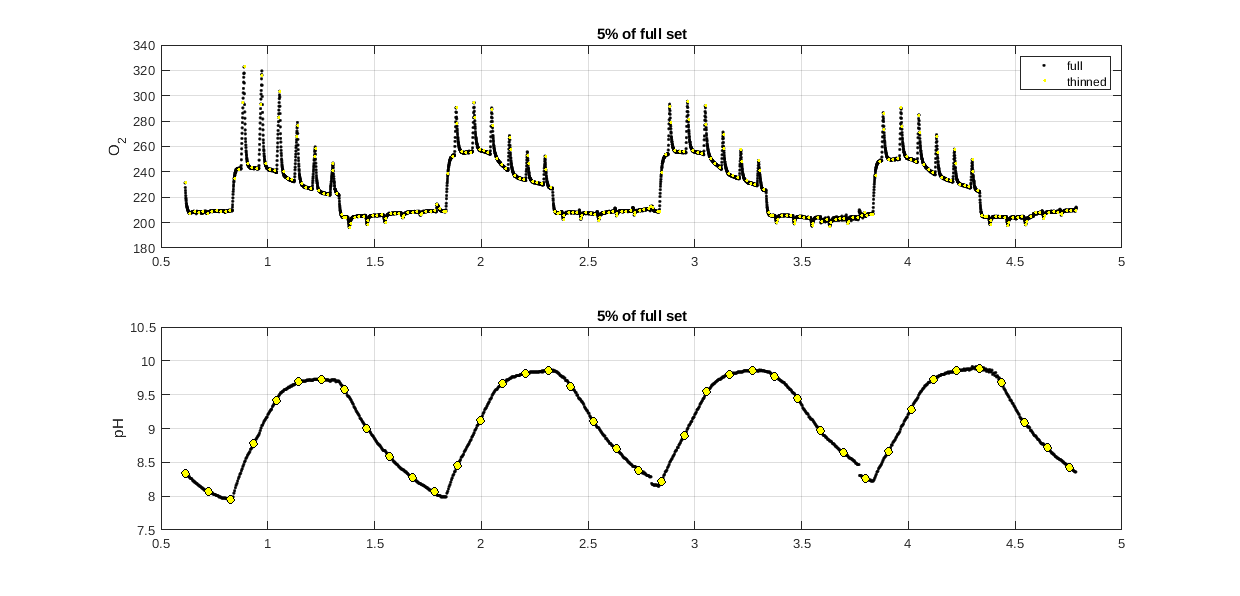
\includegraphics[width=1.25\textwidth]{images_microalgae/plots/thinned_obs_micro_further}}
	\caption[.]{Full $O_2$ and $pH$ datasets with further thinned $O_2$ and $pH$ observations.}
	\label{fig:thinned_obs_further_micro}
\end{figure}

This section aimed to test whether thinning out the $O_2$ observations further (Figure \ref{fig:thinned_obs_further_micro}) helped improve the poorly mixed chain of Section \ref{sec:micro_exp_offset}. All priors and model specifications remained the same as Section \ref{sec:micro_exp_offset}, with the only difference being the further reduced $O_2$ dataset to 5\% of the full observation set.


\begin{figure}
	\centerline{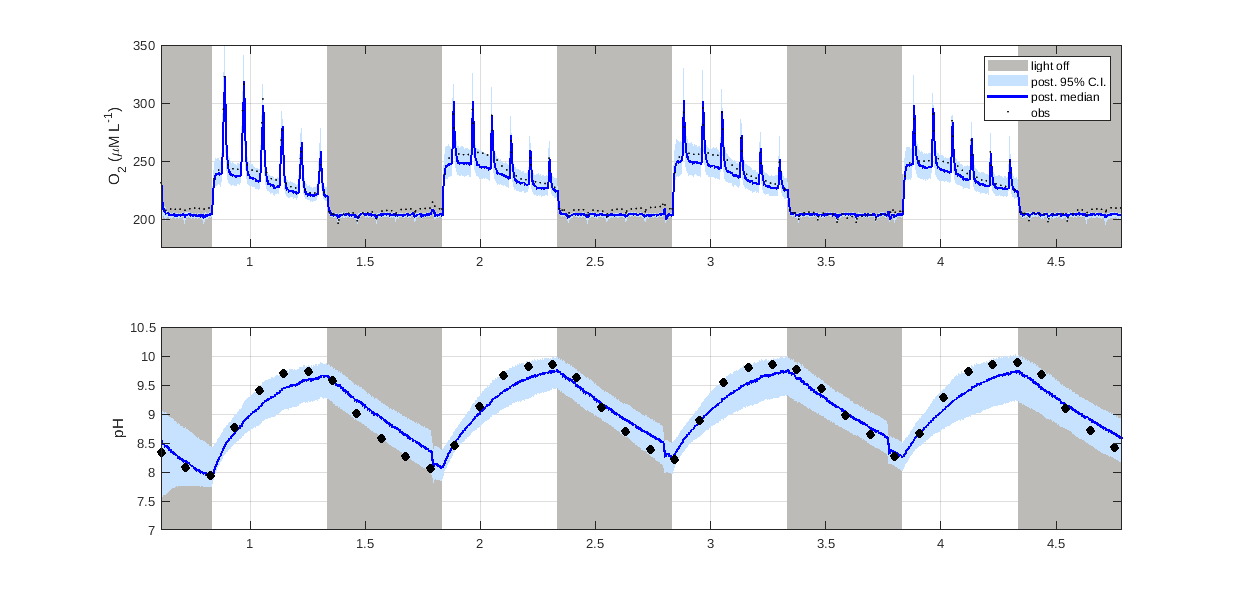
\includegraphics[width=1.2\textwidth]{images_microalgae/plots_chris_offset_thinned/O2_pH}}
	\caption[.]{Posterior medians (solid blue line), 95\% credible intervals (shaded blue), and observations (black) for $O_2$ and $pH$ across 4 days.}
	\label{fig:micro_offset_thinned_O2_pH}
\end{figure}


\begin{figure}
	\centerline{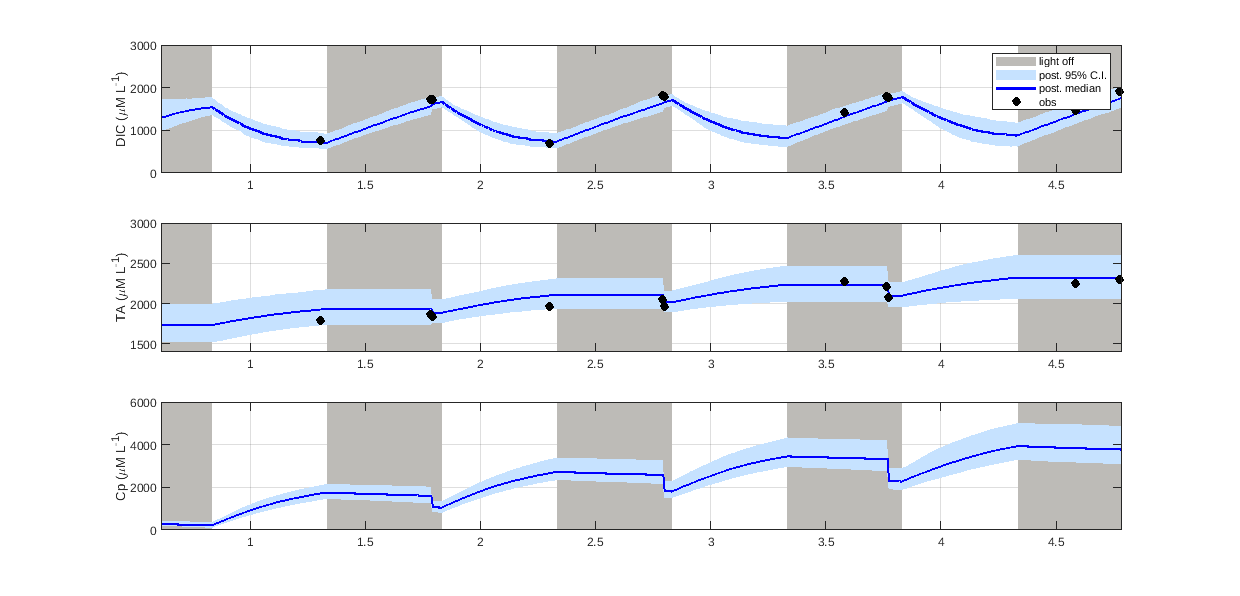
\includegraphics[width=1.2\textwidth]{images_microalgae/plots_chris_offset_thinned/DIC_TA_Cp}}
	\caption[.]{Posterior medians (solid blue line), 95\% credible intervals (shaded blue), and observations (black) for $DIC$, $TA$ and $C_p$ across 4 days.}
	\label{fig:micro_offset_thinned_DIC_TA_Cp}
\end{figure}

\begin{figure}
	\centerline{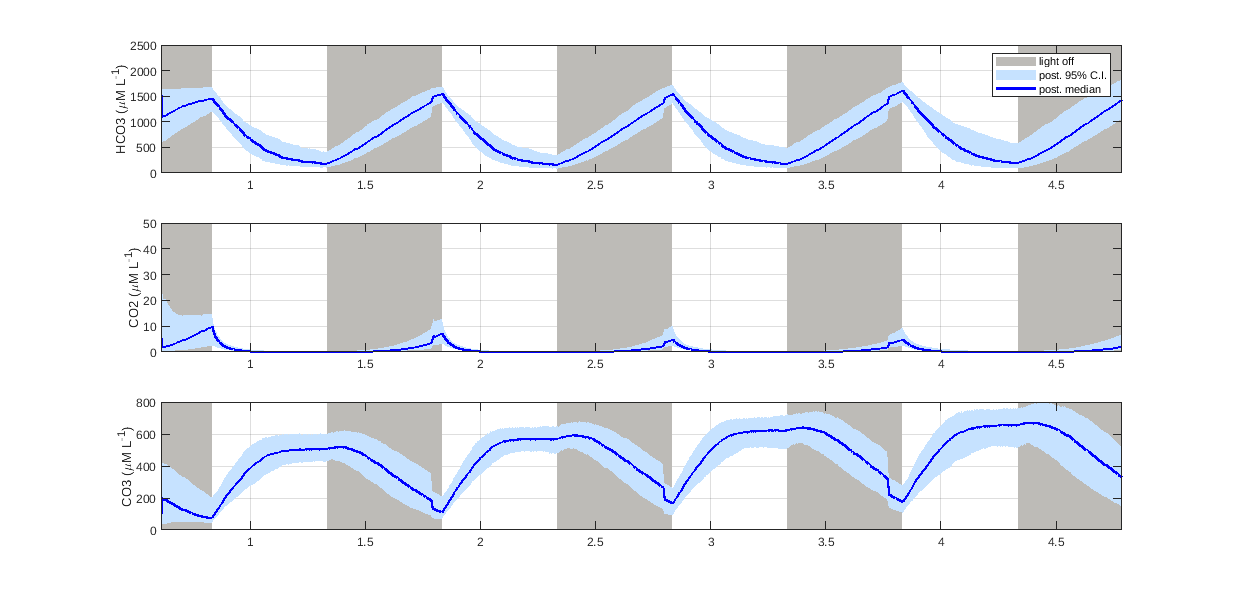
\includegraphics[width=1.2\textwidth]{images_microalgae/plots_chris_offset_thinned/carbon}}
	\caption[.]{Posterior medians (solid blue line) and 95\% credible intervals (shaded blue) for $HCO_3$, $CO_2$ and $CO_3$ across 4 days.}
	\label{fig:micro_offset_thinned_carbon}
\end{figure}

\begin{figure}
	\centerline{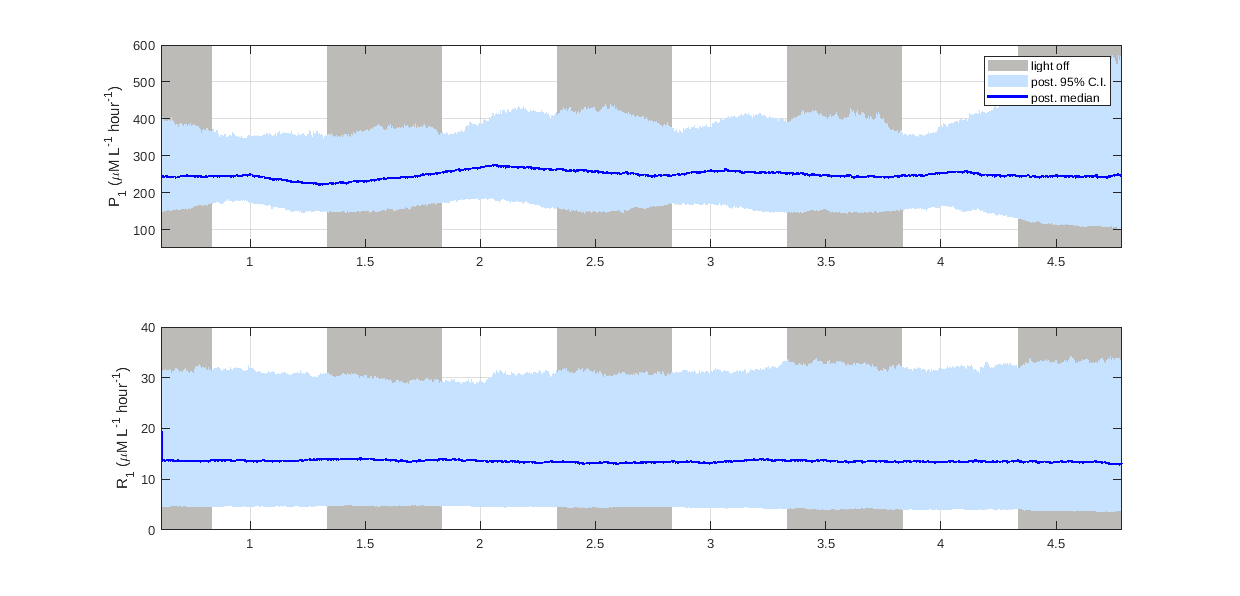
\includegraphics[width=1.2\textwidth]{images_microalgae/plots_chris_offset_thinned/P_and_R}}
	\caption[.]{Posterior medians (solid blue line) and 95\% credible intervals (shaded blue) for photosynthesis $P_1$ and respiration $R_1$.}
	\label{fig:micro_offset_thinned_P_and_R}
\end{figure}

\begin{figure}
	\centerline{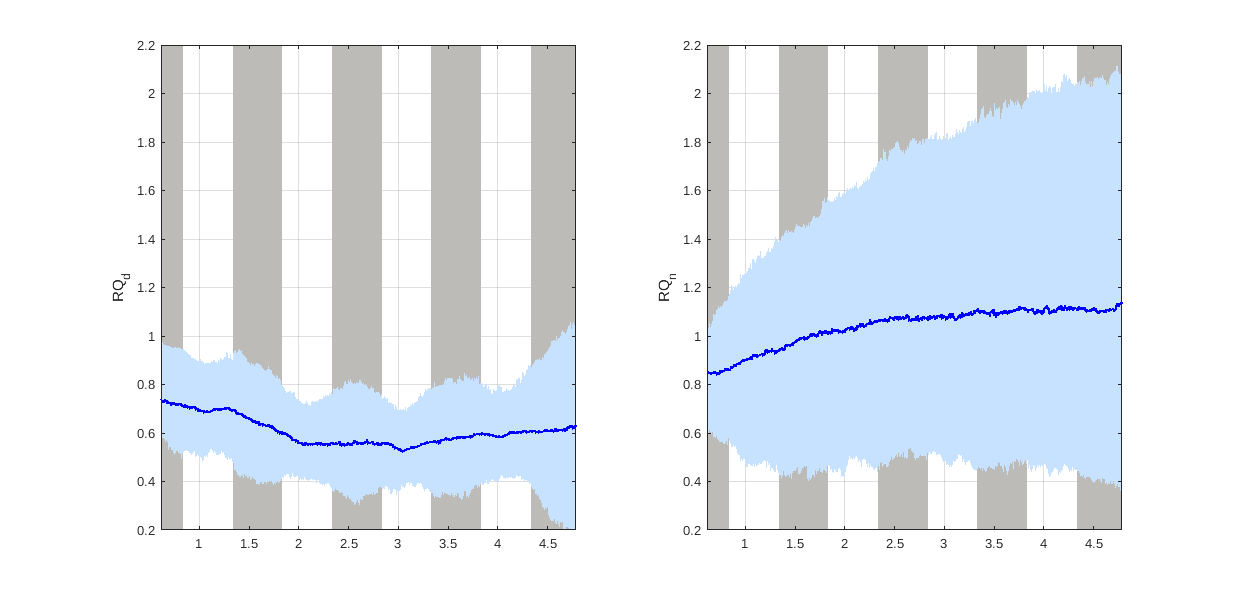
\includegraphics[width=1.2\textwidth]{images_microalgae/plots_chris_offset_thinned/RQ_d_RQ_n}}
	\caption[.]{Posterior medians (solid blue line) and 95\% credible intervals (shaded blue) for respiratory quotients $RQ_d$ and $RQ_n$.}
	\label{fig:micro_offset_thinned_RQ_d_RQ_n}
\end{figure}

\begin{figure}
	\centerline{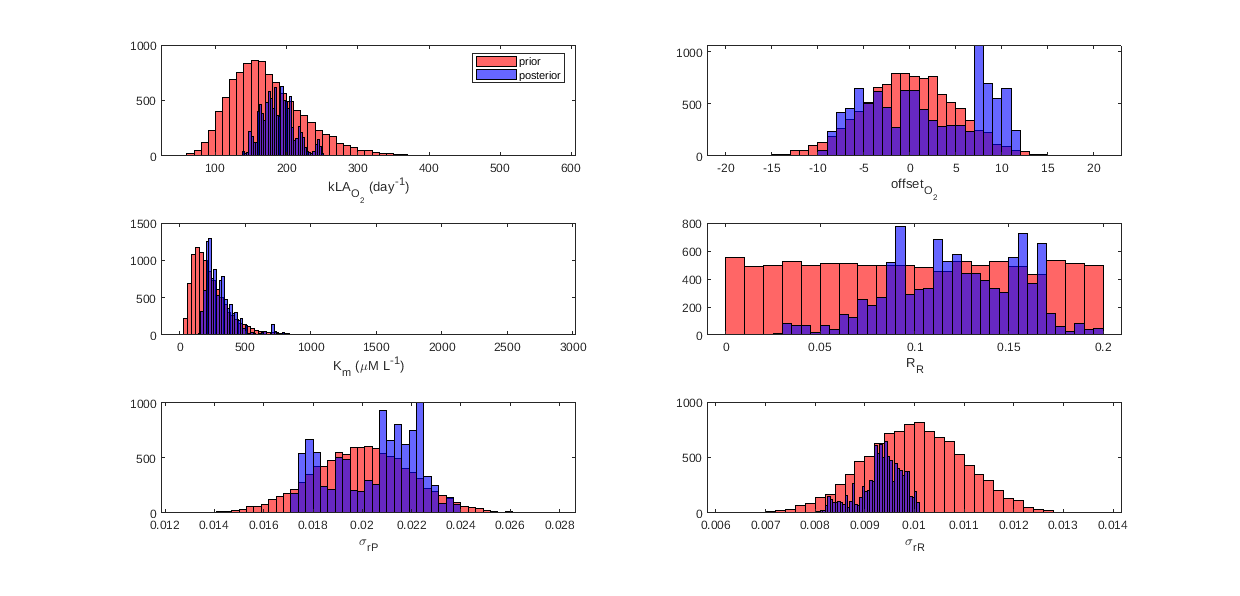
\includegraphics[width=1.3\textwidth]{images_microalgae/plots_chris_offset_thinned/modelparameters1}}
	\caption[.]{Priors (pink) and posteriors (purple) for model parameters.}
	\label{fig:micro_offset_thinned_parameters_model}
\end{figure}

\begin{figure}
	\centerline{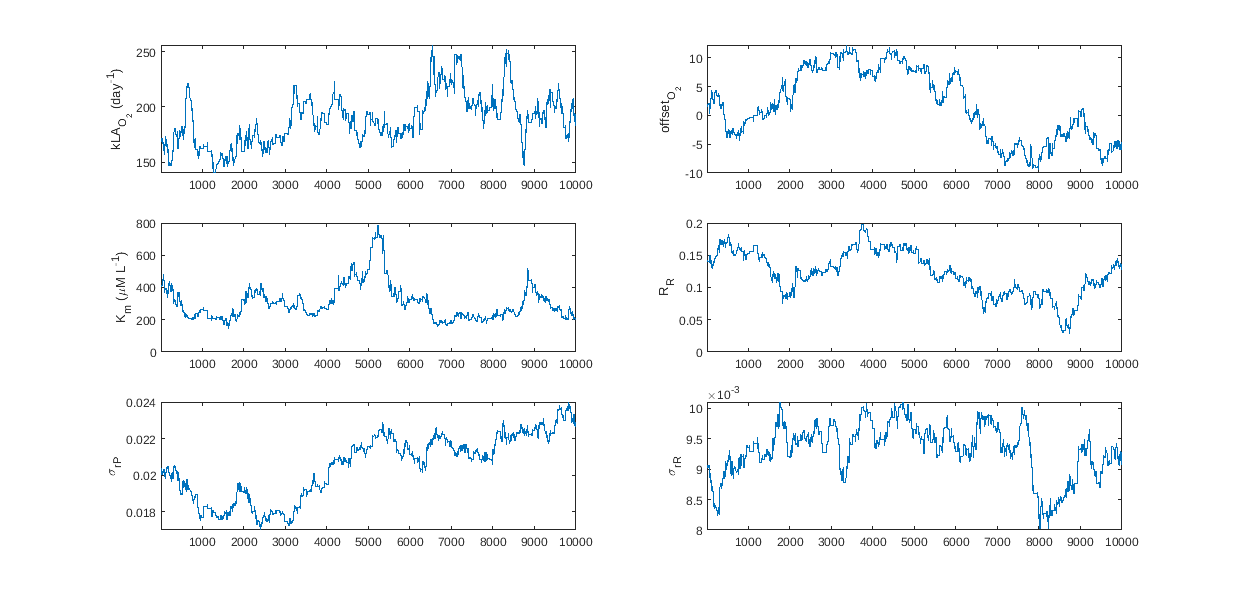
\includegraphics[width=1.3\textwidth]{images_microalgae/plots_chris_offset_thinned/modelparameters1_trace}}
	\caption[.]{Model parameter traces.}
	\label{fig:micro_offset_thinned_parameters_model_trace}
\end{figure}


\begin{longtable}{|c|c|c|} 
	\hline
	\bfseries{Parameter}  & \bfseries{Quantiles (25\%, 75\%)}  & \bfseries{Quantiles (5\%, 95\%)} \\ \hline
	$kLA_{O_2}^{air}$ 	& (172.4048, 202.2482)  & (153.4338, 227.8861)   \\
	$K_m$ 				& (224.2554, 352.8140) 	& (183.9269, 506.7944) 	 \\ 
	$R_R$ 				& (0.0939, 0.1527) 		& (0.0639, 0.1684) 		 \\
	$\sigma_{r_P}$ 		& (0.0190, 0.0220) 		& (0.0176, 0.0229) 		 \\ 
	$\sigma_{r_R}$ 		& (0.0091, 0.0096) 		& (0.0084, 0.0099)		 \\ 
	$offset_{O_2}$ 		& (-3.6927, 7.7906) 	& (-7.4953, 10.7980)		 \\ 	
	\hline
	\caption[.]{Posterior (25\%, 75\%), (5\%, 95\%) quantiles for parameters after assimilating observations.}	
	\label{table:micro_exp_offset_thinned_parameters_table}
\end{longtable}

Similarly to Section \ref{sec:micro_exp_offset}, 20,000 samples were run (10,000 discarded as burn-in) with 2048 particles. The acceptance rate improved to 13.61\% with less dense observations. 

There was an improvement in $pH$ posterior with the 95\% credible interval now capturing all observations (Figure \ref{fig:micro_offset_thinned_O2_pH}).
Visually there does not appear to be much difference in $O_2$ posterior with both runs capturing the same observations within their 95\% credible intervals. The credible intervals are wider during the day for the further thinned observations when compared to Figure \ref{fig:micro_exp_offset_O2_pH}.
There was not much difference between posteriors for $DIC$, $TA$, and $C_p$ (Figure \ref{fig:micro_offset_thinned_DIC_TA_Cp}) apart from the $C_p$ 95\% credible interval being wider when there are less $O_2$ observations.
Similarly, the carbon chemistry behaved similarly in both sections (Figure \ref{fig:micro_offset_thinned_carbon}).

$P_1$ behaved similarly across sections, with more smoothness through the median and slightly wider credible intervals when less $O_2$ observations were assimilated. $R_1$ notably was centred around 15$\mskip3mu$$\mu$M L$^{-1}$ hour$^{-1}$ with 95\% credible intervals 5-30$\mskip3mu$$\mu$M L$^{-1}$ hour$^{-1}$ (Figure \ref{fig:micro_offset_thinned_P_and_R}) compared to 9$\mskip3mu$$\mu$M L$^{-1}$ hour$^{-1}$ with 95\% credible intervals between 4$\mskip3mu$$\mu$M L$^{-1}$ hour$^{-1}$ and 20$\mskip3mu$$\mu$M L$^{-1}$ hour$^{-1}$ (Figure \ref{fig:micro_exp_offset_P_R}). 
Respiratory quotients had smoother medians throughout the experiment with less $O_2$ data (Figure \ref{fig:micro_offset_thinned_RQ_d_RQ_n}) otherwise not much change. 


$kLA_{O_2}^{air}$ posterior shifted to higher values compared to Section \ref{sec:micro_exp_offset}. $offset_{O_2}$ had a wider posterior than that of the previous section but still centred around approximately the same value.
$K_m$ posterior shifted to lower values while $R_R$ displayed a wider posterior distribution than the previous section while being centred lower.
Posteriors for $\sigma_{rP}$ and $\sigma_{rR}$ were both wider when there were less $O_2$ observations to be assimilated (Figure \ref{fig:micro_offset_thinned_parameters_model}).
Parameter traces improved their mixing (Figure \ref{fig:micro_offset_thinned_parameters_model_trace}) from Section \ref{sec:micro_exp_offset}, but still displayed correlation between samples.



\FloatBarrier
\section{Discussion}

Learnings by result section:



After thinning out the $O_2$ observations further, the acceptance rate and mixing improved in Section \ref{sec:micro_exp_offset_thinned} but still was not ideal. Correlated samples were present.
Apart from smoothing  out some of the state variable posteriors, and subtly wider 95\% credible intervals, there was not much difference in posterior results between Section \ref{sec:micro_exp_offset} and Section \ref{sec:micro_exp_offset_thinned} where the $O_2$ observations were thinned further





Non destructive measurements allow us to use sensors to obtain these measurements instead of destructive sampling techniques. Meaning we can get informative estimates from well calibrated sensor measurements that combined with a data assimilating model can 



Model states are sensitive to small perturbations in parameters. This is why instrument calibration for measurements is essential. [BM: maybe show a python run with different values of temp, constants etc to show the sensitivity? Or maybe just talk about it.] 


Possibilities for RQn going well outside what the biology would allow. 
More processes taking place than what we currently have in the model description. We have a parameter $RQ_n$ that can compensate for the input $O_2$ gas line may have dropped or increased.
In the model $O_2$ concentration is treated as fixed when in reality this is an unmodelled process. If it's taking air in during the night time in the lab, it might go higher because there are less people there 
diurnal changes a possibility also, therefore can go up can go down.
Henry's law shift 
future work: can measure this too.

when you constrain those two to be between 0.6 and 1, we see things like in the other runs where they slam up against the edge values of the priors and the sampling and mixing goes to shit.

sigma starts going to 0, for estimating the obs error.

bias in instrument errors in completely unmeasured, where the noise on the instrument error is easily measurable, bias on the other hand is not.

Big achievement for this chapter: putting the CO2SYS stuff (if you don't get CO2SYS right then you start getting all sorts of crazy values like negative values etc. CO2SYS is especially sensistive because CO2 is whats controlling the fluxes , must be accurate, HCO3 is in the thousands so the errors need to be tiny because we have huge numbers for HCO3 and tiny numbers for CO2 need to be tiny, need to be really accurate. then pH which is on a log scale means that making a mistake at one part is completely different to making a mistake at another part.) into libbi which opens it up to details and nonlinear processes. getting this to work in the libbi constraints which are using gpus and very simple statistical models- letting us expand this in the mathematical sense for more complex models and equations. this would be the same limitation as stan on the gpu complexitity of model side of things.


Discuss increasing the number of particles and changing the proposal distribution but how this had little effect on the mixing. Discuss mixing and correlation overall in reference to each results section.

Unbalanced weights of observations- $O_2$ and $pH$ have much denser datasets than $DIC$ and $TA$. When these densely populated datasets are too frequent, this causes problems in the likelihood estimation 
[This issue of how to combine  fuse different measurements with huge differences in sampling density is an interesting one]

Discuss failed experiments and why. Maybe add them to the appendix and reference them here.


% Calculate DIC for each model that had the same set of obs to compare which one performs better.



\appendix

\chapter{LiBbi model code}\label{appendix_micro_libbi_code}

\textbf{LiBbi model file: micro\_iterative.bi}
\begin{lstlisting}
model micro_iterative {

const FO2	= 0.2094
const FCO2	= 397e-6
const S		= 34.0
const V		= 500.0			// volume of the reactor
const DIC_M	= 1724.20		// calculated with CO2SYS[DIC_M = 1724.20, Alk = 1797.90, T = 27, S = 34]
const O_2_M	= 226.65
const alk_M	= 1797.90
const tau	= 6.0
const kLAO2_m	= log(2.0)*24.0*60.0/tau

param kLAO2
param Km
param RR
param RQ_d
param RQ_n
param sigma_O_2
param sigma_pH
param sigma_DIC
param offset_O_2

input I			// light intensity
input T			// temperature (C)
input gas		// gas on/off
input dil		// dilution rate

state DIC // state variables
state O_2
state pH
state Cp
state mich_ment
state O2H_pr
state CO2H_pr
state R
state R1
state P
state P1
state alk
state CO2
state HCO3
state CO3
state O_2H
state CO2H
state h_3
state h_free_3

noise r_R
noise r_P

/* random walk parameter */
param sigma_r_R
param sigma_r_P

obs O2_obs
obs pH_obs
obs DIC_obs
obs alk_obs

sub parameter {/* prior distribution over parameters */
Km 	~ log_normal(log(100.0), 0.5)
kLAO2 	~ log_normal(log(kLAO2_m), 0.3)
RR 	~ uniform(0.0001, 0.2)
RQ_d	~ uniform(0.66, 1.0)
RQ_n	~ uniform(0.66, 1.0)

sigma_O_2 ~ log_normal(log(0.03), 0.5)
sigma_pH  ~ log_normal(log(0.03), 0.5)
sigma_DIC ~ log_normal(log(0.03), 0.5)

offset_O_2 ~ normal(0, 2.0)

sigma_r_R 	~ normal(0.01, 0.001)
sigma_r_P 	~ normal(0.05, 0.01)
}

const prop_std = 0.1;
sub proposal_parameter {
Km 	~ log_normal(log(Km), 0.5*prop_std)
kLAO2 	~ log_normal(log(kLAO2), 0.3*prop_std)
RR 	~ truncated_normal(RR, 0.2*prop_std, lower = 0.0001, upper = 0.2)
RQ_d 	~ truncated_normal(RQ_d, 0.2*prop_std, lower = 0.66, upper = 1.0)
RQ_n 	~ truncated_normal(RQ_n, 0.2*prop_std, lower = 0.66, upper = 1.0)


sigma_O_2 	~ log_normal(log(sigma_O_2), 0.5*prop_std)
sigma_pH 	~ log_normal(log(sigma_pH), 0.5*prop_std)
sigma_DIC 	~ log_normal(log(sigma_DIC), 0.5*prop_std)

offset_O_2	~ normal(offset_O_2, 2.0*prop_std)

sigma_r_R 	~ normal(sigma_r_R, 0.001*prop_std)
sigma_r_P 	~ normal(sigma_r_P, 0.01*prop_std)
}

sub initial {/* prior distribution over initial conditions, given parameters */
// specify the initial condition model 
R 	~ normal(log(20.0), 0.4)
R1 	~ log_normal(log(20.0), 0.4)
P 	~ normal(log(200.0), 0.4)
P1 	~ log_normal(log(200.0), 0.4)

Cp	~ log_normal(log(300.0), 0.2)	
alk 	~ log_normal(log(1750.0), 0.1)
DIC 	~ log_normal(log(1300.0), 0.2) 
O_2 	~ log_normal(log(225.0), 0.2)   
pH 	~ log_normal(log(8.5), 0.2)
CO2 	~ log_normal(log(3.0), 0.4)
HCO3 	~ log_normal(log(1000.0), 0.3)
CO3 	~ log_normal(log(300.0), 0.4)
O_2H 	~ log_normal(log(200.0), 0.2)	
CO2H 	~ log_normal(log(10.0), 0.2)
}


//sub transition(delta = 0.0023) { // obs are in days ie delta=1.0 for daily solving. delta=0.00069 for solving every minute, 0.0014 for every 2 mins, 0.0021 for 3 mins, 0.0028 for 4mins, delta=0.000011574 for solving every second
sub transition(delta = 0.0021) { 

/* processes */

inline TK     = T + 273.15		// temp in kelvin
inline K0_CO2 = exp(-60.2409 + 93.4517*(100.0/TK) + 23.3585*log(TK/100.0)+ S*(0.023517 - 0.023656*(TK/100) + 0.0047036*(TK/100.0)*(TK/100.0)))
CO2H          <- K0_CO2*FCO2*1.0220*1e6

inline K0_O2  =  (exp(-1282.8704 + 36619.96/TK + 223.1396*log(TK) -0.354707*TK + S*(5.957e-3 -3.7353/TK) + 3.68e-6*S*S))/(0.2094e-06)
O_2H 	      <- K0_O2*FO2*1.0220*1e-6

inline PAC    = HCO3  		//PAC=photosynthetically active carbon. if the phyto are just using CO2 to photosynthesise then PAC=CO2
inline mm     = PAC/(Km + PAC)

// CO2SYS iterative solution
// set up all the constants

inline logTK  = log(TK)
inline S2     = S*S
inline sqrtS  = sqrt(S)

// total sulphur

inline TS     = (0.14/96.062)*(S/1.80655)
inline IS     = 19.924*S/(1000.0 - 1.005*S)

inline KS_int = -4276.1/TK + 141.328 - 23.093*logTK + (-13856.0/TK + 324.57  -  47.986*logTK)*sqrt(IS) + ( 35474.0/TK - 771.54  + 114.723*logTK)*IS - 2698.0/TK*IS**1.5 + 1776.0/TK*IS**2
inline KS     = exp(KS_int)*(1 - 0.001005*S)

// Fluorine

inline TF       = 0.000067*S/18.9984/1.80655
inline KF       = exp(-(-874.0/TK - 0.111*sqrtS + 9.68))
inline SWS_2_T  = (1.0 + TS/KS)/(1.0 + TS/KS + TF/KF)
inline Free_2_T = 1.0 + TS/KS

// H2O dissoc

inline KW = exp(148.9802 - 13847.26/TK  - 23.6521*logTK + (118.67/TK - 5.977 + 1.0495*logTK)*sqrtS - 0.01615*S)

// Boron

inline KB = exp((-8966.90 - 2890.53*sqrtS - 77.942*S + 1.728*S*sqrtS - 0.0996*S2)/TK + 148.0248 + 137.1942*sqrtS + 1.62142*S - (24.4344 + 25.085*sqrtS + 0.2474*S)*logTK + 0.053105*sqrtS*TK)
inline TB = 0.0004326*S/35.0

// Carbon eq constants

inline K1 = 10**(-(3633.86/TK - 61.2172 + 9.6777 *logTK - 0.011555*S + 0.0001152*S**2))*1.23	//1.23 experiment specific and measured 
inline K2 = 10**(-( 471.8/TK + 25.9290 - 3.16967*logTK - 0.01781*S + 0.0001122*S**2))*0.53	//0.53 experiment specific and measured

// end all the constants

// intial guess at the pH (use the approximating equation)

inline pH_init = 12.26 -0.0030605*DIC -0.043752*T -0.013625*S+ 0.00011315*alk + 1.3463e-05*DIC*T + 5.2215e-07*DIC*alk

// iteration 1

inline h_1 	= 10.0**(-pH_init)
inline h_free_1	= h_1/Free_2_T
inline f0_1 	= (DIC*1e-6*(K1*h_1 + 2.0*K1*K2)/(h_1*h_1 + K1*h_1 + K1*K2) - h_free_1 + KW/h_1 - alk*1e-6 + TB/(1.0 + h_1/KB))*1e6
inline df0_1 	= (DIC*1e-6*(K1 + 2.0*K1*K2)/(h_1**2.0 + K1*h_1 + K1*K2) - DIC*1e-6*(K1*h_1 + 2.0*K1*K2)/(h_1**2.0 + K1*h_1 + K1*K2)**2.0*(2.0*h_1 + K1) - TB*1.0/(1.0 + h_1/KB)**2.0/KB - KW/h_1**2.0 - 1.0/Free_2_T)*1e6*(-log(10.0)*10.0**(-pH_init))
inline pH_1	= pH_init - f0_1/df0_1

// iteration 2

inline h_2 	= 10.0**(-pH_1)
inline h_free_2	= h_2/Free_2_T
inline f0_2 	= (DIC*1e-6*(K1*h_2 + 2.0*K1*K2)/(h_2*h_2 + K1*h_2 + K1*K2) - h_free_2 + KW/h_2 - alk*1e-6 + TB/(1.0 + h_2/KB))*1e6
inline df0_2 	= (DIC*1e-6*(K1 + 2.0*K1*K2)/(h_2**2.0 + K1*h_2 + K1*K2) - DIC*1e-6*(K1*h_2 + 2.0*K1*K2)/(h_2**2.0 + K1*h_2 + K1*K2)**2.0*(2.0*h_2 + K1) - TB*1.0/(1.0 + h_2/KB)**2.0/KB - KW/h_2**2.0 - 1.0/Free_2_T)*1e6*(-log(10.0)*10.0**(-pH_1))
inline pH_2 	= pH_1 - f0_2/df0_2  

// iteration 3

h_3 		<- 10.0**(-pH_2)
h_free_3	<- h_3/Free_2_T
inline f0_3  	= (DIC*1e-6*(K1*h_3 + 2.0*K1*K2)/(h_3*h_3 + K1*h_3 + K1*K2) - h_free_3 + KW/h_3 - alk*1e-6 + TB/(1.0 + h_3/KB))*1e6
inline df0_3 	= (DIC*1e-6*(K1 + 2.0*K1*K2)/(h_3**2.0 + K1*h_3 + K1*K2) - DIC*1e-6*(K1*h_3 + 2.0*K1*K2)/(h_3**2.0 + K1*h_3 + K1*K2)**2.0*(2.0*h_3 + K1) - TB*1.0/(1.0 + h_3/KB)**2.0/KB - KW/h_3**2.0 - 1.0/Free_2_T)*1e6*(-log(10.0)*10.0**(-pH_2))
pH 		<- pH_2 - f0_3/df0_3  

// iteration 4

//    	inline h_4 	= 10.0**(-pH_3)
//    	inline h_free_4 = h_4/Free_2_T
//	inline f0_4 	= (DIC*1e-6*(K1*h_4 + 2.0*K1*K2)/(h_4*h_4 + K1*h_4 + K1*K2) - h_free_4 + KW/h_4 - alk*1e-6 + TB/(1.0 + h_4/KB))*1e6
//    	inline df0_4 	= (DIC*1e-6*(K1 + 2.0*K1*K2)/(h_4**2.0 + K1*h_4 + K1*K2) - DIC*1e-6*(K1*h_4 + 2.0*K1*K2)/(h_4**2.0 + K1*h_4 + K1*K2)**2.0*(2.0*h_4 + K1) - TB*1.0/(1.0 + h_4/KB)**2.0/KB - KW/h_4**2.0 - 1.0/Free_2_T)*1e6*(-log(10.0)*10.0**(-pH_3))
//	inline pH_4 	= pH_3 - f0_4/df0_4

//	pH		<- pH_4

// calculate the final concentrations

inline H 	= 10.0**(-pH)
inline H2 	= H*H
inline denom 	= (H2 + K1*H + K1*K2)
CO2  		<- DIC*H2/denom
HCO3 		<- DIC*H*K1/denom
CO3  		<- DIC*K1*K2/denom  

// end CO2SYS iterative solution


/* R and P as random walks */

r_R 	~ normal(0.0, sigma_r_R)
R 	<- R + r_R
R1 	<- exp(R)

r_P ~ normal(0.0, sigma_r_P)
P 	<- P + r_P
P1 	<- exp(P)

ode(h = 0.1, atoler = 1.0e-6, rtoler = 1.0e-6, alg = 'RK4(3)'){
dDIC/dt  =  -P1*24.0*I*mm + R1*24.0 				+ gas*0.893*kLAO2*(CO2H - CO2)		+ dil/V*(DIC_M - DIC)  		 
dO_2/dt	 =  (P1*24.0*I*mm - R1*24.0)/(RQ_d*I + RQ_n*(1.0-I)) 	+ gas*kLAO2*(O_2H - O_2)		+ dil/V*(O_2_M - O_2)	+ offset_O_2 		
dalk/dt  =   RR*P1*24.0*I*mm										+ dil/V*(alk_M - alk)
dCp/dt	 =   (P1*24.0*I*mm - R1*24.0) 									+ dil/V*(Cp)

}

mich_ment <- mm
O2H_pr 	  <- O_2H
CO2H_pr   <- CO2H

}


sub observation {

O2_obs  ~ log_normal(log(O_2), sigma_O_2)
pH_obs  ~ log_normal(log(pH),  sigma_pH)
DIC_obs ~ log_normal(log(DIC), sigma_DIC) 
alk_obs ~ log_normal(log(alk), sigma_DIC)
}
}
\end{lstlisting}

\textbf{LiBbi prior sampling file: prior.conf}
\begin{lstlisting}
--target prior
--model-file micro_iterative.bi
--nsamples 500
--start-time 0.61304
--end-time 4.7866
--noutputs 6049
--input-file data/input_all_2018_normalised.nc
--output-file results/prior_micro_iterative.nc
\end{lstlisting}

\textbf{LiBbi posterior sampling file: posterior.conf}
\begin{lstlisting}
--target posterior
--model-file micro_iterative.bi
--input-file data/input_all_2018_normalised.nc
--obs-file data/obs_all_2018.nc
--nsamples 500
--nparticles 1024
--start-time 0.61304
--end-time 4.7866
--noutputs 6049
--output-file results/posterior_micro_iterative.nc
--with-transform-initial-to-param
\end{lstlisting}

\begin{sidewaysfigure}
	\centerline{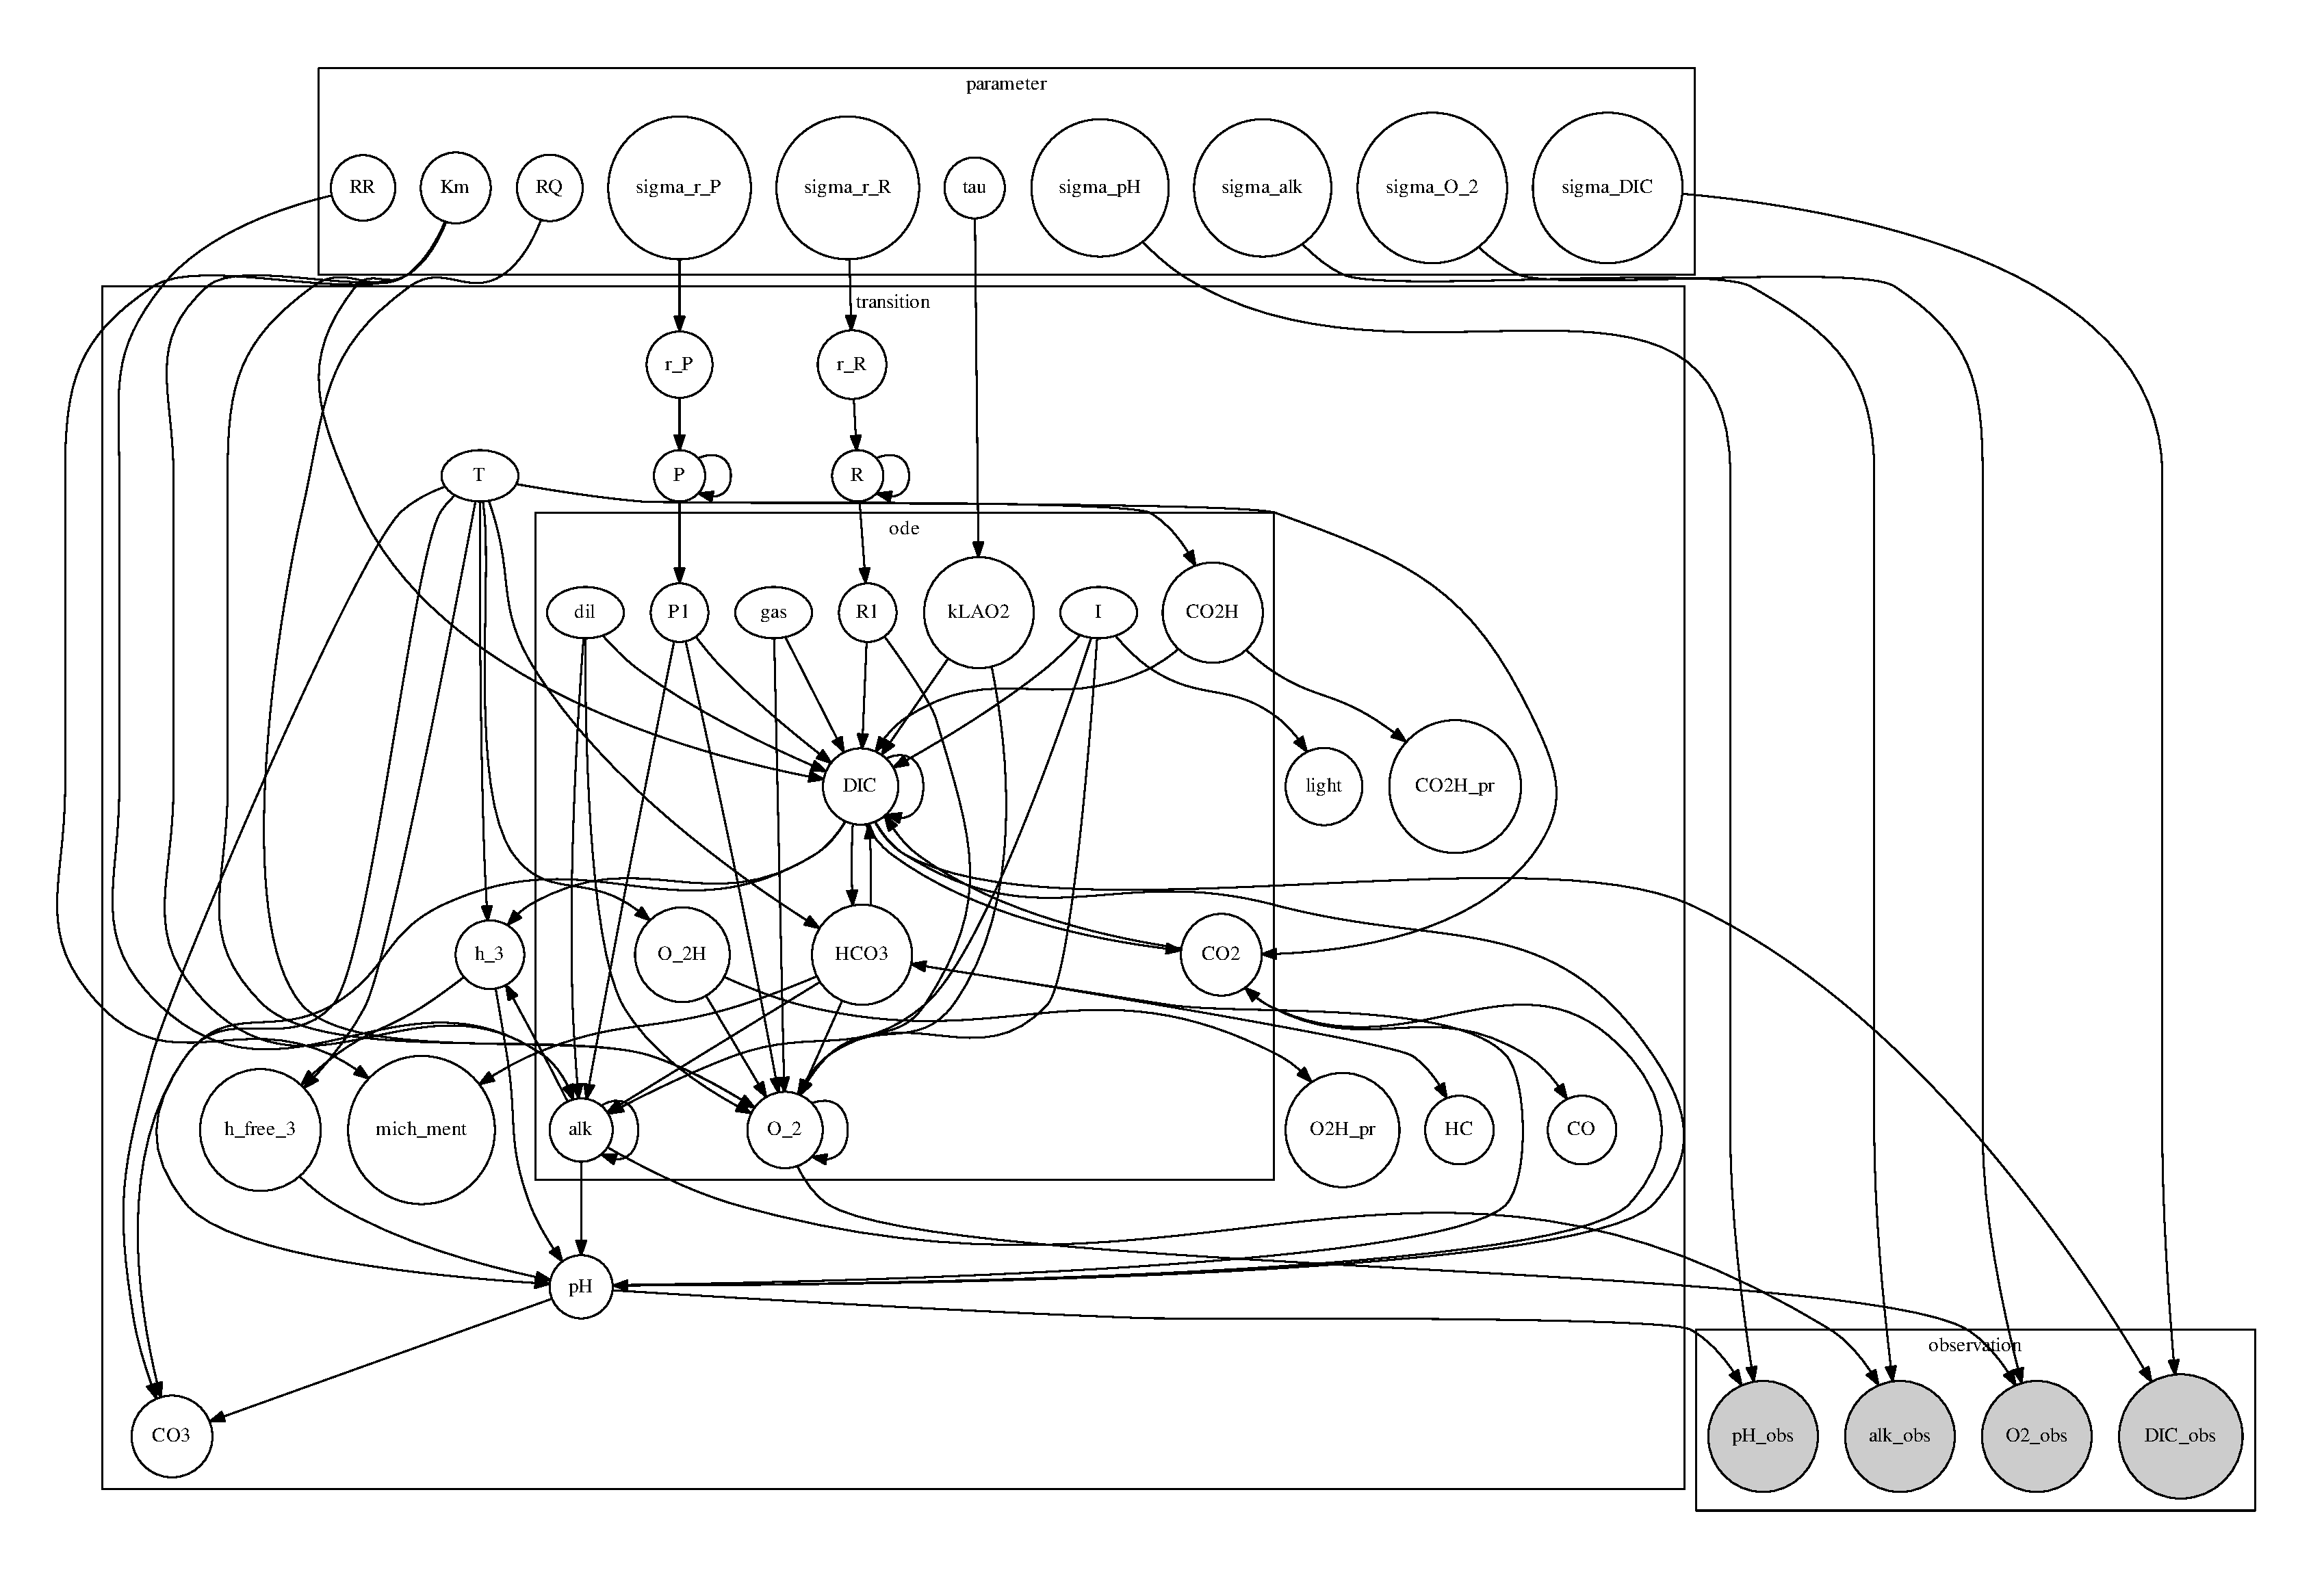
\includegraphics[width=0.9\textwidth]{images_microalgae/micro_template.pdf}}
	\caption[.]{Directed Acyclic Graph of the LiBbi model file micro\_iterative.bi}
	\label{fig:micro_DAG}
\end{sidewaysfigure}


\begin{figure}
	\centerline{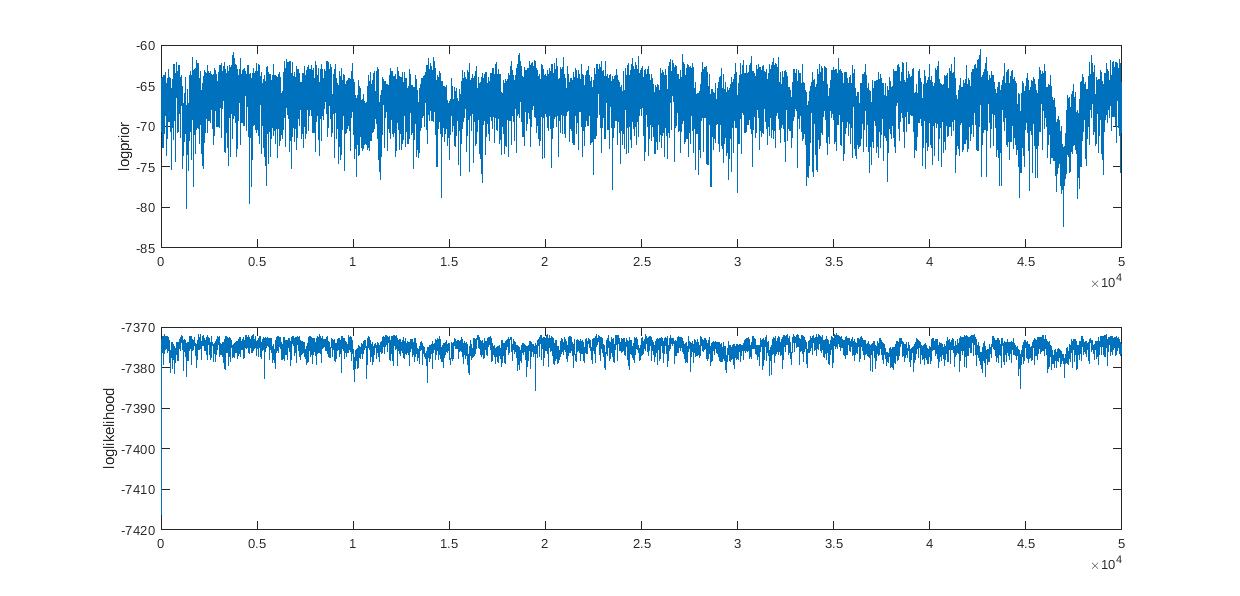
\includegraphics[width=1.3\textwidth]{images_microalgae/posterior_plots_with_fake_data/loglikelihood}}
	\caption[.]{Log-prior and log-likelihood for the simulated data experiment.}
	\label{fig:micro_sim_loglikelihood}
\end{figure}

\begin{figure}
	\centerline{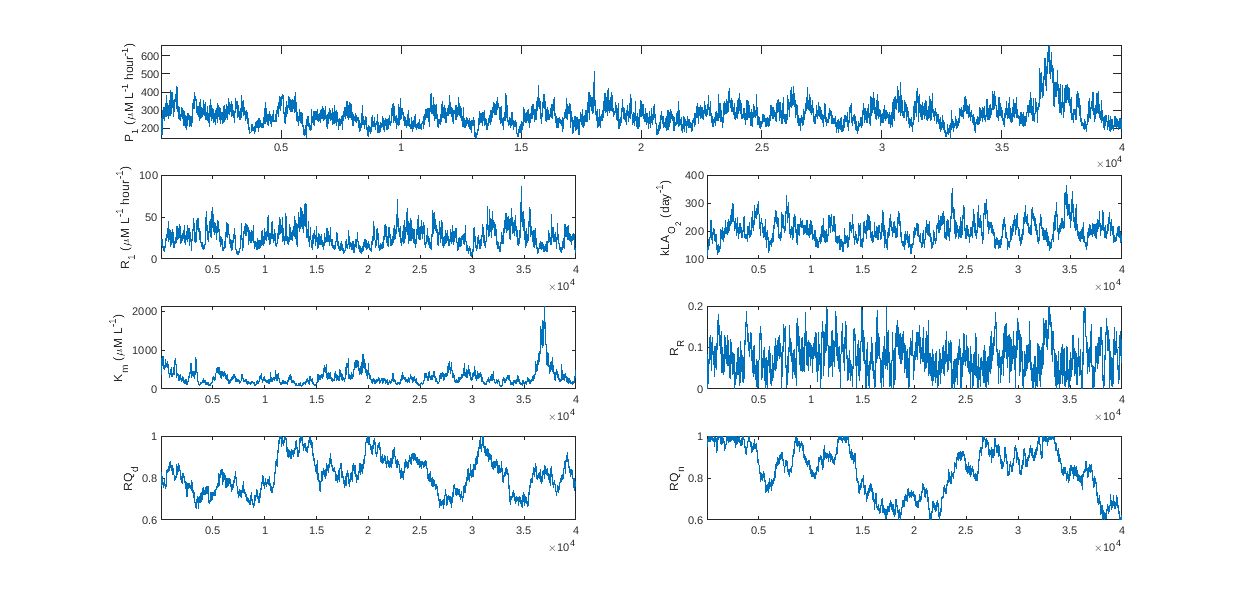
\includegraphics[width=1.3\textwidth]{images_microalgae/posterior_plots_with_fake_data/model_parameters_traces}}
	\caption[.]{Parameter posterior traces for the simulated data experiment.}
	\label{fig:micro_sim_model_parameters_traces}
\end{figure}


\FloatBarrier
\chapter{Posteriors with experimental data (photosynthesis, respiration and respiratory quotients are random walks, and an offset, and estimating obs error)}
% micro_iterative_chris_offset_sigma.bi

[BM: this is using the further thinned out observations too]

State posteriors are visualised by plotting the median and shading 95\% credible intervals, while parameter priors and posteriors are displayed by histograms.

\textbf{In this run:}\\
Photosynthesis ($P_1$) and respiration ($R_1$) are both modelled as random walks, by taking \begin{math}P\end{math} and \begin{math}R\end{math}, previously constant parameters, and replacing them by \begin{math}P_1(t)\end{math} and \begin{math}R_1(t)\end{math}. Here, we take \begin{math}P_1(t)\end{math} and \begin{math}R_1(t)\end{math} to be such that
\begin{displaymath}
P_1(t+\Delta t) = P(t) + r_P
\end{displaymath}
\begin{displaymath}
R_1(t+\Delta t) = R(t) + r_R
\end{displaymath}
where \begin{math}
r_P \sim N(0, \sigma_{r_P})
\end{math}, \begin{math}
r_R \sim N(0, \sigma_{r_R})
\end{math}, and \begin{math}
\Delta t
\end{math} is the length of discrete time-step. For the purpose of the Bayesian analysis here, \begin{math}\sigma_{r_P}\end{math} and \begin{math}\sigma_{r_R}\end{math} are treated as parameters to be inferred.  
The respiratory quotients $RQ_d$ and $RQ_n$ were also treated as random walks with $rP$ and $rR$ as wiener processes. 
$kLA_{O_2}$, $K_m$, $R_R$, $\sigma_{rP}$, $\sigma_{rR}$ are all treated as parameters constant through time but unknown. 
The data model assigned log normally distributed observation errors for each instrument;\\
$O_{2_{obs}}$ $\sim$ Log$\mathcal{N}$(log($O_2$), $\sigma_{O_2}$)\\
$pH_{obs}$ $\sim$ Log$\mathcal{N}$(log($pH$),  $\sigma_{pH}$)\\
$DIC_{obs}$ $\sim$ Log$\mathcal{N}$(log($DIC$), $\sigma_{DIC}$)\\
$TA_{obs}$ $\sim$ Log$\mathcal{N}$(log($TA$), $\sigma_{DIC}$)\\

\FloatBarrier
\begin{tabular}{c | c  |  c}
	\hline
	\bfseries{Parameter} & \bfseries{Prior} &  \bfseries{Proposal} \\ \hline
	$kLA_{O2}$  & Log$\mathcal{N}$(log(200.0), 0.3)  & Log$\mathcal{N}$(log($kLA_{O2}$), 0.03) \\
	$K_m$ 		&  Log$\mathcal{N}$(log(200.0), 0.6) & Log$\mathcal{N}$(log($K_m$), 0.06) \\
	$R_R$  		& Uniform(0, 0.2) &  Trun$\mathcal{N}$($R_R$, 0.005, lower = 0, upper = 0.2) \\
	%	$RQ_d$  	& Uniform(0.6, 1) &  Trun$\mathcal{N}$($RQ_d$, 0.005, lower = 0.6, upper = 1.0)\\
	%	$RQ_n$  	& Uniform(0.6, 1) &  Trun$\mathcal{N}$($RQ_n$, 0.005, lower = 0.6, upper = 1.0)\\
	$\sigma_{r_P}$ & $\mathcal{N}$(0.02, 0.002)   & $\mathcal{N}$($\sigma_{r_P}$, 0.0002)   \\
	$\sigma_{r_R}$ & $\mathcal{N}$(0.01, 0.001)   & $\mathcal{N}$($\sigma_{r_R}$, 0.0001)   \\
	$offset_{O_2}$ & $\mathcal{N}$(0, 5.0)     & $\mathcal{N}$($offset_{O_2}$, 0.5)   \\
	$\sigma_{O_2}$ 	& 0.1 	& * \\
	$\sigma_{pH}$ 	& 0.1 	& * \\
	$\sigma_{DIC}$ 	& 0.2 	& * \\	
\end{tabular}
\captionof{table}{Table of Parameters, their priors and proposal distributions. * indicates the parameter was held fixed.}

\FloatBarrier



\begin{figure}
	\centerline{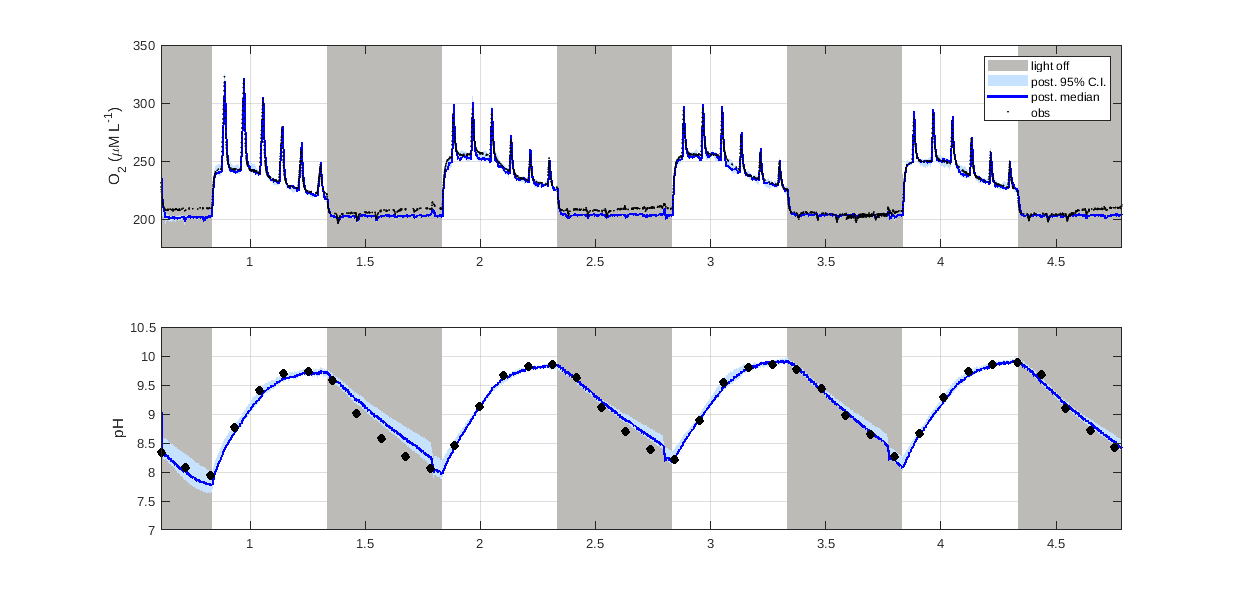
\includegraphics[width=1.2\textwidth]{images_microalgae/plots_chris_offset_sigma/O2_pH}}
	\caption[.]{Posterior medians (solid blue line), 95\% credible intervals (shaded blue), and simulated observations (black) for $O_2$ and $pH$ across 4 days.}
	\label{fig:micro_exp_offset_sigma_O2_pH}
\end{figure}

\begin{figure}
	\centerline{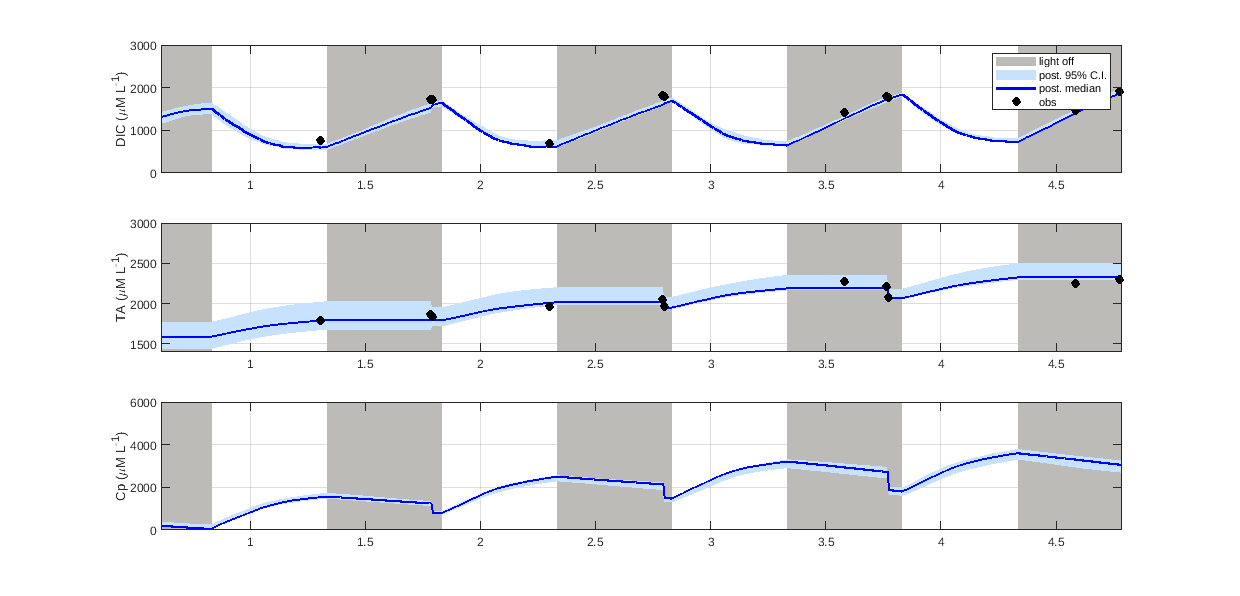
\includegraphics[width=1.2\textwidth]{images_microalgae/plots_chris_offset_sigma/DIC_TA_Cp}}
	\caption[.]{Posterior medians (solid blue line), 95\% credible intervals (shaded blue), and simulated observations (black) for $DIC$, $TA$ and $C_p$ across 4 days.}
	\label{fig:micro_exp_offset_sigma_DIC_TA_Cp}
\end{figure}

\begin{figure}
	\centerline{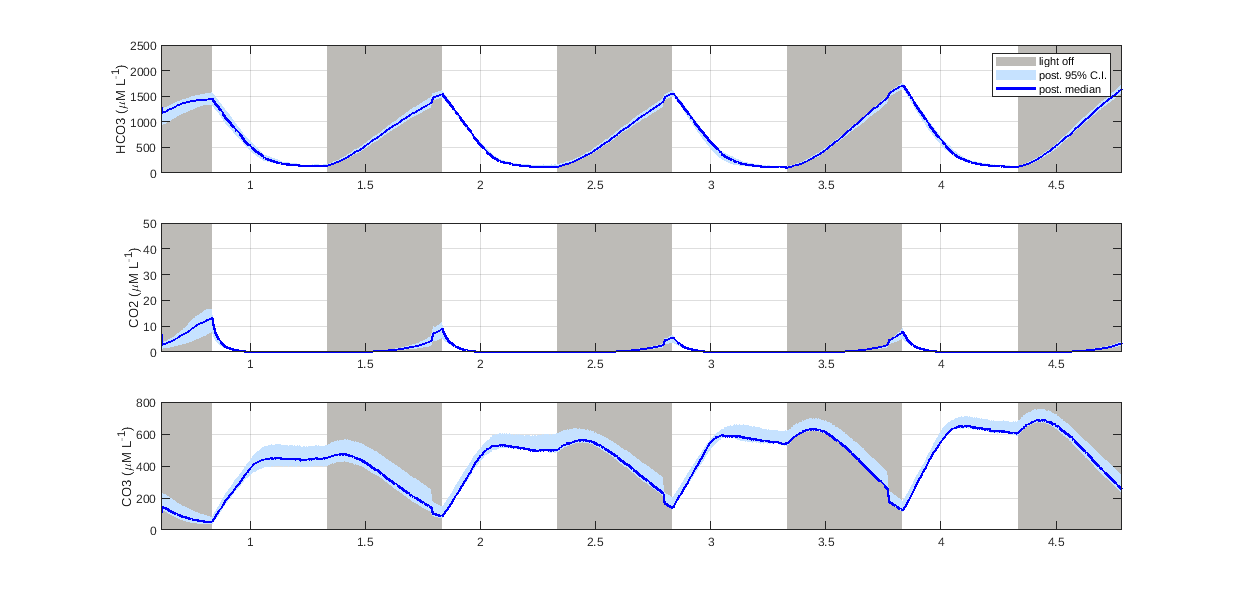
\includegraphics[width=1.2\textwidth]{images_microalgae/plots_chris_offset_sigma/carbon}}
	\caption[.]{Posterior medians (solid blue line) and 95\% credible intervals (shaded blue) for $HCO_3$, $CO_2$ and $CO_3$ across 4 days.}
	\label{fig:micro_exp_offset_sigma_carbon}
\end{figure}

\begin{figure}
	\centerline{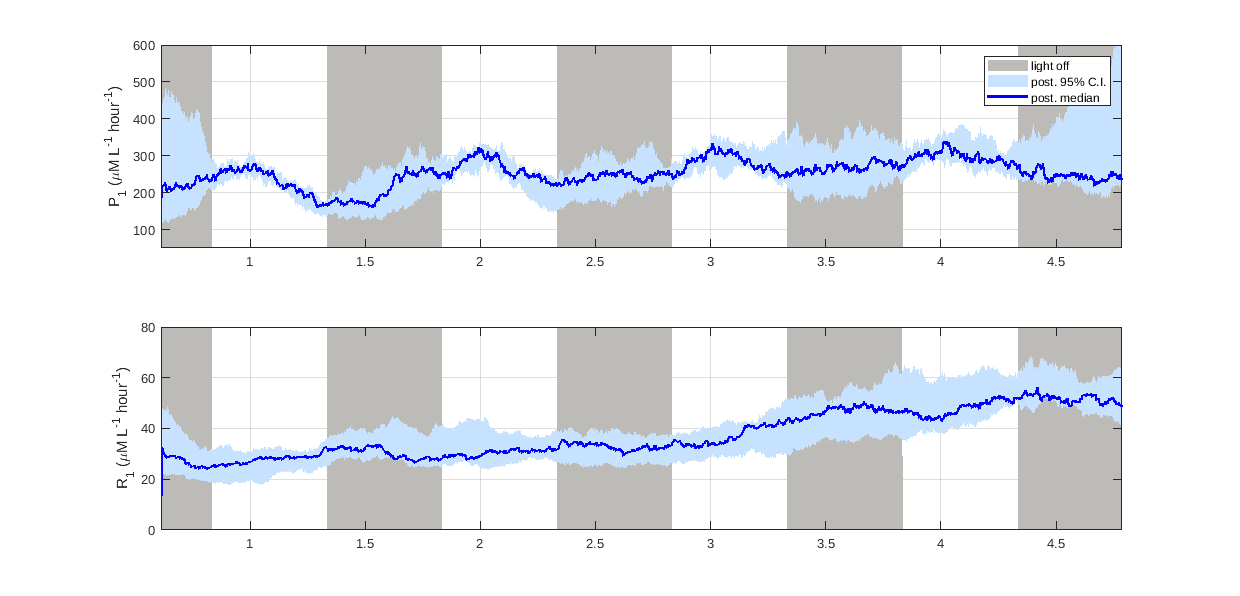
\includegraphics[width=1.2\textwidth]{images_microalgae/plots_chris_offset_sigma/P_and_R}}
	\caption[.]{Posterior medians (solid blue line) and 95\% credible intervals (shaded blue) for photosynthesis $P_1$ and respiration $R_1$.}
	\label{fig:micro_exp_offset_sigma_P_R}
\end{figure}

\begin{figure}
	\centerline{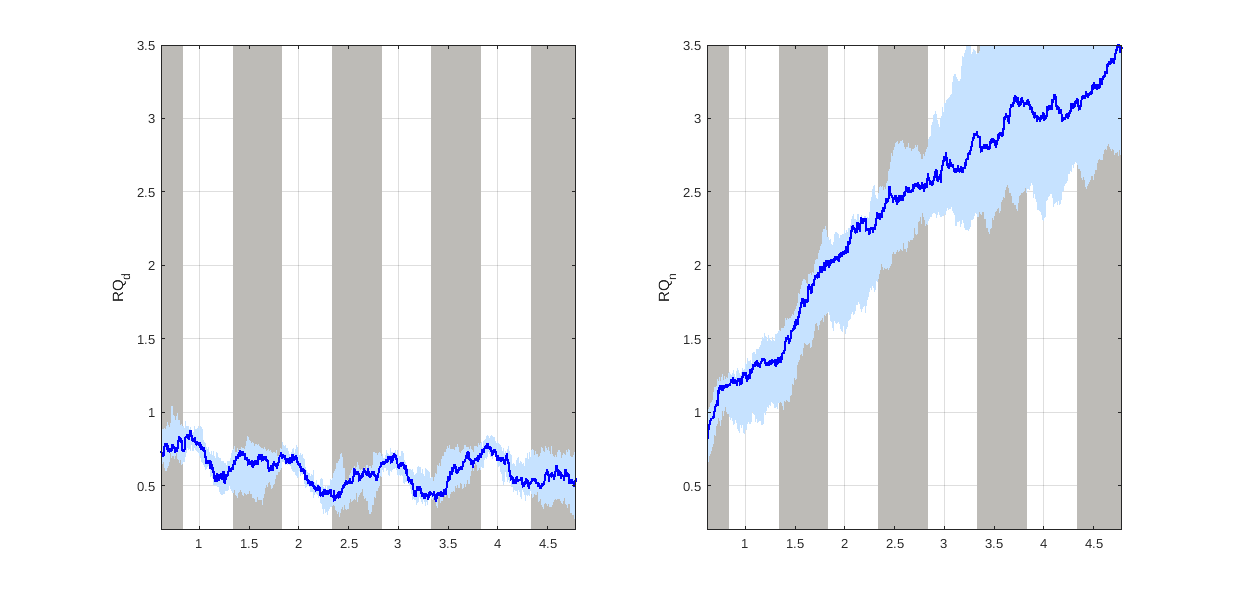
\includegraphics[width=1.2\textwidth]{images_microalgae/plots_chris_offset_sigma/RQ_d_RQ_n}}
	\caption[.]{Posterior medians (solid blue line) and 95\% credible intervals (shaded blue) for $RQ_d$ and $RQ_n$.}
	\label{fig:micro_exp_offset_sigma_RQ_d_RQ_n}
\end{figure}



\begin{figure}
	\centerline{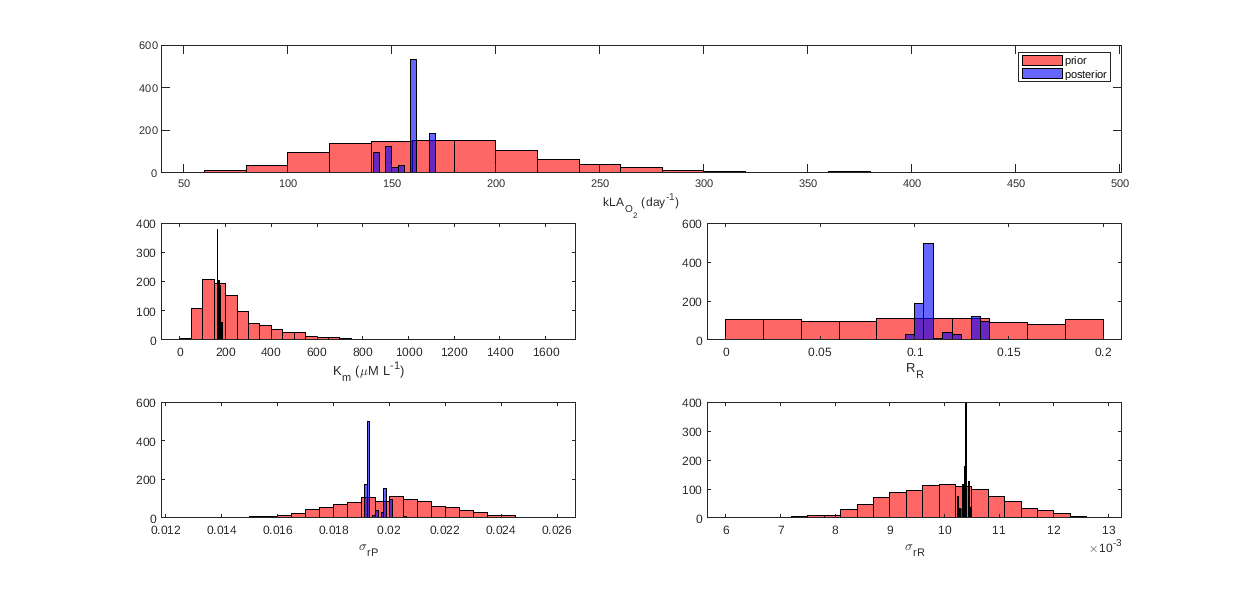
\includegraphics[width=1.3\textwidth]{images_microalgae/plots_chris_offset_sigma/modelparameters1}}
	\caption[.]{Priors (pink) and posteriors (purple) for model parameters.}
	\label{fig:micro_exp_offset_sigma_parameters_model}
\end{figure}

\begin{figure}
	\centerline{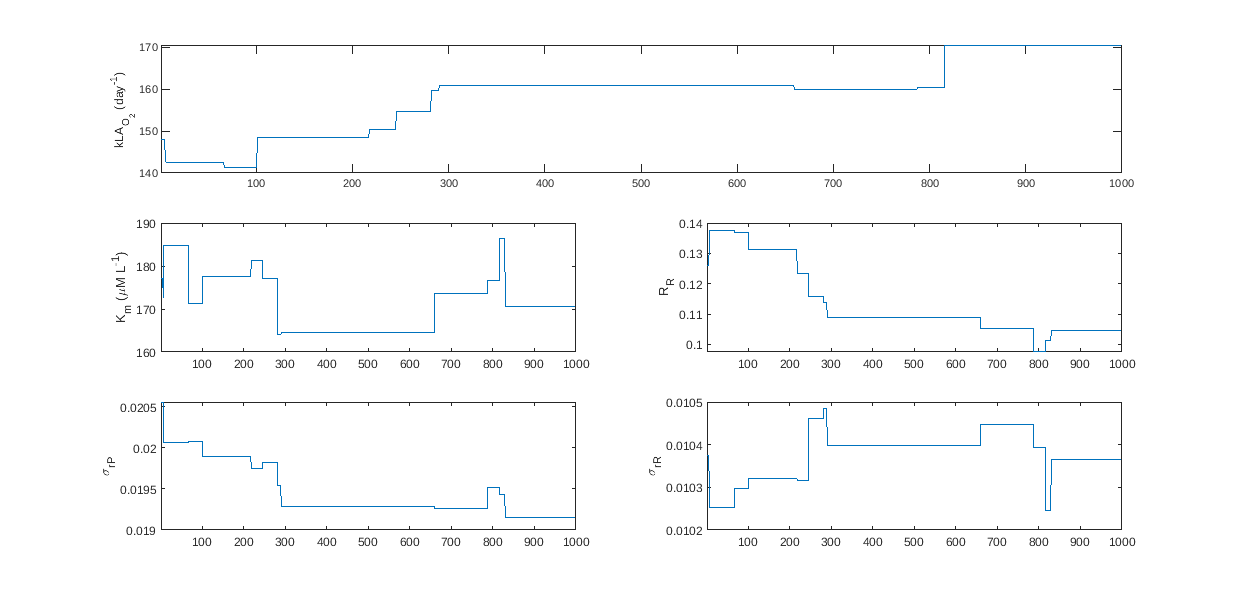
\includegraphics[width=1.3\textwidth]{images_microalgae/plots_chris_offset_sigma/modelparameters1_traces}}
	\caption[.]{Traces for model parameters.}
	\label{fig:micro_exp_offset_sigma_parameters_model2}
\end{figure}

\begin{figure}
	\centerline{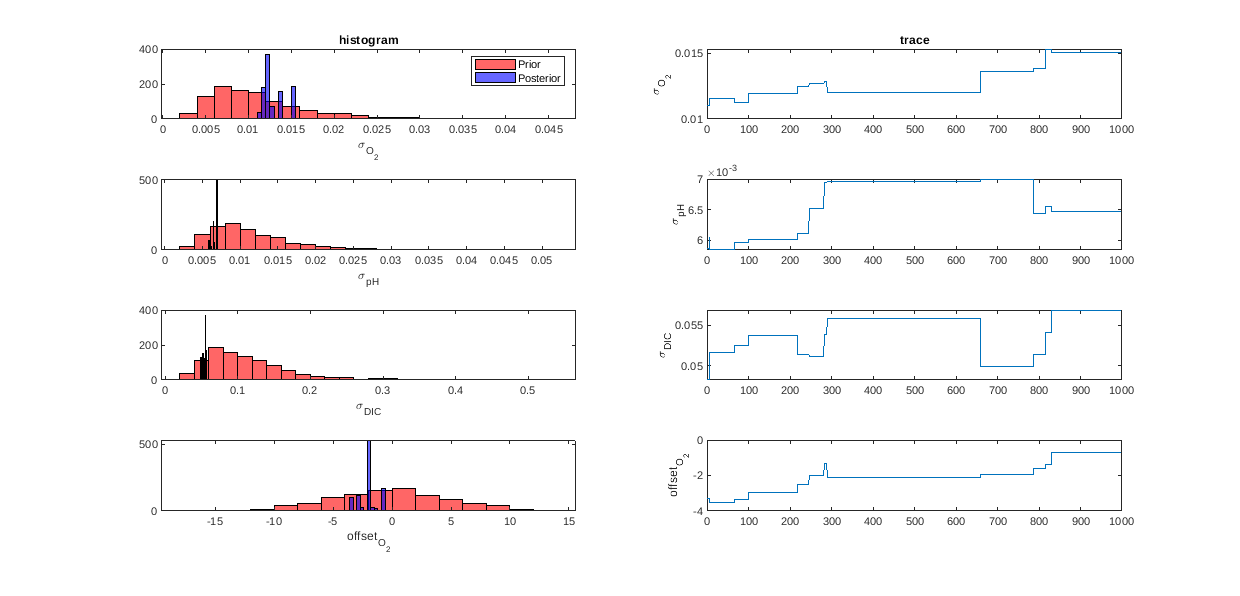
\includegraphics[width=1.3\textwidth]{images_microalgae/plots_chris_offset_sigma/sigmas}}
	\caption[.]{Priors (pink), posteriors (purple), and traces for observation error and offset model parameters.}
	\label{fig:micro_exp_offset_sigma_sigmas}
\end{figure}



\begin{longtable}{|c|c|c|} 
	\hline
	\bfseries{Parameter}  & \bfseries{Quantiles (25\%, 75\%)}  & \bfseries{Quantiles (5\%, 95\%)} \\ \hline
	$kLA_{O_2}^{air}$ 	& ()  		& ()   		\\
	$K_m$ 				& () 		& () 	 	\\ 
	$R_R$ 				& () 		& () 		 \\
	$\sigma_{r_P}$ 		& () 		& () 		 \\ 
	$\sigma_{r_R}$ 		& () 		& ()		 \\ 
	$offset_{O_2}$ 		& () 		& ()		 \\ 
	$\sigma_{O_2}$ 		& () 		& ()		 \\ 
	$\sigma_{pH}$ 		& () 		& ()		 \\ 
	$\sigma_{DIC}$ 		& () 		& ()		 \\ 	
	\hline
	\caption[.]{Posterior (25\%, 75\%), (5\%, 95\%) quantiles for parameters after assimilating observations.}	
	\label{table:micro_exp_offset_sigma_parameters_table}
\end{longtable}

\textbf{Results:}\\
The further thinned observations were used to test 1,000 samples with 2048 particles, returning an acceptance rate of 1.3\%.


\FloatBarrier
\chapter{Posterior results with experimental data where respiratory quotients are changing through time and bounded to biologically feasible values}
% micro_iterative.bi

\textbf{In this run:}\\
Photosynthesis ($P_1$) and respiration ($R_1$) were both modelled as random walks, by taking \begin{math}P\end{math} and \begin{math}R\end{math}, previously constant parameters, and replacing them by \begin{math}P_1(t)\end{math} and \begin{math}R_1(t)\end{math}. Here, we take \begin{math}P_1(t)\end{math} and \begin{math}R_1(t)\end{math} to be such that
\begin{displaymath}
P_1(t+\Delta t) = P(t) + r_P
\end{displaymath}
\begin{displaymath}
R_1(t+\Delta t) = R(t) + r_R
\end{displaymath}
where \begin{math}
r_P \sim N(0, \sigma_{r_P})
\end{math}, \begin{math}
r_R \sim N(0, \sigma_{r_R})
\end{math}, and \begin{math}
\Delta t
\end{math} is the length of discrete time-step. For the purpose of the Bayesian analysis here, \begin{math}\sigma_{r_P}\end{math} and \begin{math}\sigma_{r_R}\end{math} are treated as parameters to be inferred.  
The respiratory quotients ($RQ_d$ and $RQ_n$) are treated as normally distributed noisy states, truncated between 0.6 and 1, where the mean and standard deviation are unknown parameters to be estimated. \\
$
RQ_d \sim truncated\mathcal{N}(\mu_{RQ_d}, \sigma_{RQ_d}, lower = 0.6, upper = 1.0) \\
RQ_n \sim truncated\mathcal{N}(\mu_{RQ_n}, \sigma_{RQ_n}, lower = 0.6, upper = 1.0) \\ $

$kLA_{O_2}$, $K_m$, $R_R$, $\sigma_{rP}$, $\sigma_{rR}$, $\mu_{RQ_d}$, $\sigma_{RQ_d}$, $\mu_{RQ_n}$, $\sigma_{RQ_n}$ are all treated as parameters constant through time but unknown. 


\begin{longtable}{|c | c  |  c|}
	\hline
	\bfseries{Parameter} & \bfseries{Prior} &  \bfseries{Proposal} \\ \hline
	$kLA_{O2}$  & Log$\mathcal{N}$(log(200.0), 0.3)  & Log$\mathcal{N}$(log($kLA_{O2}$), 0.03) \\
	$K_m$ 		&  Log$\mathcal{N}$(log(200.0), 0.6) & Log$\mathcal{N}$(log($K_m$), 0.06) \\
	$R_R$  		& Uniform(0, 0.2) &  Trun$\mathcal{N}$($R_R$, 0.01, lower = 0, upper = 0.2) \\
	$\mu_{RQ_d}$  	& Uniform(0.6, 1) &  $\mathcal{N}$($\mu_{RQ_d}$, 0.01)\\
	$\mu_{RQ_n}$  	& Uniform(0.6, 1) &  $\mathcal{N}$($\mu_{RQ_n}$, 0.01)\\
	$\sigma_{RQ_d}$ & Uniform(0, 0.5) &  $\mathcal{N}$($\sigma_{RQ_d}$, 0.01)\\
	$\sigma_{RQ_n}$ & Uniform(0, 0.5) &  $\mathcal{N}$($\sigma_{RQ_n}$, 0.01)\\
	$\sigma_{r_P}$ & $\mathcal{N}$(0.01, 0.001)   & $\mathcal{N}$($\sigma_{r_P}$, 0.0001)   \\
	$\sigma_{r_R}$ & $\mathcal{N}$(0.01, 0.001)   & $\mathcal{N}$($\sigma_{r_R}$, 0.0001)   \\
	$\sigma_{O_2}$ 	& 0.4	& *  \\
	$\sigma_{pH}$ 	& 0.4 	& * \\
	$\sigma_{DIC}$ 	& 0.4	& * \\
	\hline	
	\caption[.]{Table of Parameters, their priors and proposal distributions (* indicates the parameter was held fixed).}
\end{longtable}




\begin{figure}
	\centerline{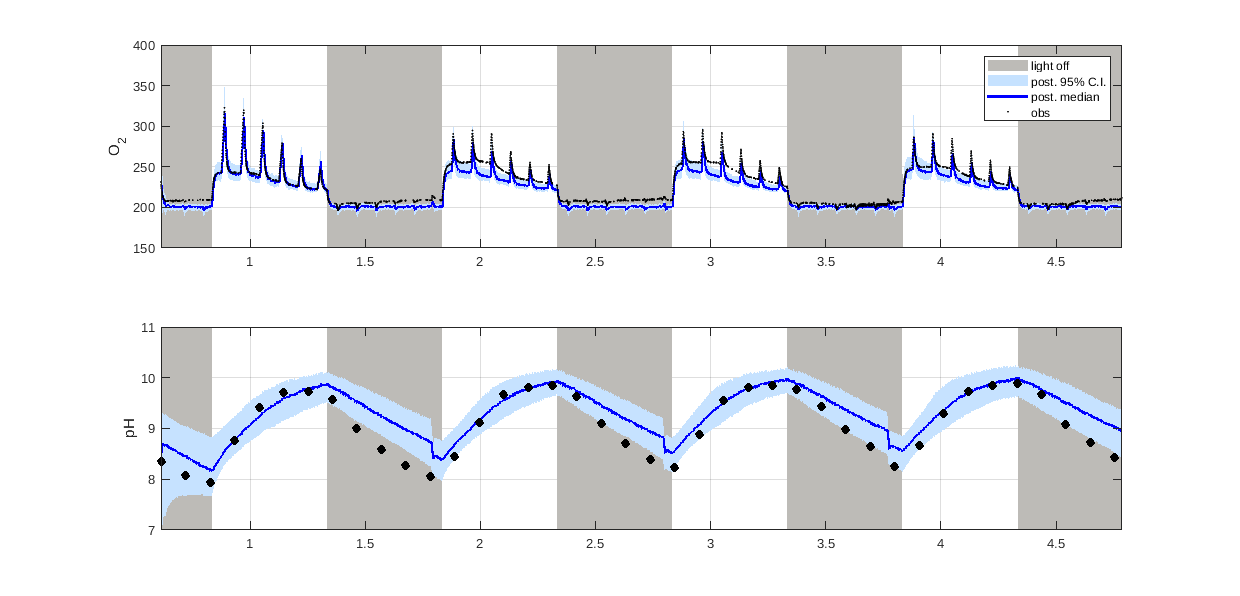
\includegraphics[width=1.2\textwidth]{images_microalgae/plots_iterative/O2_pH}}
	\caption[.]{Posterior medians (solid blue line), 95\% credible intervals (shaded blue), and simulated observations (black) for $O_2$ and $pH$ across 4 days.}
	\label{fig:micro_exp_iterative_O2_pH}
\end{figure}

\begin{figure}
	\centerline{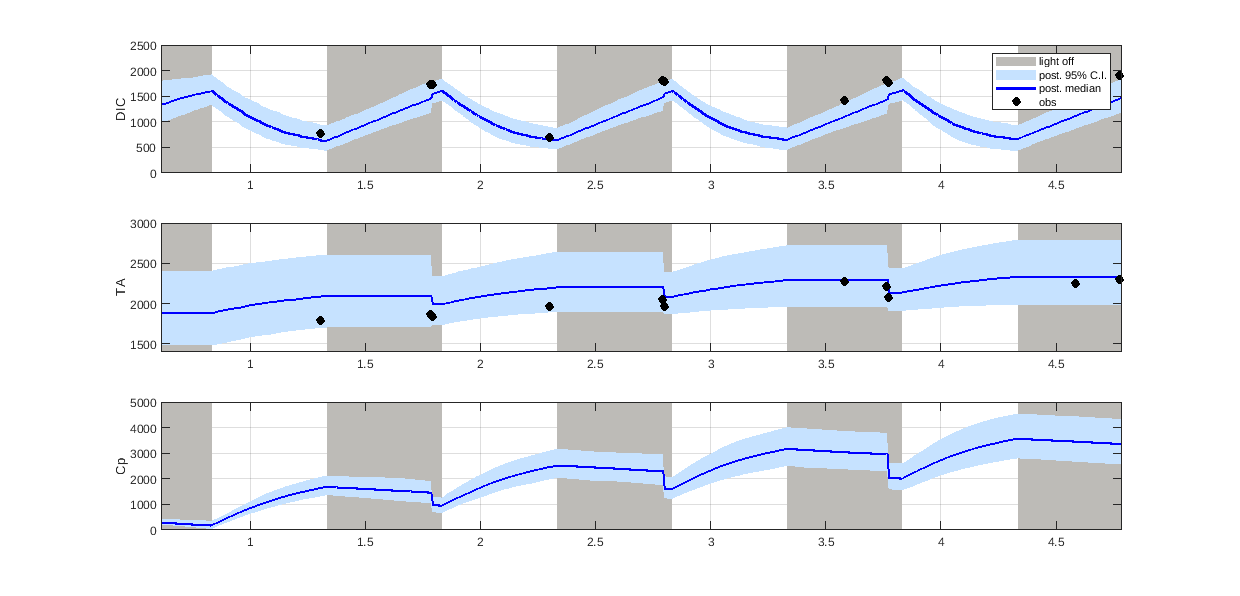
\includegraphics[width=1.2\textwidth]{images_microalgae/plots_iterative/DIC_TA_Cp}}
	\caption[.]{Posterior medians (solid blue line), 95\% credible intervals (shaded blue), and simulated observations (black) for $DIC$, $TA$ and $C_p$ across 4 days.}
	\label{fig:micro_exp_iterative_DIC_TA_Cp}
\end{figure}

\begin{figure}
	\centerline{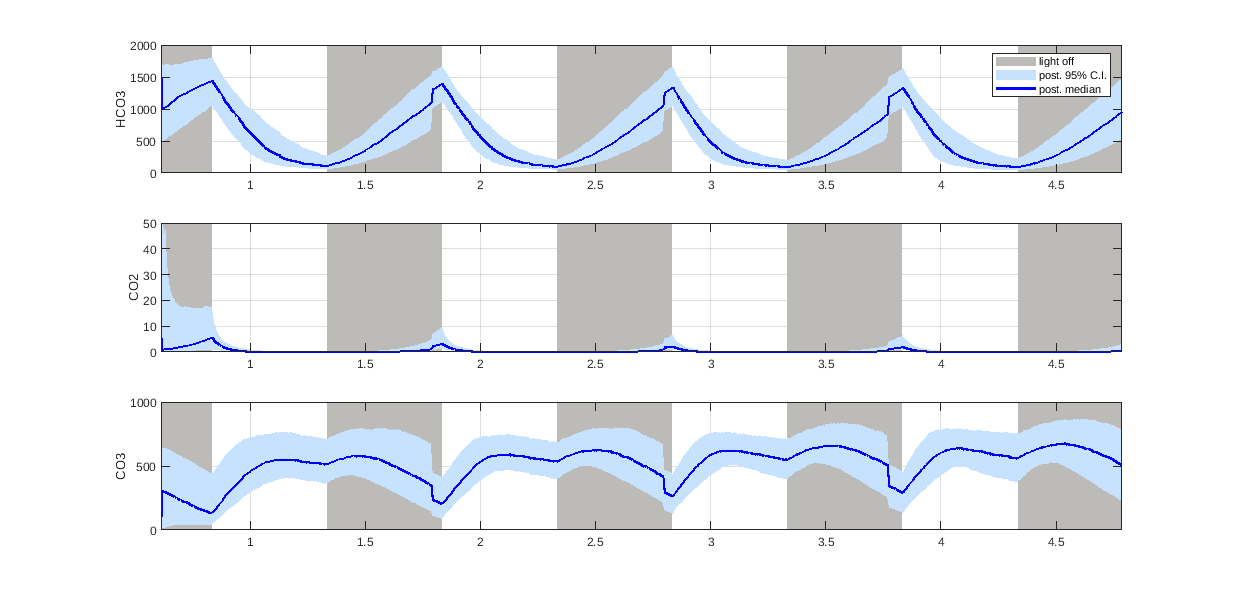
\includegraphics[width=1.2\textwidth]{images_microalgae/plots_iterative/carbon}}
	\caption[.]{Posterior medians (solid blue line) and 95\% credible intervals (shaded blue) for $HCO_3$, $CO_2$ and $CO_3$ across 4 days.}
	\label{fig:micro_exp_iterative_carbon}
\end{figure}

\begin{figure}
	\centerline{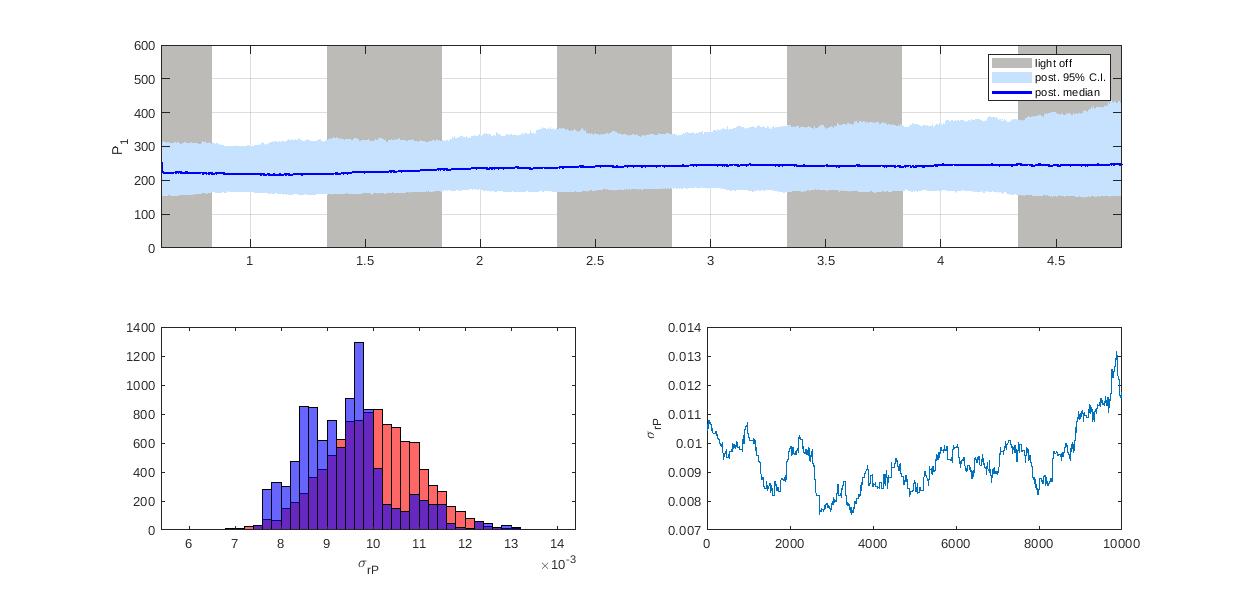
\includegraphics[width=1.2\textwidth]{images_microalgae/plots_iterative/P}}
	\caption[.]{Posterior medians (solid blue line) and 95\% credible intervals (shaded blue) for photosynthesis $P_1$.}
	\label{fig:micro_exp_iterative_P}
\end{figure}

\begin{figure}
	\centerline{\includegraphics[width=1.2\textwidth]{images_microalgae/plots_iterative/R}}
	\caption[.]{Posterior medians (solid blue line) and 95\% credible intervals (shaded blue) for respiration $R_1$.}
	\label{fig:micro_exp_iterative_R}
\end{figure}

\begin{figure}
	\centerline{\includegraphics[width=1.2\textwidth]{images_microalgae/plots_iterative/RQ_d}}
	\caption[.]{Posterior medians (solid blue line) and 95\% credible intervals (shaded blue) for $RQ_d$.}
	\label{fig:micro_exp_iterative_RQ_d}
\end{figure}

\begin{figure}
	\centerline{\includegraphics[width=1.2\textwidth]{images_microalgae/plots_iterative/RQ_n}}
	\caption[.]{Posterior medians (solid blue line) and 95\% credible intervals (shaded blue) for $RQ_n$.}
	\label{fig:micro_exp_iterative_RQ_n}
\end{figure}

\begin{figure}
	\centerline{\includegraphics[width=1.3\textwidth]{images_microalgae/plots_iterative/model_parameters}}
	\caption[.]{Priors (pink) and posteriors (purple) for model parameters.}
	\label{fig:micro_exp_iterative_parameters_model}
\end{figure}


\textbf{Results:}\\
10,000 samples run (no burn-in was discarded) with 1024 particles.
Updated version: 20,000 (10,000 discarded as burn-in) samples with 2048 particles.



\bibliography{seagrassbib}{}
\bibliographystyle{plain}

%\ifx\printbibliography\undefined
%\bibliographystyle{plain}
%\bibliography{bibexport}
%\else\printbibliography\fi



\end{document}

